\documentclass[11pt, a4paper]{book}
\usepackage[utf8]{inputenc}
\usepackage{multirow}
\usepackage{graphicx}
\graphicspath{ {../images} }

\usepackage[T1]{fontenc}


\usepackage[spanish, es-lcroman]{babel}
\usepackage{amsmath}
\usepackage{amsthm}
\usepackage{amsfonts}
\usepackage{amssymb}
\usepackage{titlesec}
\usepackage{enumerate}
\usepackage{enumitem}
\usepackage{graphicx}
\usepackage{mathtools}
\usepackage{array}
\usepackage{float}
\usepackage{pgfplots}
\usepackage{parskip}
\usetikzlibrary{fit,backgrounds}
\usepackage[]{hyperref}

\usepackage{changepage}
\usepackage{tikz}
\usepackage{nameref}

\usepackage[a4paper]{geometry}
\geometry{top=2.5cm, bottom=2.5cm, left=2.75cm, right=2.75cm}
\pagenumbering{arabic}

\usepackage{fancyhdr}
\pagestyle{fancy} 
\fancypagestyle{plain}{\fancyhf{}\fancyhead[L]{\quad\leftmark}\fancyhead[R]{\thepage}} 

\fancyhf{} % Limpia los encabezados y pies de página

% Configuración del encabezado
\fancyhead[L]{\quad\leftmark} % Muestra número de sección
\fancyhead[R]{\thepage}         % Número de página a la derecha

\usepackage{color}
\definecolor{editorGray}{rgb}{0.95, 0.95, 0.95}
\definecolor{editorOcher}{rgb}{1, 0.5, 0} % #FF7F00 -> rgb(239, 169, 0)
\definecolor{editorGreen}{rgb}{0, 0.5, 0} % #007C00 -> rgb(0, 124, 0)
\usepackage{upquote}
\usepackage{listings}
\lstdefinelanguage{JavaScript}{
	morekeywords={typeof, new, true, false, catch, function, return, null, catch, switch, var, if, in, while, do, else, case, break, let, const},
	morecomment=[s]{/*}{*/},
	morecomment=[l]//,
	morestring=[b]",
	morestring=[b]'
}

\lstdefinelanguage{HTML5}{
	language=html,
	sensitive=true, 
	alsoletter={<>=-},
	keywords={
		% HTML tags
		<html>, <head>, <title>, </title>, <meta, />, </head>, <body>,
		<canvas, \/canvas>, <script>, </script>, </body>, </html>, <!, html>, <style>, </style>, ><,
		% CSS
		@media
	},  
	ndkeywords={
		% General
		=,
		% HTML attributes
		charset=, id=, width=, height=,
		% CSS properties
		width:, max-width:, float:, display, border:, grid-template-areas:, grid-template-columns:, grid-template-rows:
	},  
	morecomment=[s]{<!--}{-->},
	tag=[s]
}

\lstset{%
	% Basic design
	backgroundcolor=\color{editorGray},
	basicstyle={\footnotesize\ttfamily},   
	frame=l,
	% Line numbers
	xleftmargin={0.75cm},
	numbers=left,
	stepnumber=1,
	firstnumber=1,
	numberfirstline=true,
	% Code design   
	keywordstyle=\color{editorOcher}\bfseries,
	commentstyle=\color{darkgray}\ttfamily,
	ndkeywordstyle=\color{blue}\bfseries,
	stringstyle=\color{editorGreen}, 
	% Code
	language=HTML5,
	alsolanguage=JavaScript,
	alsodigit={.:;},
	tabsize=3,
	showtabs=false,
	showspaces=false,
	showstringspaces=false,
	extendedchars=true,
	breaklines=true,        
}




\title{Título y portada chula}

\begin{document}
	\maketitle
	
	\tableofcontents
	\newpage
	\thispagestyle{empty}
	
	\chapter{Documentación inicial}
	
	\section{Introducción}
	\textbf{El Problema del Viajante} es una agencia de viajes ficticia en la que se ofrecerán todo tipo de servicios relacionados con la planificación y la gestión de viajes, incluyendo transporte, alojamiento, lugares de interés para visitar, ocio, restauración, etc.
	
	\textcolor{red}{------------ Hay que mejorar la intro, mínimo una carilla ---------}
	\textcolor{red}{Poner en algún lado que nosotros no hacemos las reservas como tal, solo lo ponemos bonito y redirigimos a otros lugares donde sí se puede reservar}
	
	El proyecto puede encontrarse en \href{https://github.com/PedroVidalVillalba/DAW_P1}{https://github.com/PedroVidalVillalba/DAW\_P1}, donde se encuentra también la última versión estable de este mismo documento y de la página web.
	
	
	Se han utilizado como inspiración diferentes páginas web de reserva de viajes, en especial \href{https://experiencetravelgroup.com}{Experience travel group}, aunque también se han consultado:
	\begin{itemize}
		\item \href{https://booking.com}{Booking}
		\item \href{https://tripadvisor.es}{Tripadvisor}
		\item \href{https://skyscanner.es}{Skyscanner}
		\item \href{https://calendar.google.com/calendar/u/0/r}{Google Calendar}
	\end{itemize}
	
	 En estas páginas se puede comprobar que es habitual ofrecer una experiencia lo más completa posible respecto a la organización desde el mismo lugar el transporte y alojamiento. Pero hemos echado en falta que ninguna tenga aspectos más relacionados con la planificación en el propio viaje, como lugares de interés o restaurantes, y que incluso se pueda acceder a la reserva desde la propia página, de forma que se cree un itinerario. Además, ya no sería necesario acceder a otro lugar para indicar en el calendario las fechas indicadas, sino que ya se mostrarían en la propia página, y este calendario podría sincronizarse con el de la cuenta de Google, u otros semejantes.
	
	
	
	\section{Inventario de contenido}
	Inicialmente se ha realizado una tormenta de ideas, en la que se ha reflexionado sobre el tema escogido, y su contenido, audiencia, elementos visuales atractivos para el usuario, etc. Los contenidos iniciales de la tormenta de ideas se pueden consultar en el \nameref{chap:anexo1}. Los elementos principales sobre los que se estructura la aplicación son:
	
	\begin{itemize}
		\item Reserva de hoteles, aviones y otros medios de transporte. En general, cómo ir desde el lugar donde vive el usuario hasta su destino.
		\item Lugares de interés para visitar, con fotos, su web, ubicación, etc. 
		\item Lugares de ocio, restauración, y otro tipo de tiendas conocidas en la zona.
		\item Calendario con planificación del viaje, desde el que acceder a la información sobre el medio de transporte elegido, alojamiento, etc. y que permita organizar los lugares de visita de cada día.
		\item Lista de lugares y tiendas favoritos, junto a un mapa integrado en donde aparezcan destacados.
		\item Experiencias exclusivas, con planificaciones de viajes realizadas previamente por expertos.
	\end{itemize} 
	
	Después de analizar los elementos obtenidos, filtrarlos y establecer relaciones entre sí, se ha llegado al siguiente inventario de contenido:

	\textcolor{red}{---------------Poner aquí el inventario de contenido. Hay que hacer un dibujín -------------------------}
	
	Otros elementos que también son relevantes para la justificación de la creación de la página web son:
	
	\begin{enumerate}
		\item \textbf{Audiencia}: un público genérico, ya que cada vez más personas viajan de forma relativamente habitual, y resulta de gran utilidad una página web desde la que poder gestionar todo el viaje.
		\item \textbf{Elementos visuales}: principalmente imágenes y vídeos de cada lugar, que deben llamar la atención del usuario sin ser excesivos, y también mapas. Se creará un logo generado con IA que sea característico de la empresa.
		\item \textbf{Financiación}: se podrían obtener beneficios a través de anuncios en la página. También se podría incluir un sistema de suscripción o mecenazgo con descuentos dentro de la página web, para clientes habituales.
	\end{enumerate}


	\section{Arquitectura de información}
	Una vez se dispone del inventario de contenido, se organizan estos elementos jerárquicamente en una arquitectura de la información, que dará una primera aproximación al número de páqinas que se necesitarán crear y al esquema de navegación que permite relacionarlas. 
	
	Se llega así, a alto nivel, a la siguiente estructura, en la que cada elemento principal tiene varias ramas:
	
	\begin{itemize}
		\item \textbf{Página principal}: presentación de la página que llame la atención, \textit{newsletter}, valoraciones, opiniones de expertos.
		\item \textbf{Descubre}: búsqueda de lugares visita, ocio, restauración etc., destinos de moda/recomendados, exploración, mapa de lugares favoritos.
		\item \textbf{Planifica}: calendario, consejos generales para viajes al extranjero, seguro de viajes, mecanismos de reserva con seguridad.
		\item \textbf{Reserva}: búsqueda de hoteles, búsqueda de aviones y otros medios de transporte, alquiler de coches, reserva de restaurantes, experiencias exclusivas.
		\item \textbf{About us}: quiénes somos, nuestra historia, qué nos diferencia, FAQ, redes sociales, nuestro sistema de puntuación, certificados de calidad, premios.
		\item \textbf{Otros}: términos de uso, política de cookies, política de privacidad.
	\end{itemize}

	\begin{figure} [H]
		\centering
		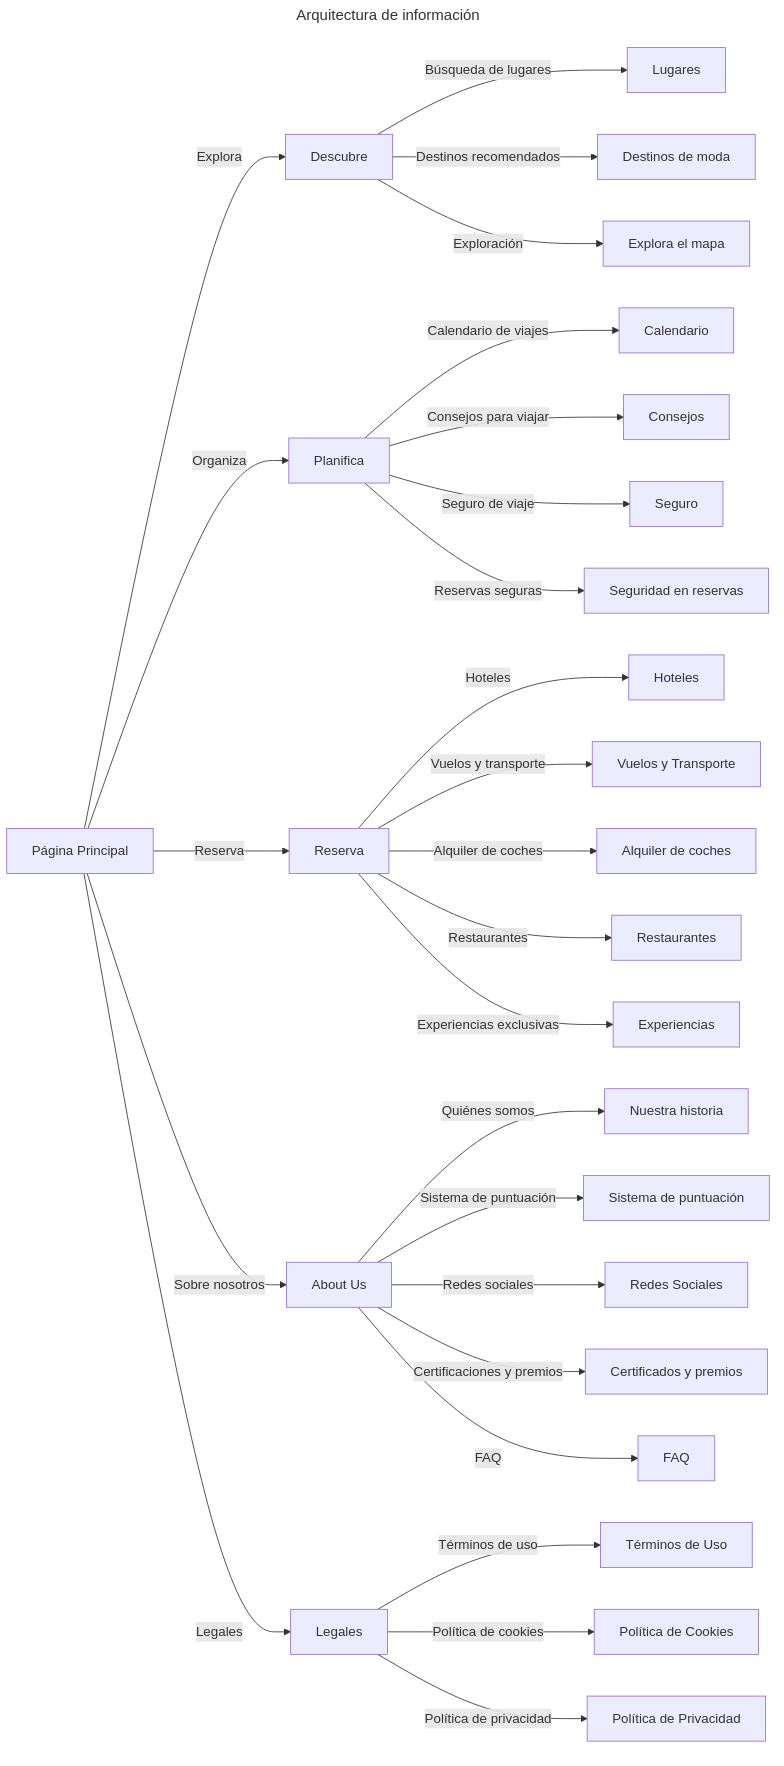
\includegraphics[height=0.85\textheight]{arquitectura_informacion.png}
		\caption{Arquitectura de información}
	\end{figure}
	
	
	
	\section{Mapa de navegación}
	El mapa de navegación plasma las relaciones jerárquicas recogidas por la arquitectura de la información y las organiza en páginas concretas que serán posteriormente implementables. Como se ve en la imagen, es similar a la arquitectura de información
	
	\begin{figure} [H]
		\centering
		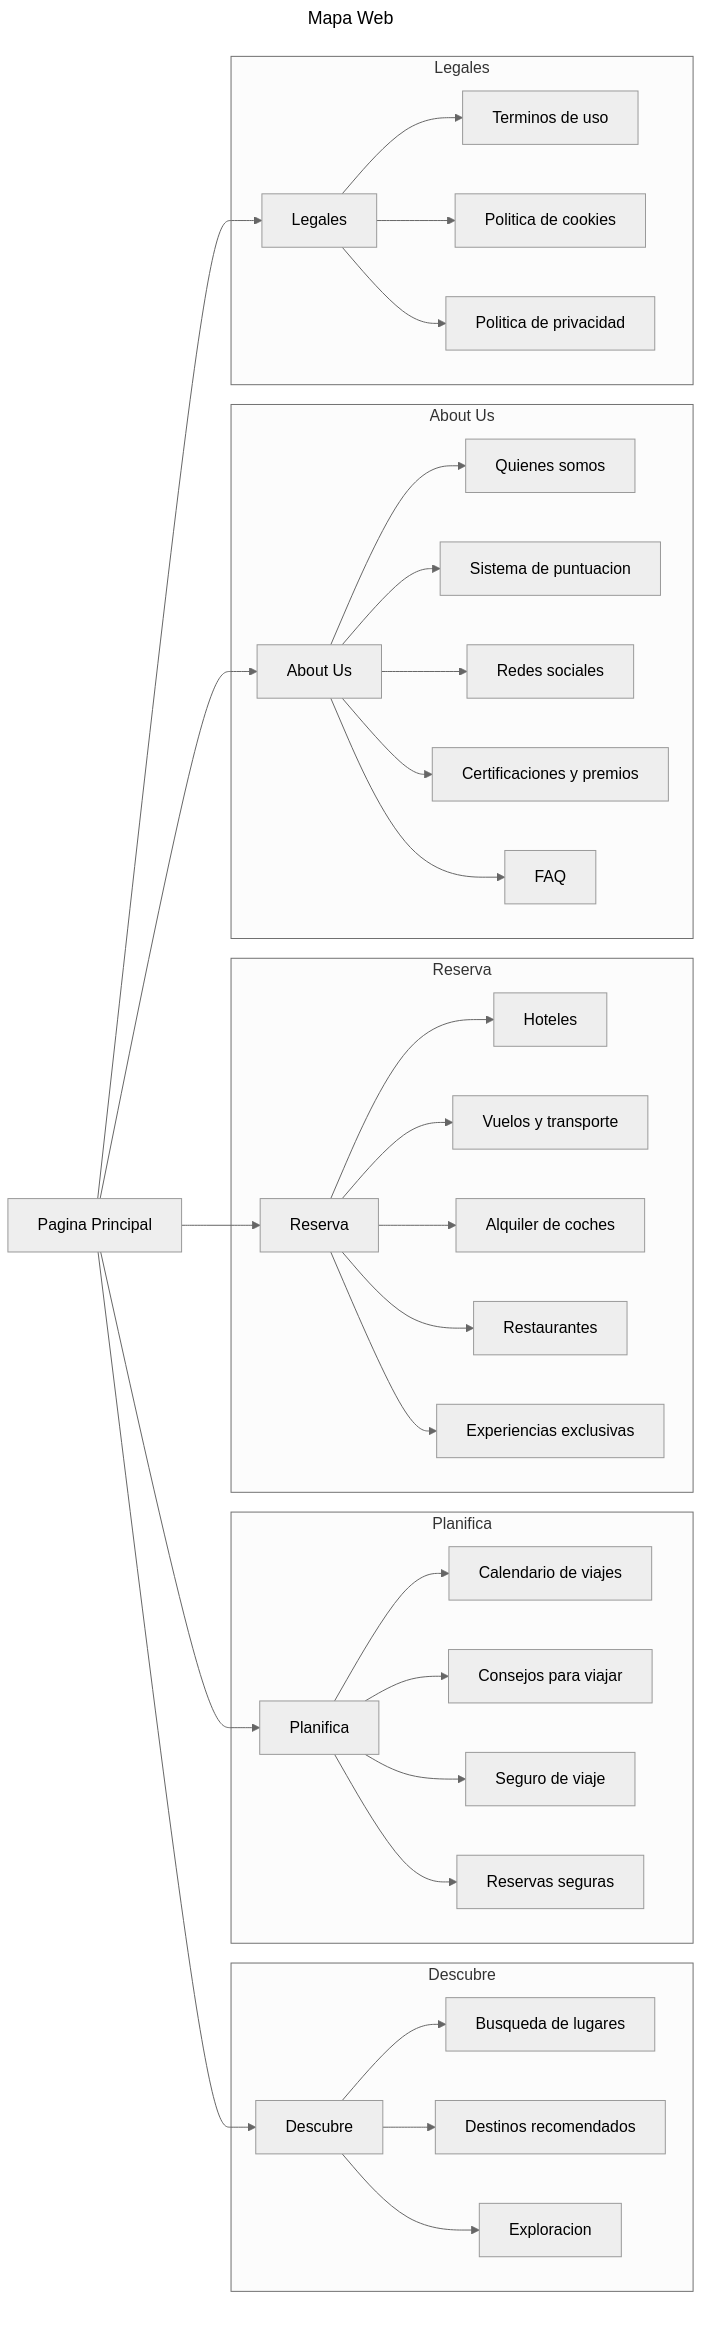
\includegraphics[height=0.8\textheight]{mapa_web.png}
		\caption{Mapa de navegación}
	\end{figure}
	
	
	
	\section{Interfaces}
	Con toda la información recogida, el siguiente paso es empezar a diseñar las interfaces, en las que se muestre un prototipo de la disposición, fuentes de texto, colores, imágenes y navegación en las diferentes páginas web. En este caso, se han realizado interfaces de las 5 páginas principales: la página principal, descubre, planifica, reserva y \textit{about us}. 
	
	Cada una incluye tres fases de desarrollo, una prototipo manual(\textit{sketch}) con las ideas básicas que conforman el sitio web, un esqueleto digital (\textit{wireframe}) centrado en la disposición de los elementos de acuerdo a proporciones adecuadas, y por último un diseño final (\textit{mockup}) de la interfaz, que muestra cómo debería ser la apariencia final de la página, incluyendo colores, fuentes de texto e imágenes adecuadas.
	
	\subsection{Prototipo manual}
	A continuación se muestran los bocetos de las interfaces realizadas a mano. Dado el carácter académico de este documento, se considera relevante incluirlas, a pesar de que en un entorno profesional su uso sería poco común. Se han realizado los prototipos para cinco ventanas, las cuales se comentan a continuación.
	
	\newpage % Mejor poner juntos imagen y descripción
	
	\begin{figure} [H]
		\centering
		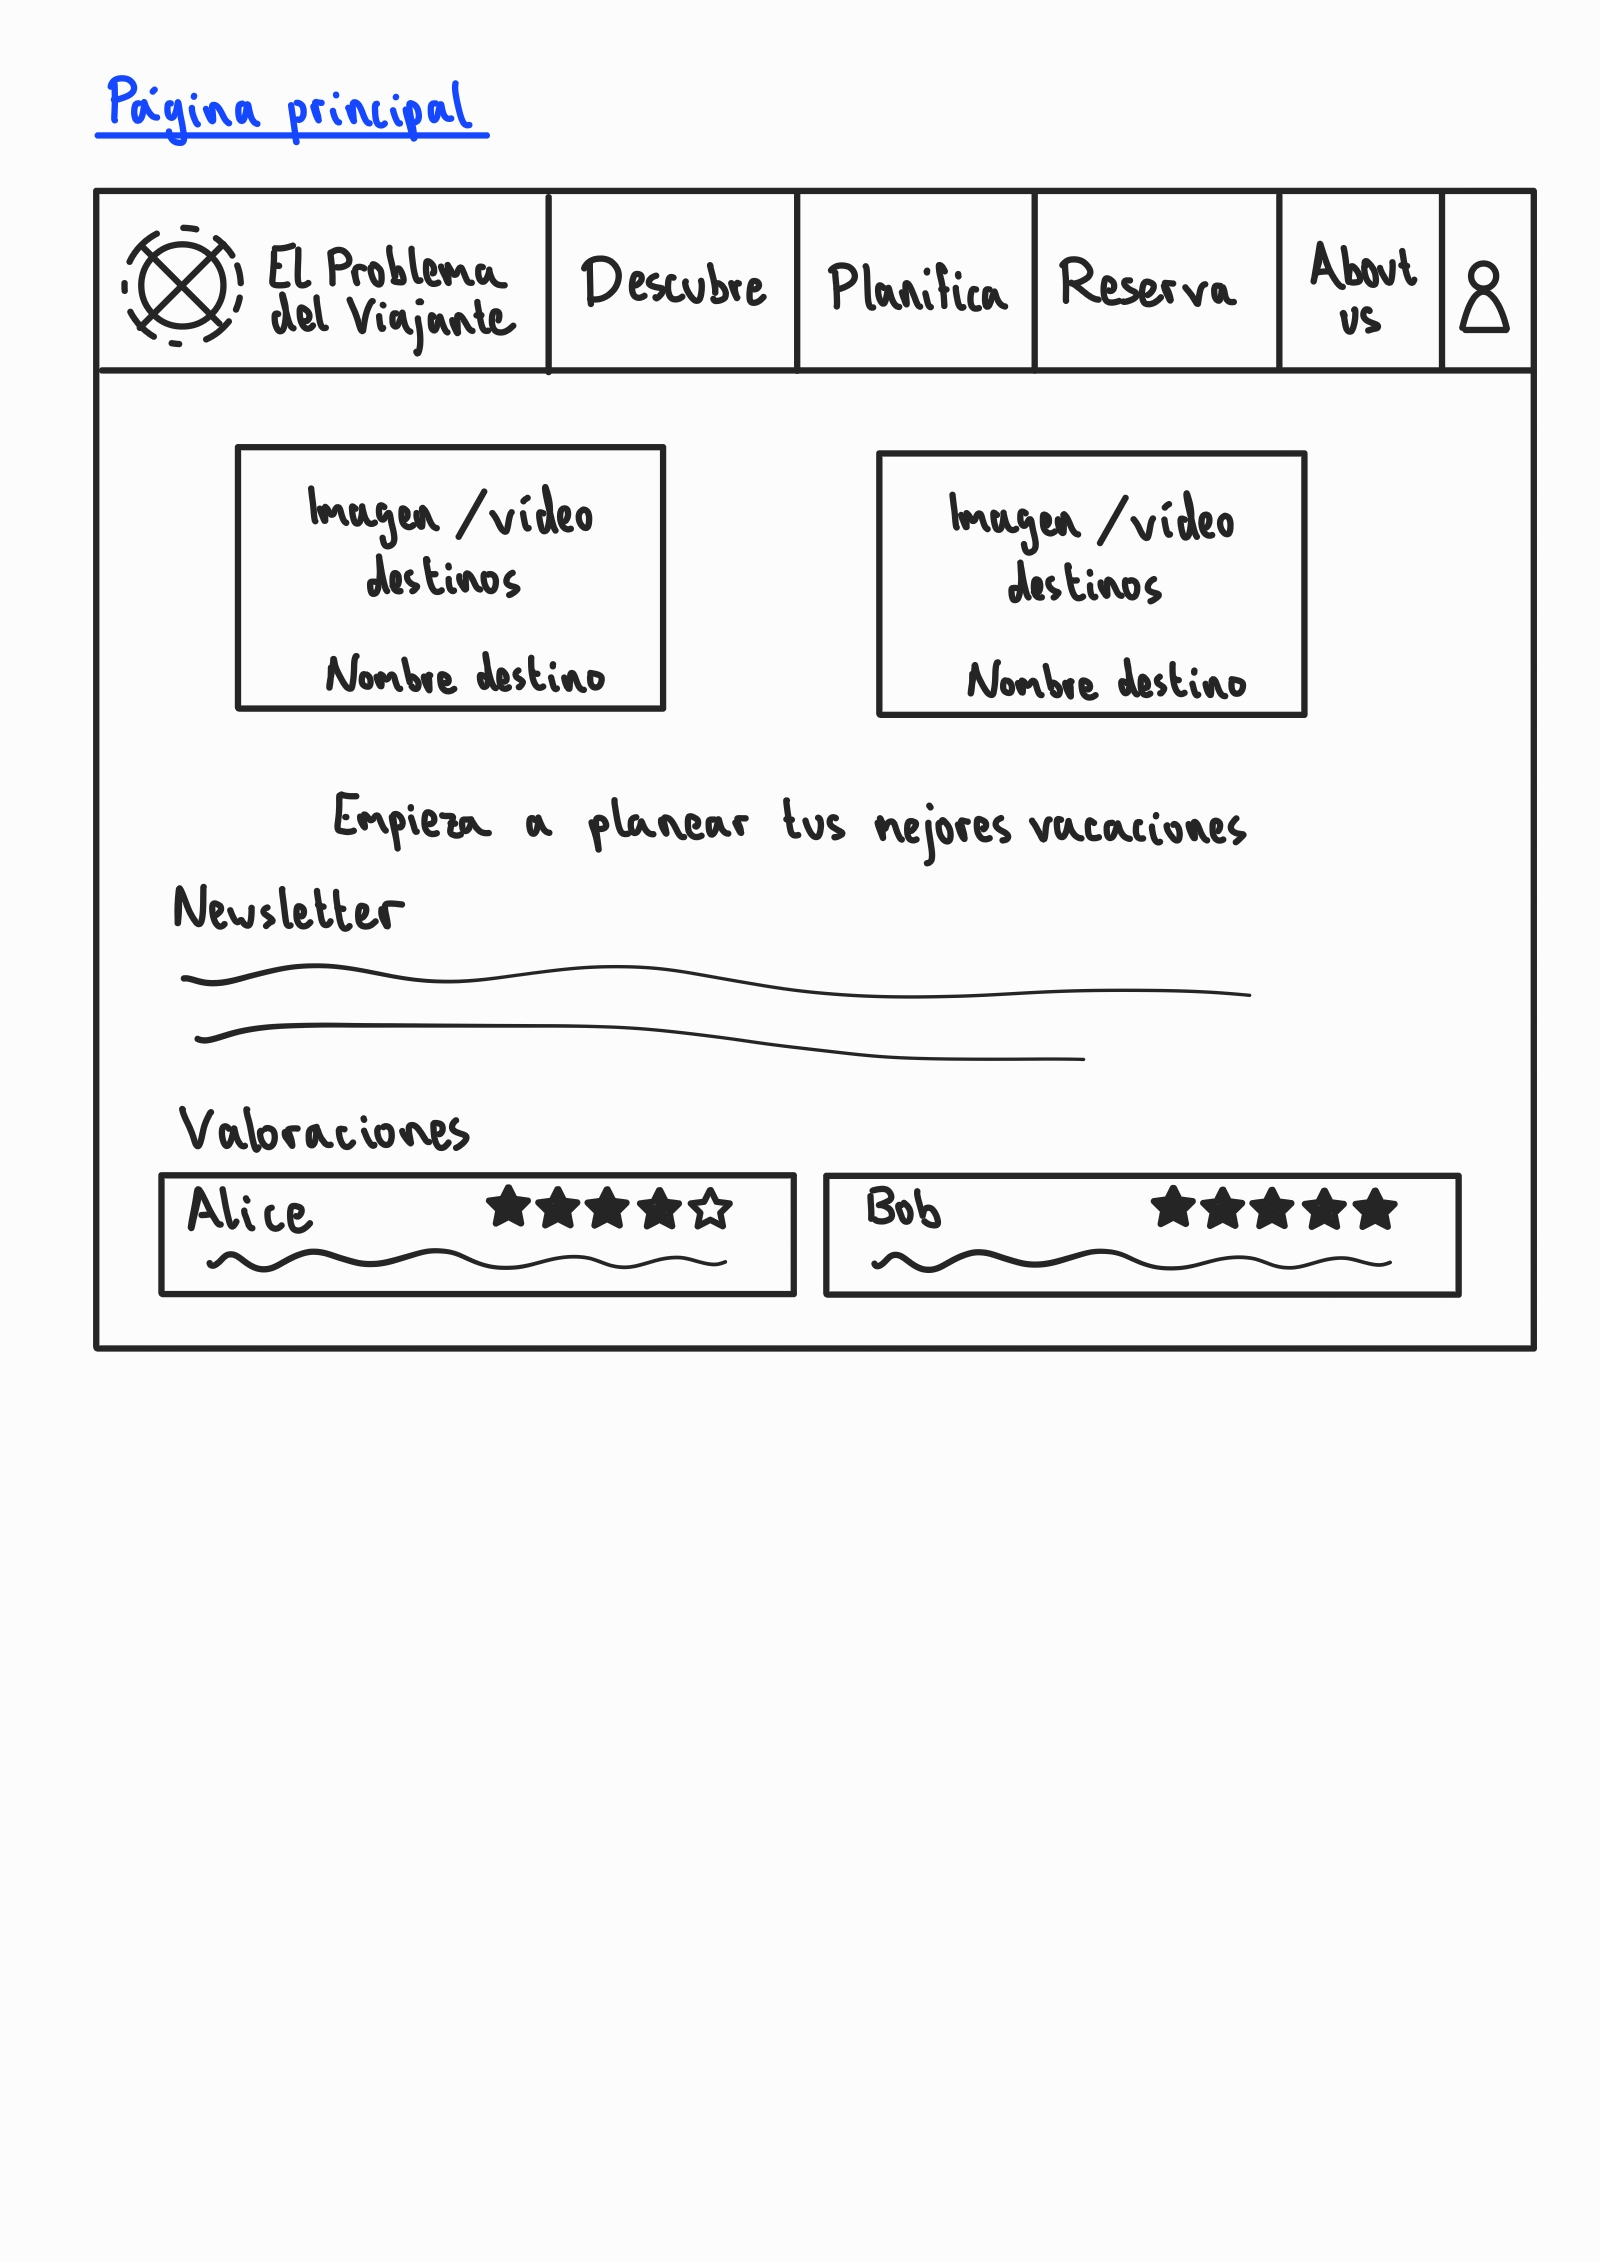
\includegraphics[width=\textwidth]{1-principal.jpg}
		\caption{Prototipo Página principal}
	\end{figure} 

	En esta figura se puede ver la \textbf{página principal} del sitio web. Aquí, se ve la barra de navegación global, que será común a todas las páginas, unos cuantos elementos visuales sobre algunos destinos destacados para captar la atención del visitante, un apartado de \textit{newsletter} con novedades importantes y una sección con valoraciones de clientes.
	
	Desde la barra de navegación, el usuario podrá registrarse por medio de correo electrónico para poder realizar valoraciones, que se guarden sus viajes, crear una planificación colaborativa y obtener mejores recomendaciones.
	
	\newpage
	
	\begin{figure} [H]
		\centering
		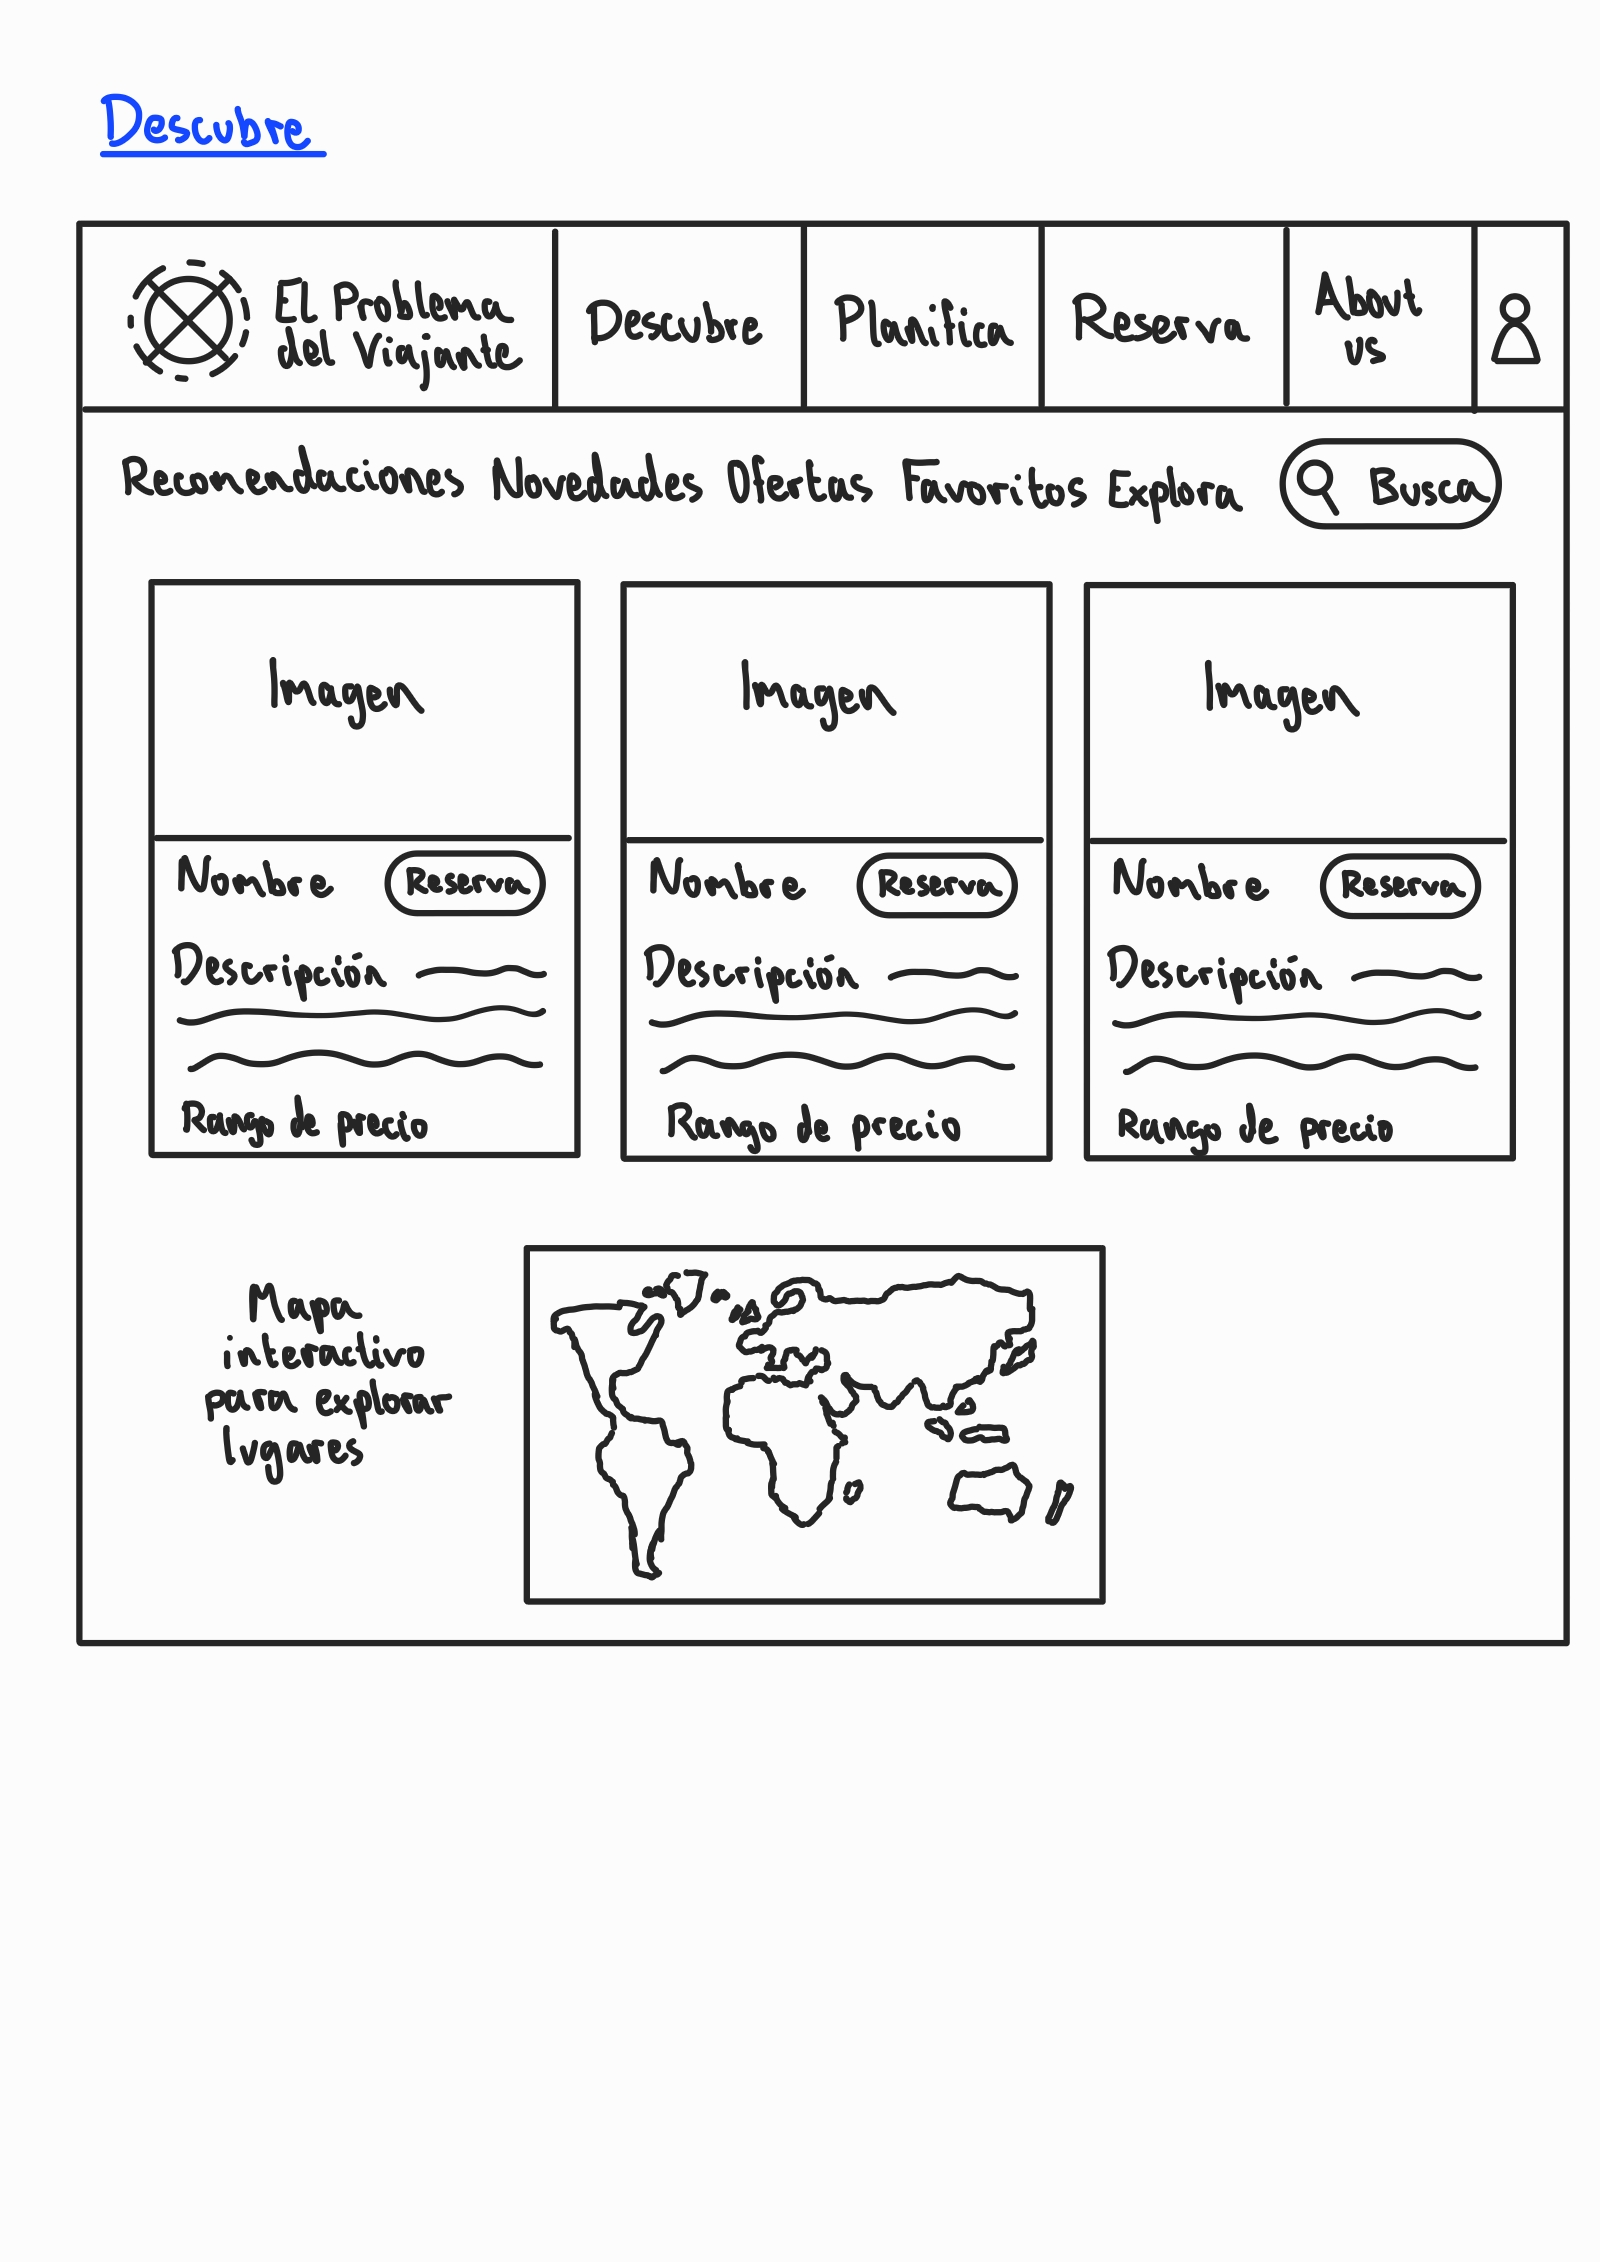
\includegraphics[width=\textwidth]{2-descubre.jpg}
		\caption{Prototipo Descubre}
	\end{figure} 

	En el apartado de \textbf{Descubre} se pretende que los clientes de la página que no tienen todavía claro cuál es el destino del viaje que quieren puedan explorar sus opciones. 
	
	Se ve, en primer lugar, una barra de navegación secundaria en la que aparecen diferentes subsecciones. En cada una de estas se presentarán destinos asociados al criterio empleado. En todas estas aparecerán diversos paquetes de viajes, mostrando imágenes y descripciones de los lugares a los que viajar. Asimismo, se incluye un mapa interactivo en el que aparecerán destacados los lugares mencionados en las tarjetas que aparecen en la página. Interactuando con este mapa, el cliente podrá, además, filtrar la búsqueda a un destino en concreto. Se incluyen además algunos destinos recomendados, consejos generales para la planificación de viajes y un apartado sobre la seguridad en las reservas.

	\newpage 
	
	\begin{figure} [H]
		\centering
		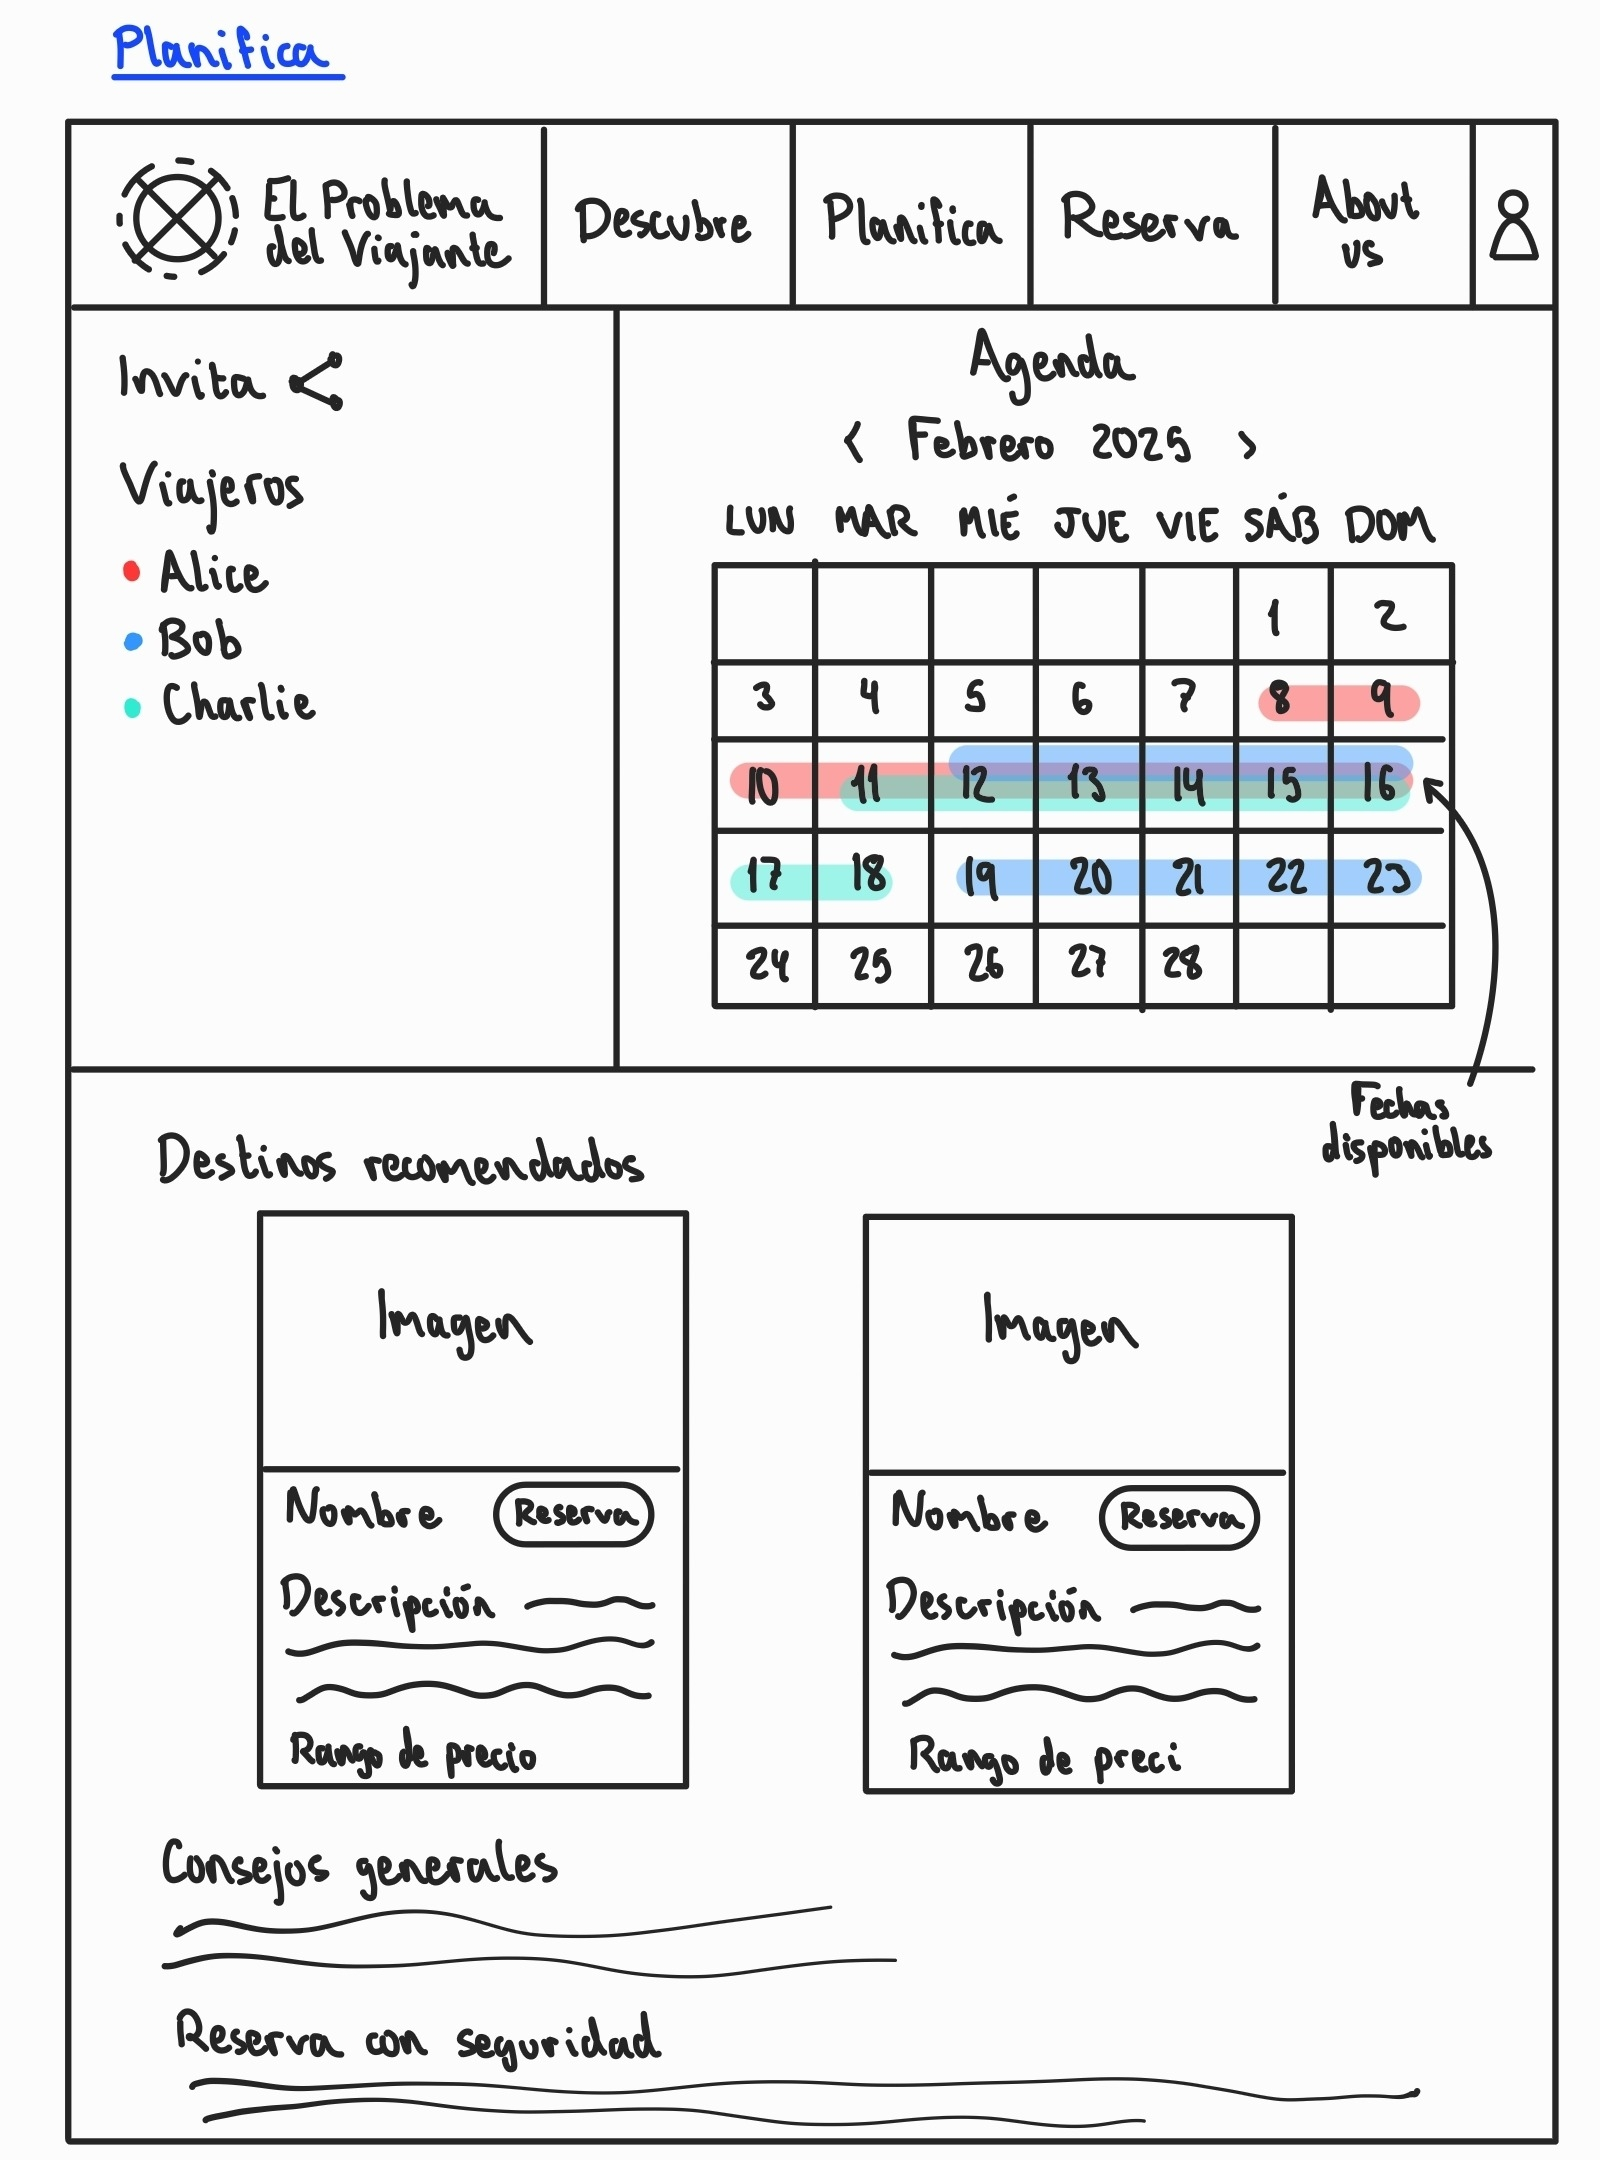
\includegraphics[width=\textwidth]{3-planifica.jpg}
		\caption{Prototipo Planifica}
	\end{figure} 

	En la sección de \textbf{Planifica}, el cliente podrá planificar su viaje con, posiblemente, otros usuarios. Así, están disponibles una columna en la que se puede invitar a otros viajeros y un calendario en el que cada uno de los participantes en un viaje puede marcar las fechas que tiene disponibles para una planificación más eficiente.

	\newpage
	
	\begin{figure} [H]
		\centering
		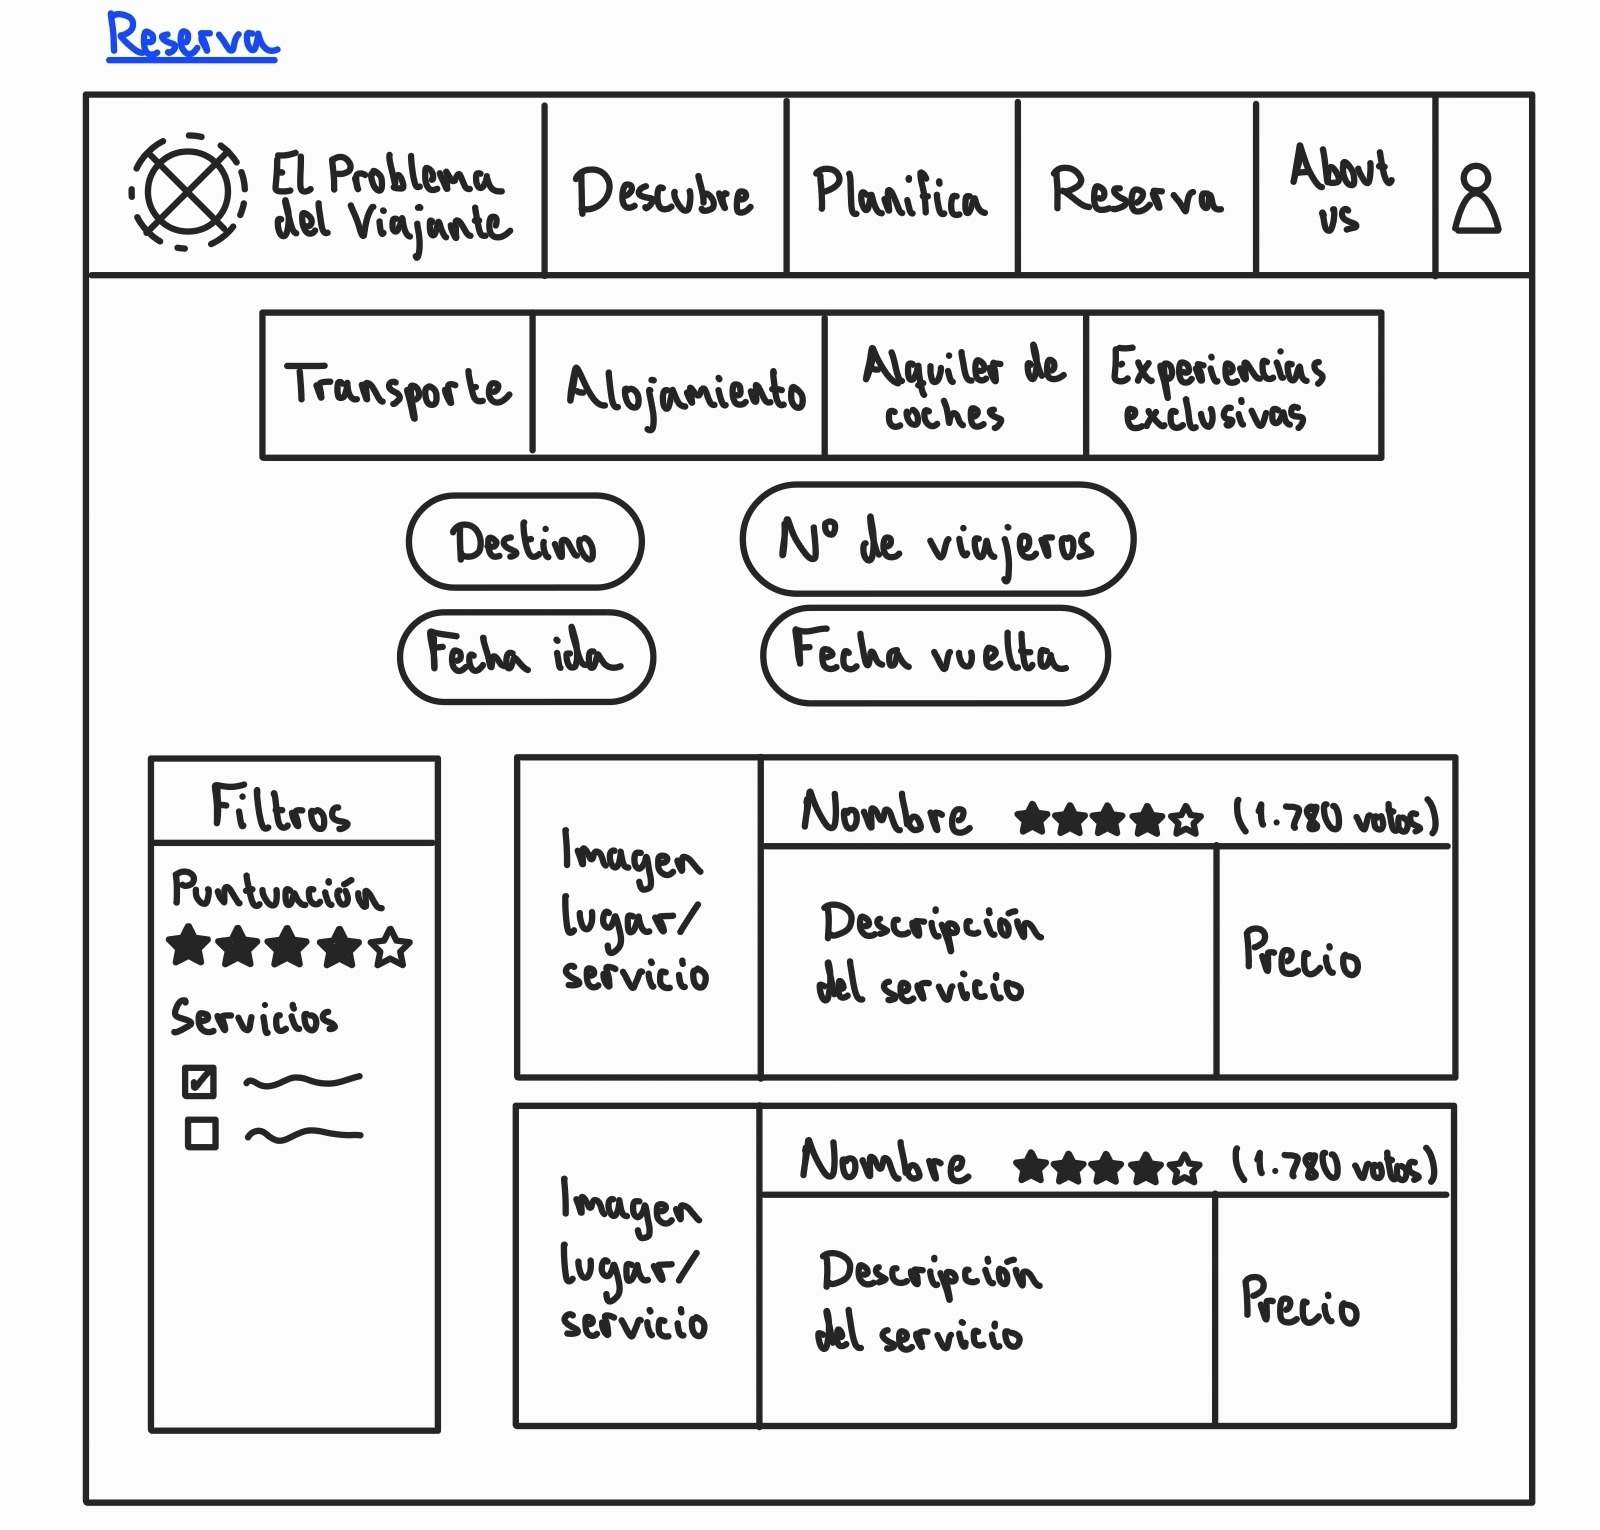
\includegraphics[width=\textwidth]{4-reserva.jpg}
		\caption{Prototipo Reserva}
	\end{figure} 

	En la página de \textbf{Reserva} el usuario podrá gestionar las reservas necesarias para su viaje. Estas incluyen el transporte hasta el lugar, alojamiento, alquiler de vehículos y otras experiencias exclusivas facilitadas por nuestro sitio web.
	
	Se incluye un filtro principal por destino, número de viajeros y fechas de ida y vuelta. Hay otros filtros secundarios que se podrán aplicar sobre la puntuación y el tipo de servicio. Una vez seleccionados estos campos, aparecerán los servicios recomendados por la web, con una imagen, su nombre, descripción y precio para que el usuario pueda gestionar su reserva.

	\newpage

	\begin{figure} [H]
		\centering
		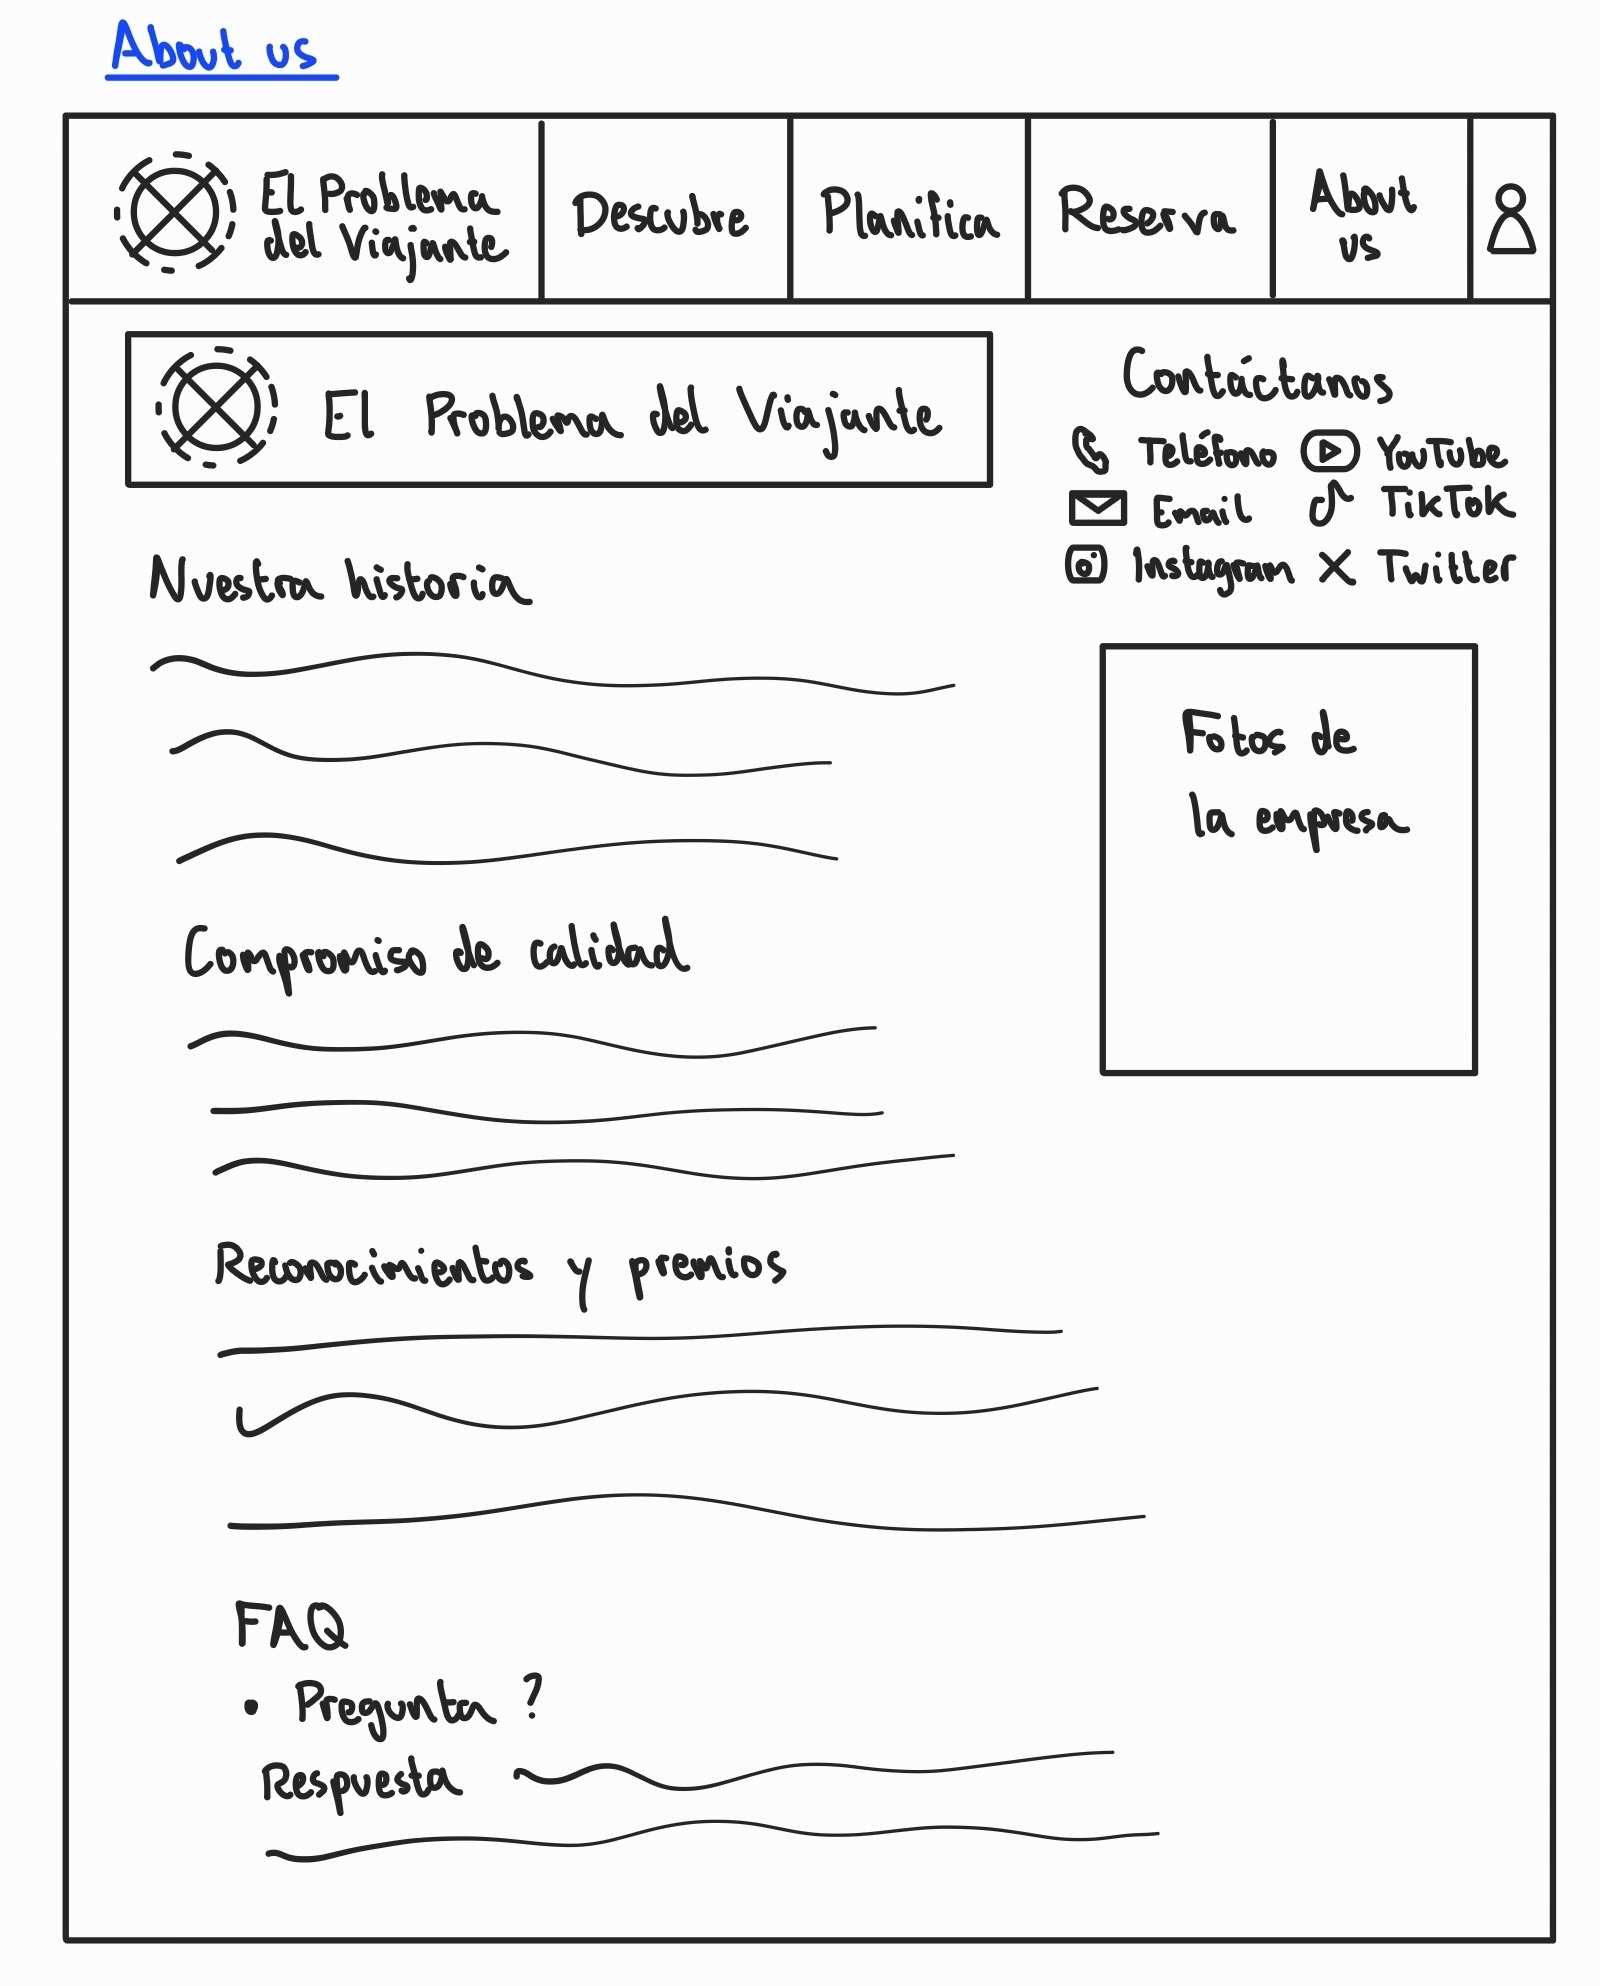
\includegraphics[width=\textwidth]{5-about_us.jpg}
		\caption{Prototipo Página principal}
	\end{figure} 

	La página de \textbf{About us} es principalmente de texto con información sobre la empresa ficticia. Hay información de contacto, la historia de la empresa, reconocimientos y premios, indicadores de calidad y preguntas frecuentes (FAQ).
	
	\newpage
	
	\subsection{Esqueleto digital}
	El \textit{wireframe} ayuda a establecer las proporciones entre los elementos de la página y a establecer la jerarquía de información del documento en términos de tamaño y posición. Para hacer el diseño, se ha utilizado el sitio web \href{https://figma.com}{Figma} está basado en la regla de las 12 columnas, en las que cada una de las páginas se divide verticalmente en 12 partes, el cual es un número suficientemente pequeño para ser fácilmente manejable (a diferencia de trabajar, por ejemplo, empleando píxeles) pero a la vez es lo suficientemente grande y tiene bastantes divisores como para permitir flexibilidad en el diseño. En los diseños que se muestran a continuación se marcan el número de columnas que ocupan los elementos destacados.
	
	Cabe destacar que para crear un diagrama con un tamaño razonable, todos los diagramas empleados se crearon en un tamaño equivalente a la resolución HD estándar (1920x1080 píxeles). Sin embargo, la expectativa de cualquier usuario de un sitio web es que las páginas admitan siempre desplazamiento en vertical para visualizar toda la información de la página. El desplazamiento en horizontal, si bien posible y utilizado, es menos habitual. Por este motivo, se representa el número de columnas pero no el de filas, y muchos de los elementos aparecen artificialmente distorsionados en la horizontal para poder entrar en el tamaño fijado, lo cual no se mantendrá en la página real.
	
	%\newpage
	
	\begin{figure} [H]
		\centering
		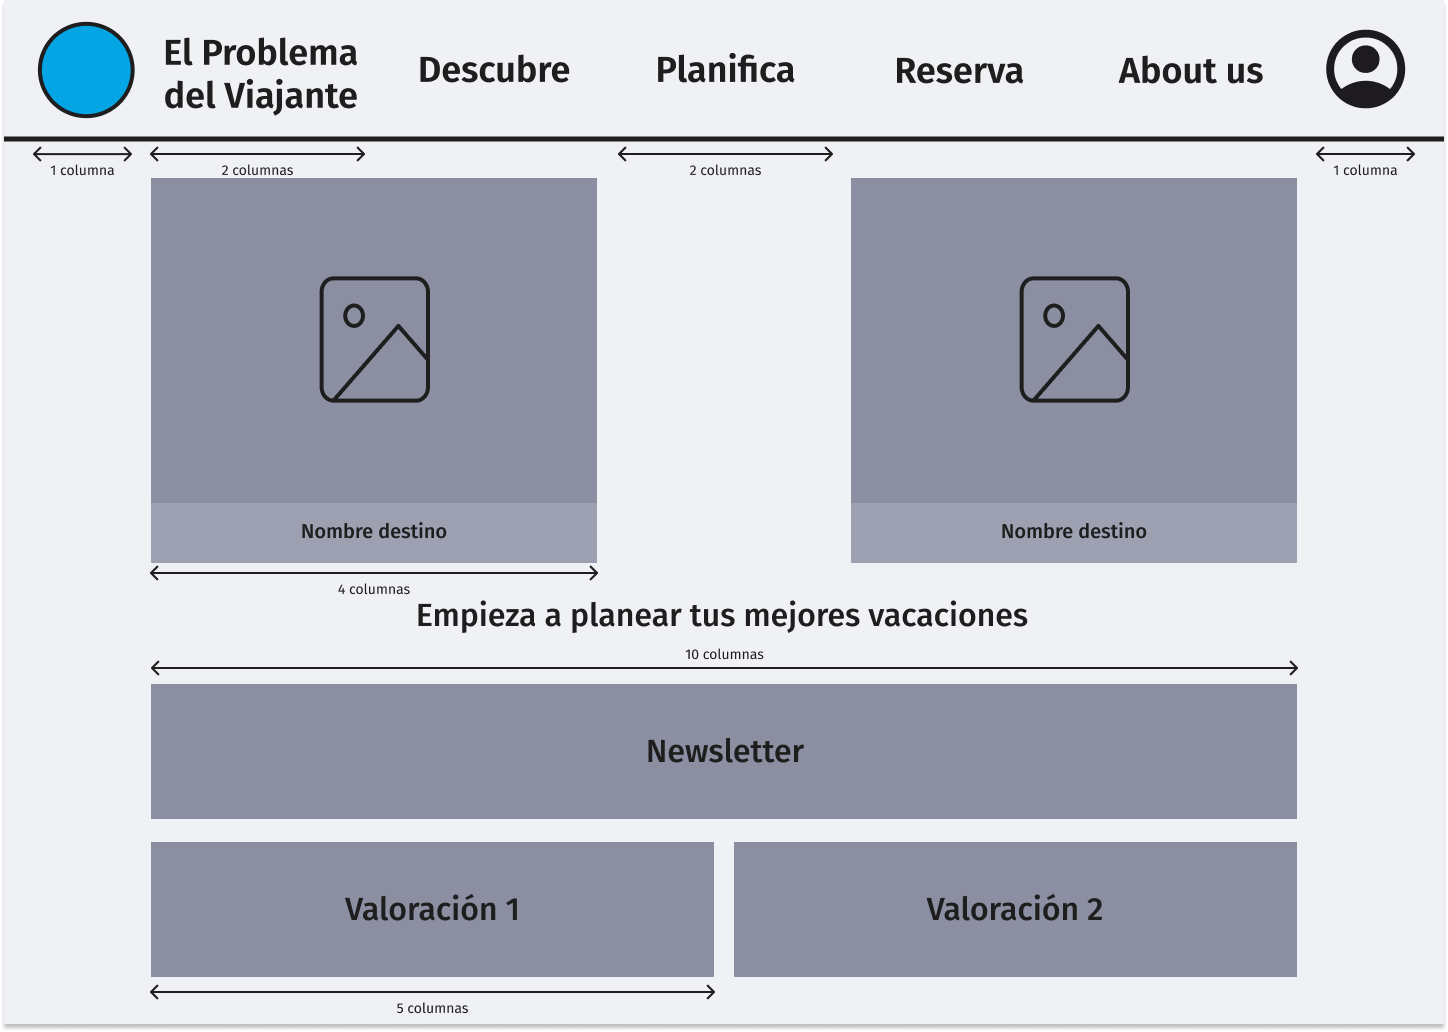
\includegraphics[width=\textwidth]{wireframe-principal.png}
		\caption{Wireframe Página principal}
	\end{figure} 

	Como se ha comentado, se muestran las columnas que ocupa cada elemento. Cabe destacar que la versión final para un dispositivo móvil diferirá significativamente respecto a la imagen mostrada, ya que habrá que tener en cuenta su orientación vertical, por lo que no se mostrarán diseños a dos columnas como este. Por otro lado, el \textit{newsletter} y las valoraciones no se verían completamente al ingresar en la página web, sino que habría que desplazarse verticalmente para visualizar su contenido.
	
	
	\begin{figure} [H]
		\centering
		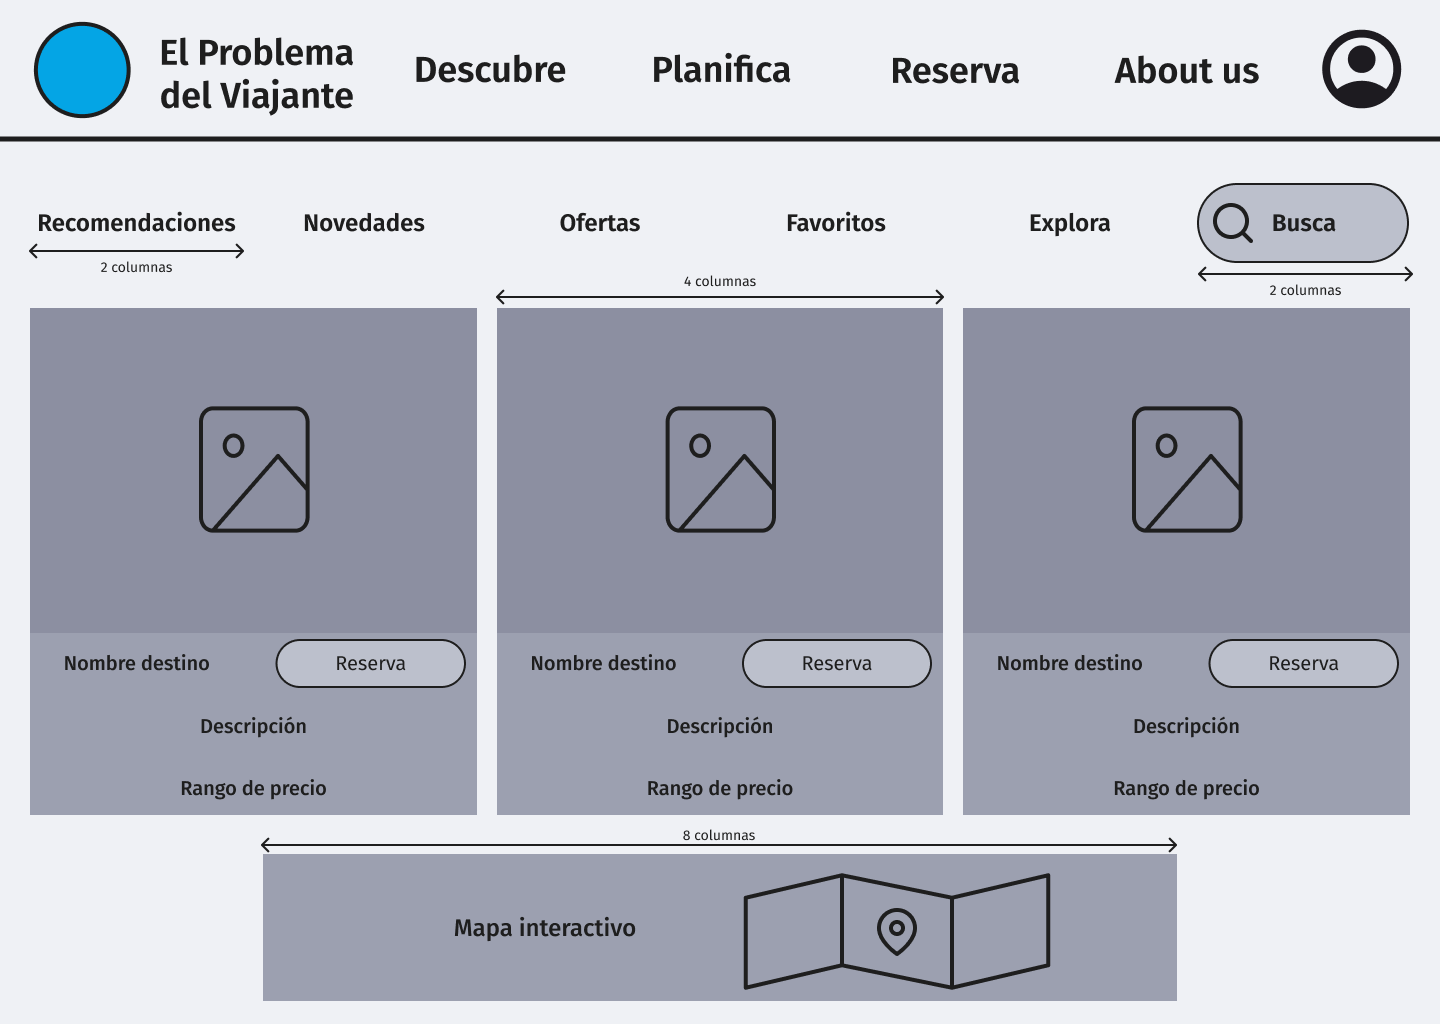
\includegraphics[width=\textwidth]{wireframe-descubre.png}
		\caption{Wireframe Descubre}
	\end{figure}

	En este caso se opta por un diseño a tres columnas, siguiendo la regla de los tercios, en el que las imágenes aparecerían en la parte central de pantalla, y habría una barra de navegación secundario para elegir diferentes formas de búsqueda. De nuevo, en la versión móvil, el diseño sería distinto.
	
	\newpage

	\begin{figure} [H]
		\centering
		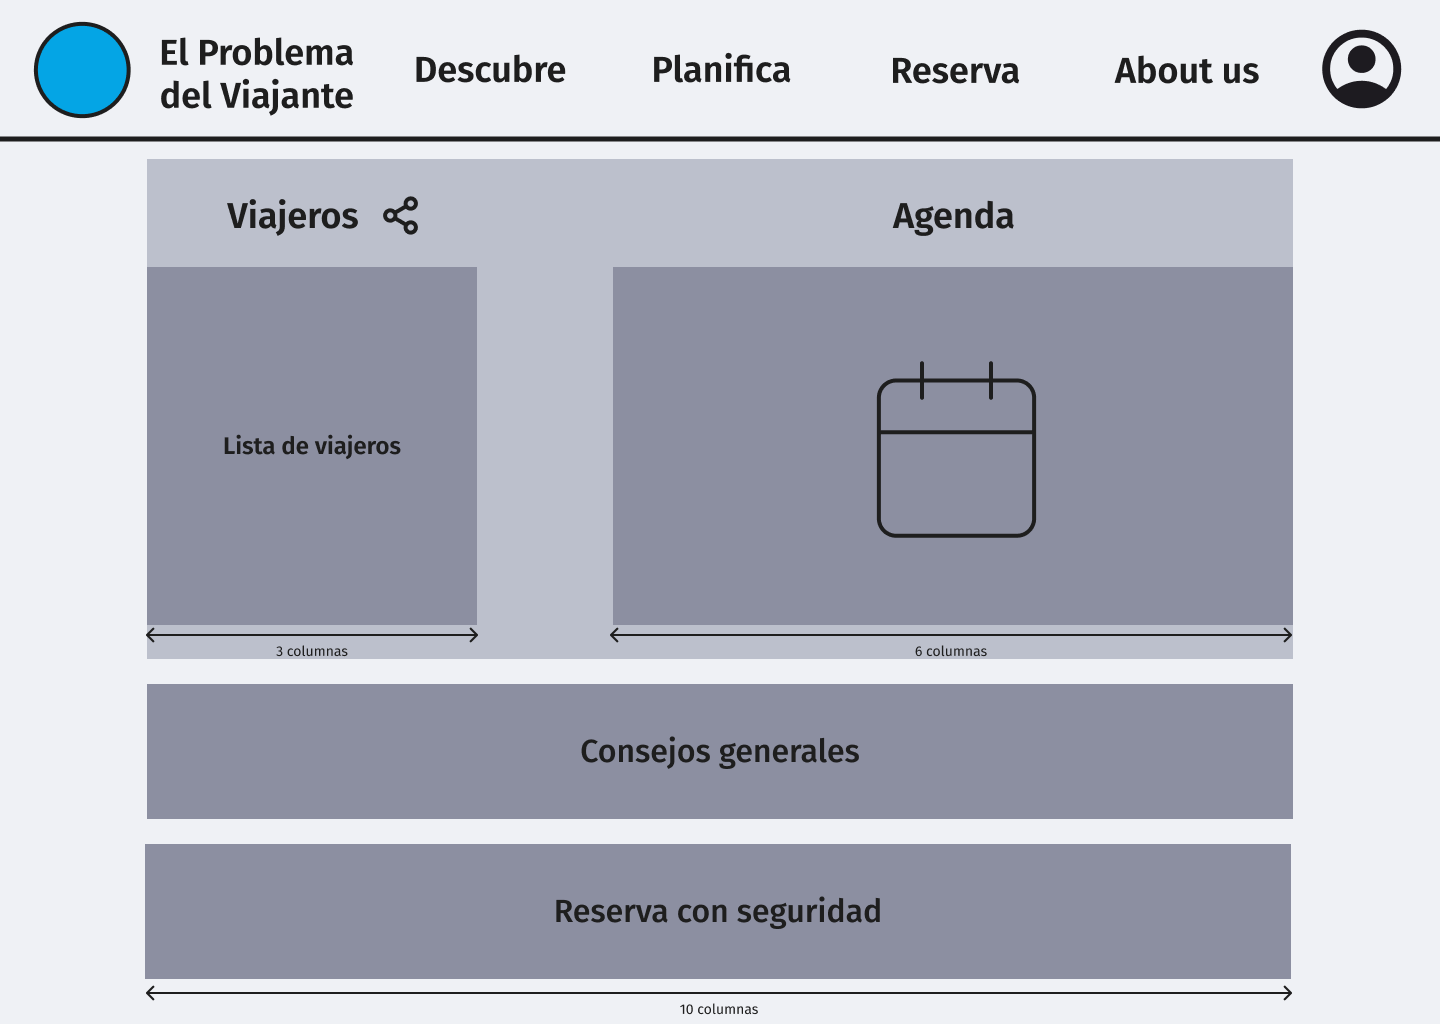
\includegraphics[width=\textwidth]{wireframe-planifica.png}
		\caption{Wireframe Planifica}
	\end{figure}

	En esta pestaña se muestra un calendario compartido por todos los viajeros que estén apuntados a un cierto viaje, junto a las fechas de salida y llegada, los lugares de visita reservados, etc. Más abajo, se encuentran consejos para los viajes, los cuales no se verían completamente en la forma final, ya que ocuparían más espacio del que aparece aquí.

	\newpage
	
	\begin{figure} [H]
		\centering
		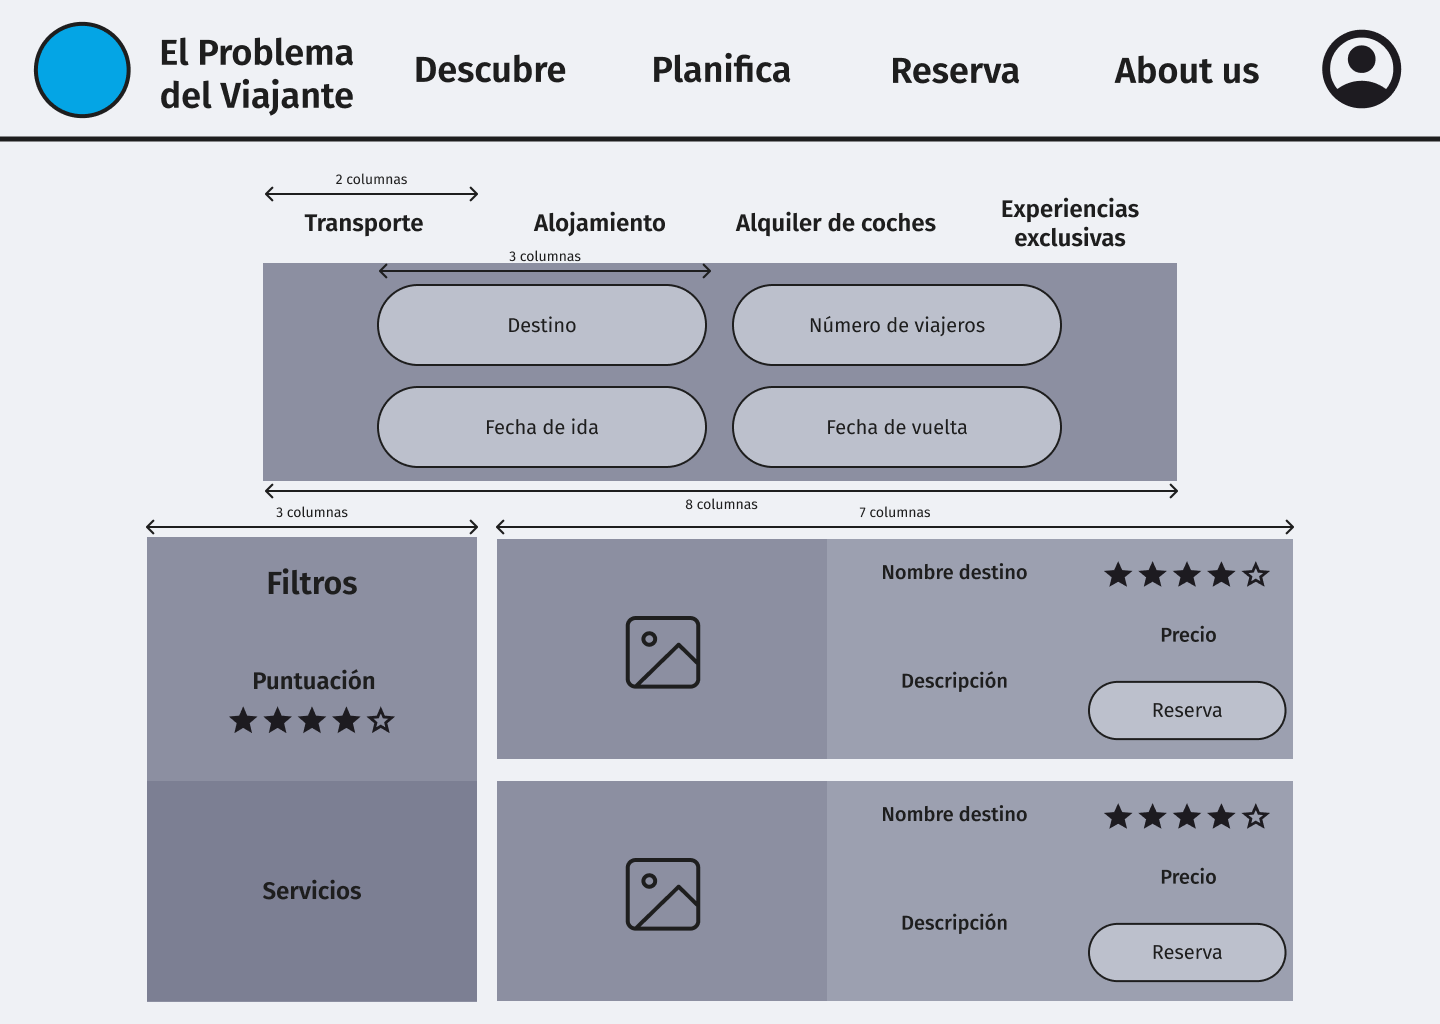
\includegraphics[width=\textwidth]{wireframe-reserva.png}
		\caption{Wireframe Reserva}
	\end{figure}

	En este wireframe se muestra otra barra de navegación secundaria diferente, con las diferentes modalidades de reserva, y múltiples opciones de personalización del viaje, desde la fecha hasta la puntuación y los servicios ofertados. El diseño está inspirado en el de las páginas web de reservas de viajes como \href{https://www.tripadvisor.es/Hotels-g186338-London_England-Hotels.html}{Tripadvisor}.
	
	\newpage
	
	\begin{figure} [H]
		\centering
		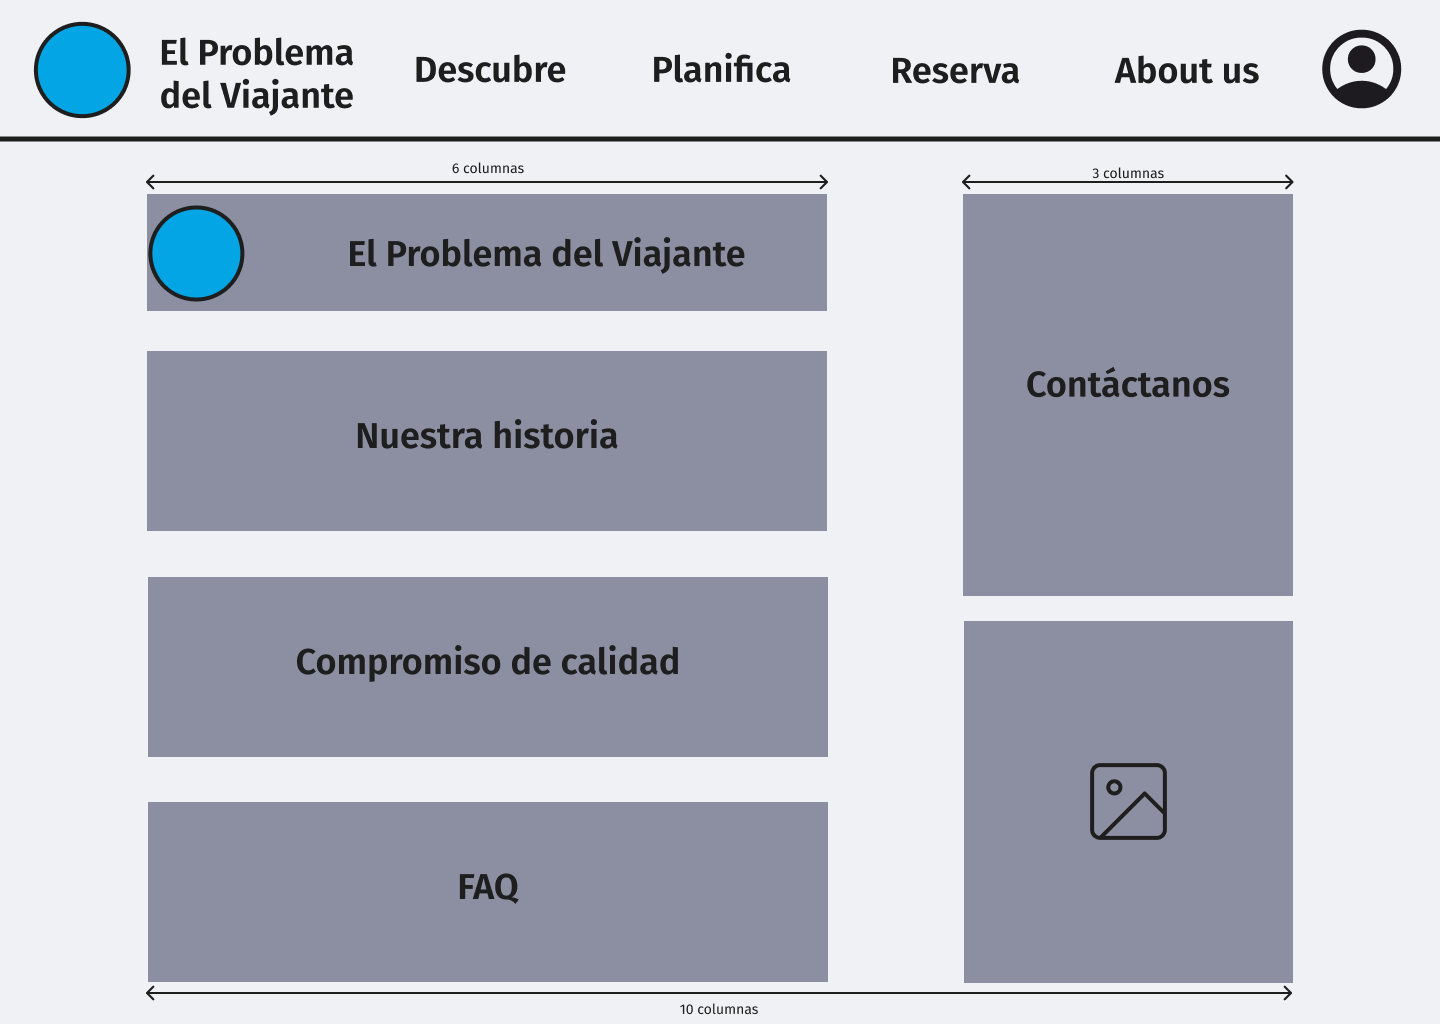
\includegraphics[width=\textwidth]{wireframe-about_us.png}
		\caption{Wireframe About us}
	\end{figure}
	
	Se opta por un diseño con una columna principal con los elementos más relevantes como la historia de la empresa, los indicadores de calidad y las preguntas frecuentes, y una columna secundario con las redes sociales y una imagen de los integrantes de la empresa.
	
	
	
	\subsection{Diseño final}
	El uso de \textit{mockups} permite ver la apariencia final de la página, incluyendo colores, fuentes de texto, logos e imágenes que acompañan al diseño y que hasta este momento se habían obviado. En cuanto la paleta de colores, se optó por usar una paleta ya creada y disponible de forma abierta: \href{https://github.com/catppuccin/catppuccin?tab=readme-ov-file#-palette}{Catppuccin Latte}, a la que se le han añadido algunos colores propios, reutilizados de otros proyectos.
	
	Como tipografía elegida se utilizará Helvetica. Debido a que no está disponible en la herramienta utilizada para el diseño final, se ha usado una letra similar, Fira Sans.
	
	No se añade una descripción a cada una de la imágenes, como se ha hecho en los dos apartados anteriores, ya que muestran la misma disposición del contenido que los \textit{wireframes}, añadiendo los respectivos colores y formateos de texto.
	
	\begin{figure} [H]
		\centering
		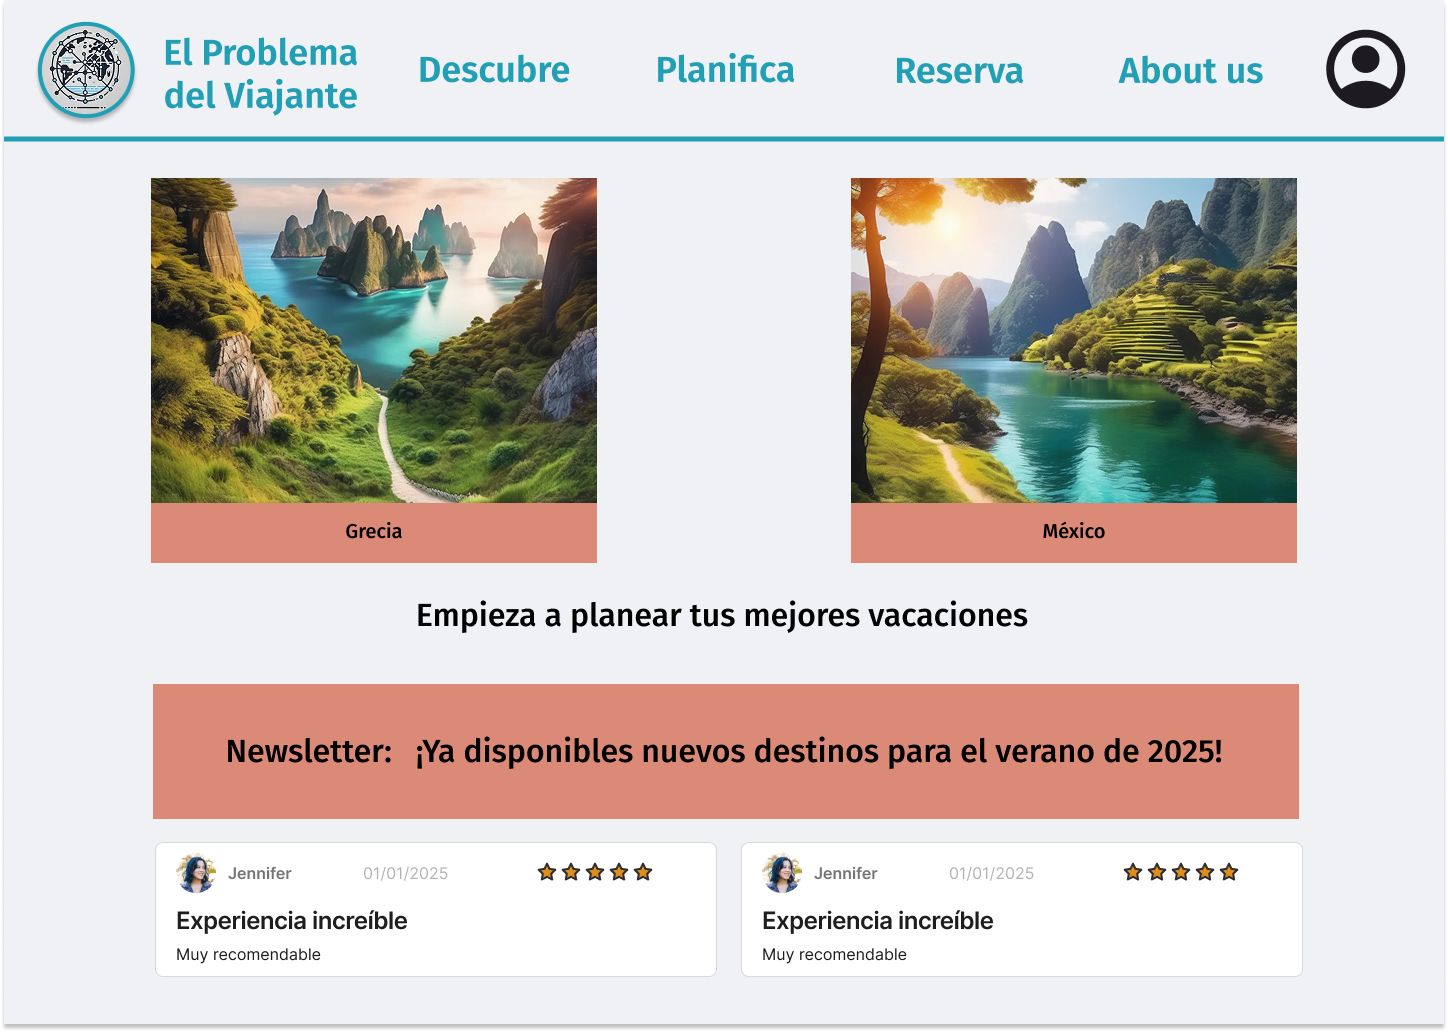
\includegraphics[width=\textwidth]{mockup-principal.png}
		\caption{Mockup Página principal}
	\end{figure}

	\begin{figure} [H]
		\centering
		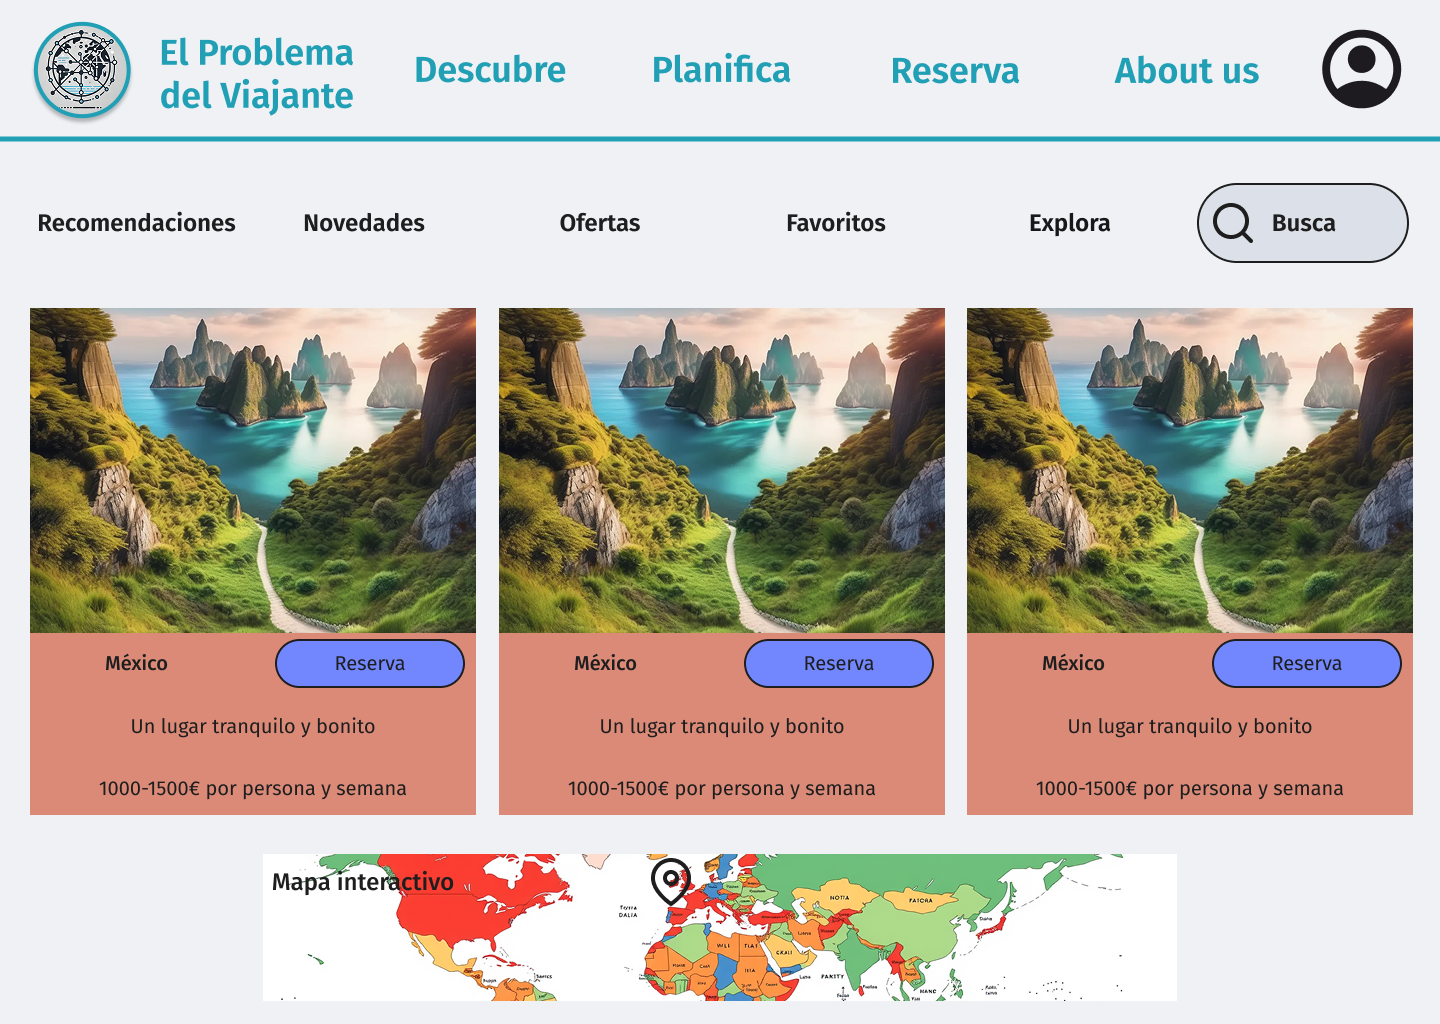
\includegraphics[width=\textwidth]{mockup-descubre.png}
		\caption{Mockup Descubre}
	\end{figure}
	
	\begin{figure} [H]
		\centering
		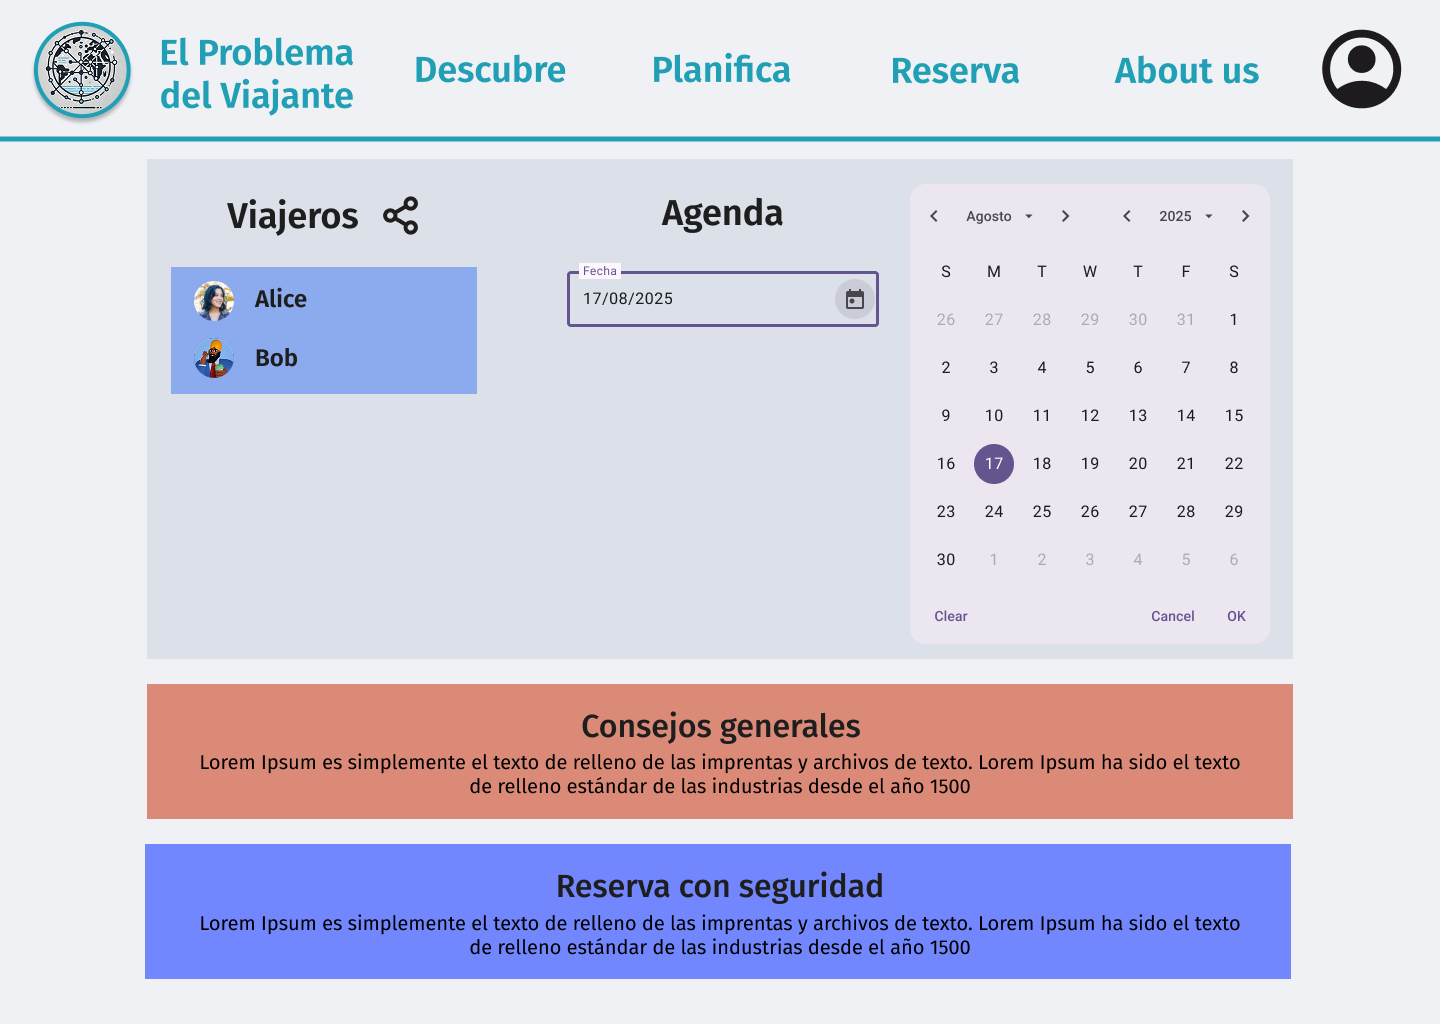
\includegraphics[width=\textwidth]{mockup-planifica.png}
		\caption{Mockup Planifica}
	\end{figure}
	
	\begin{figure} [H]
		\centering
		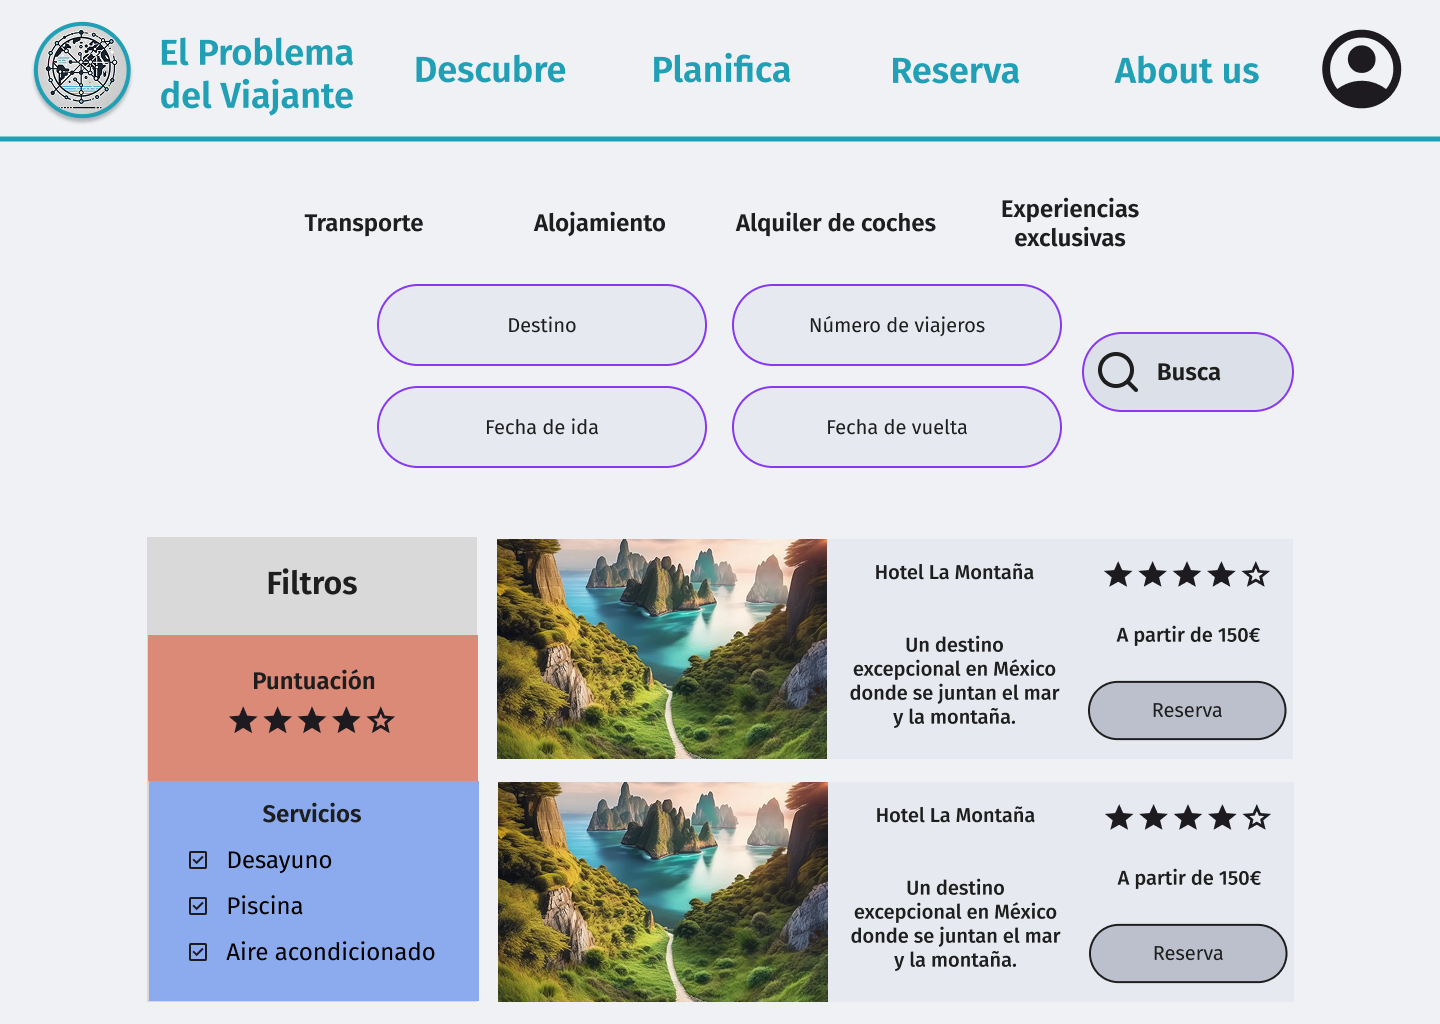
\includegraphics[width=\textwidth]{mockup-reserva.png}
		\caption{Mockup Reserva}
	\end{figure}
	
	\begin{figure} [H]
		\centering
		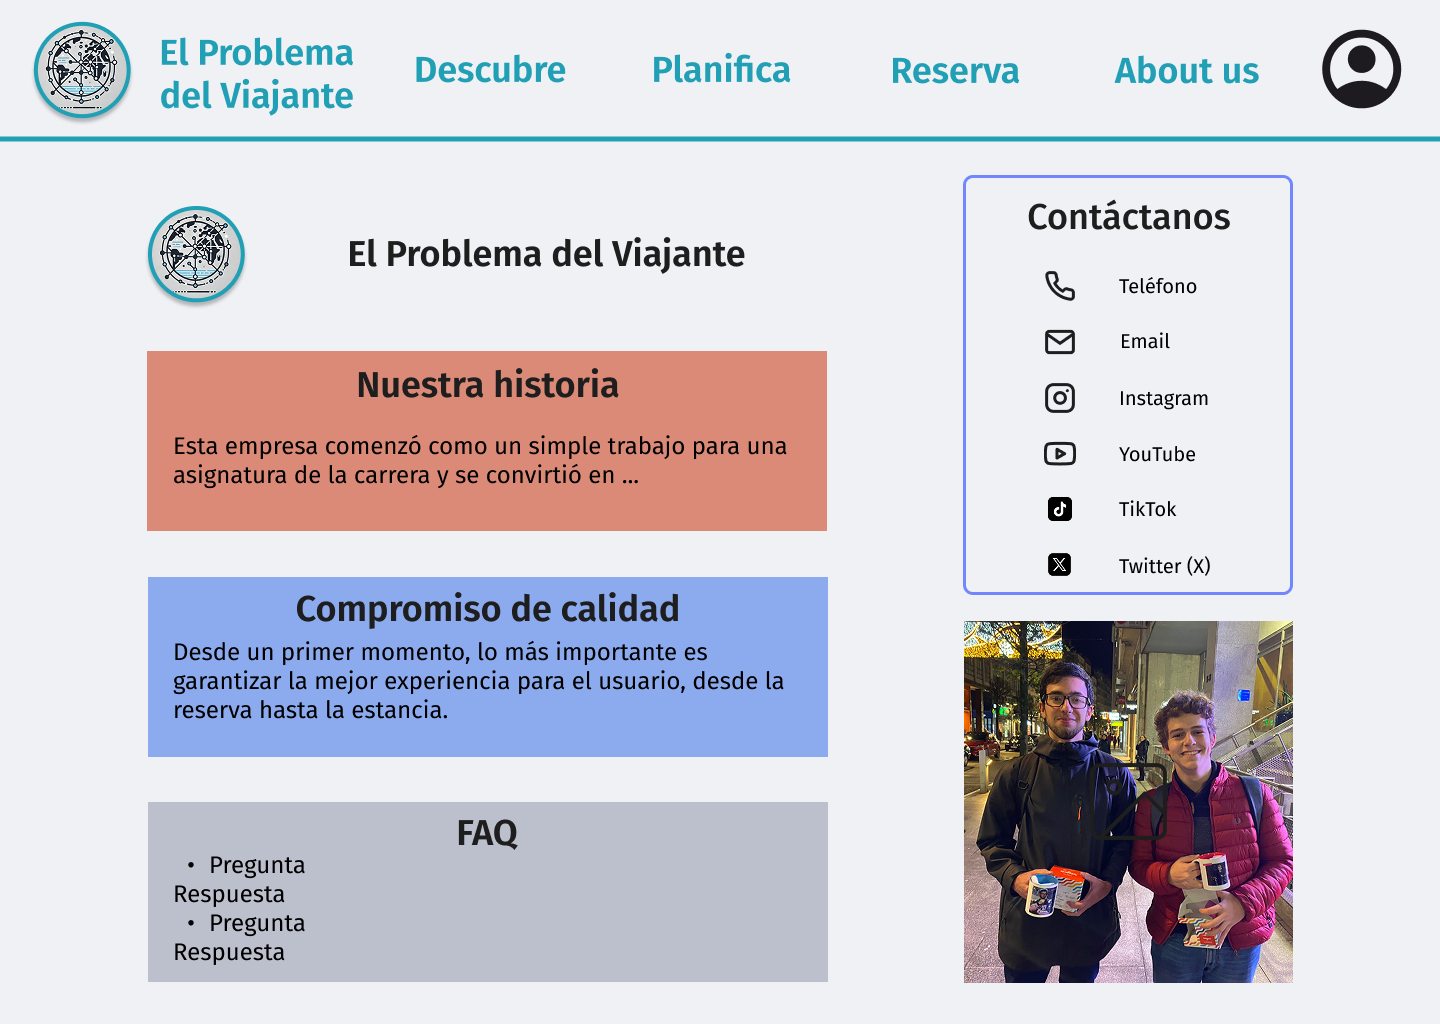
\includegraphics[width=\textwidth]{mockup-about_us.png}
		\caption{Mockup About us}
	\end{figure}


	\newpage
	\section{Storyboard}
	El \textit{storyboard} permite visualizar de forma dinámica el sitio web. Esto permite ilustrar cómo interaccionan elementos y colores, cómo funciona el sistema de navegación propuesto y, en general, tener una idea de si el sitio web representa aquello para lo que fue diseñado.
	
	Para ello, se añade información sobre los diseños finales del apartado anterior, donde se muestra cómo interactuar con los elementos de la página. A continuación se muestran tres casos de uso.
	
	\begin{figure} [H]
		\centering
		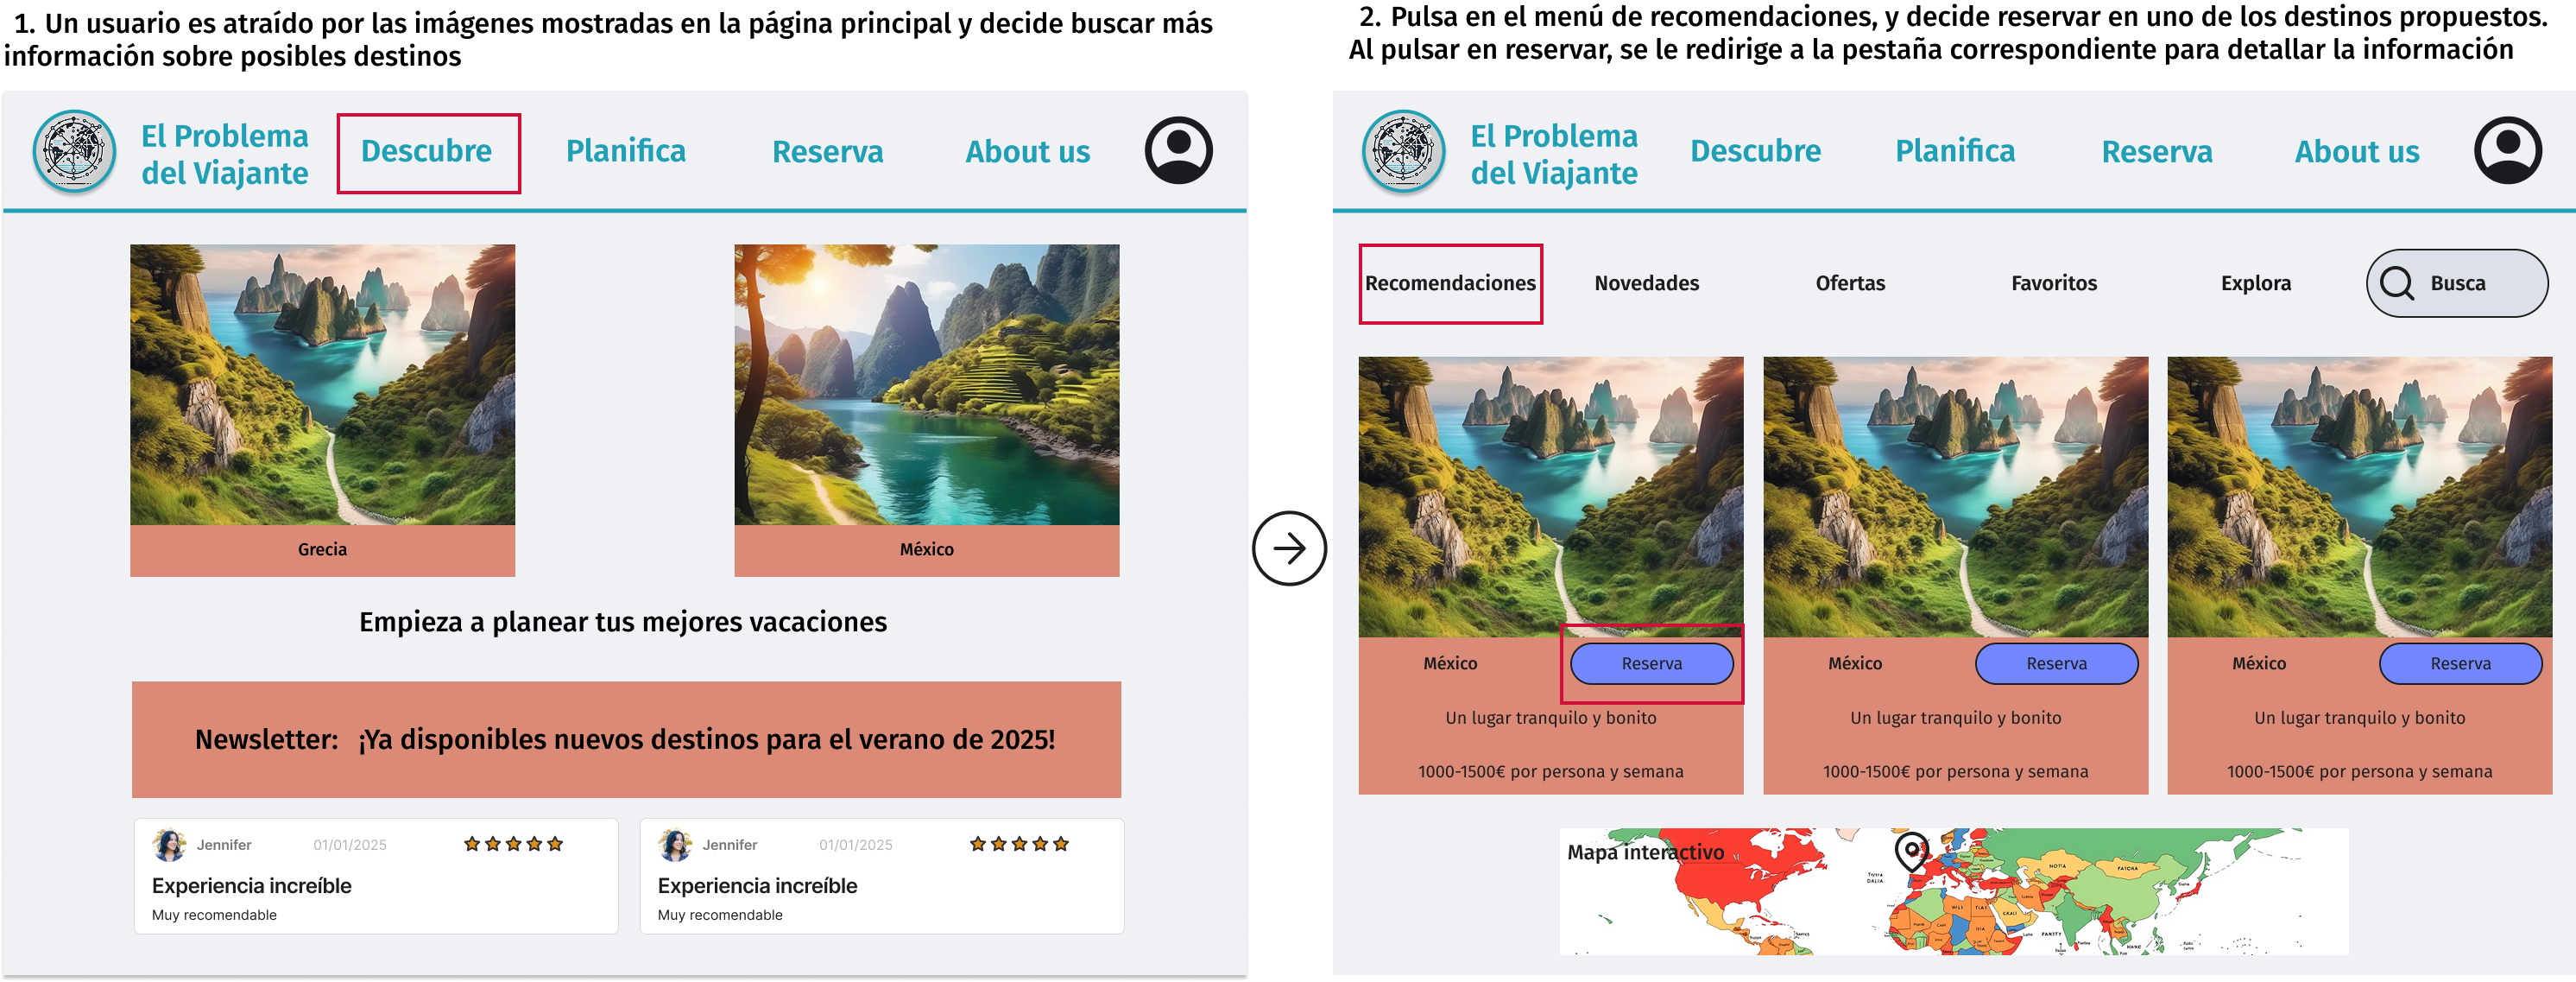
\includegraphics[width=\textwidth]{storyboard-descubrir.png}
		\caption{Storyboard Descubre}
	\end{figure}

	Supongamos que el usuario accede a la página web ya que tiene interés en buscar posibles lugares de visita. Lo intuitivo sería pulsar en la pestaña de \textbf{Descubre} del menú de navegación. En ella, hay diferentes opciones en la barra de navegación secundaria, donde la más relevante sea posiblemente \textbf{Recomendaciones}, y en esta se mostrarán los destinos propuestos. Al pasar el ratón por encima de uno de ellos, el mapa se situará en el lugar donde se encuentran, para facilitar buscar información sobre sus alrededores. Por último, si decidiese que está interesado en hacer la reserva, al pulsar en el correspondiente botón se le redirigiría a la página web desde la que puede reservar.

	\begin{figure} [H]
		\centering
		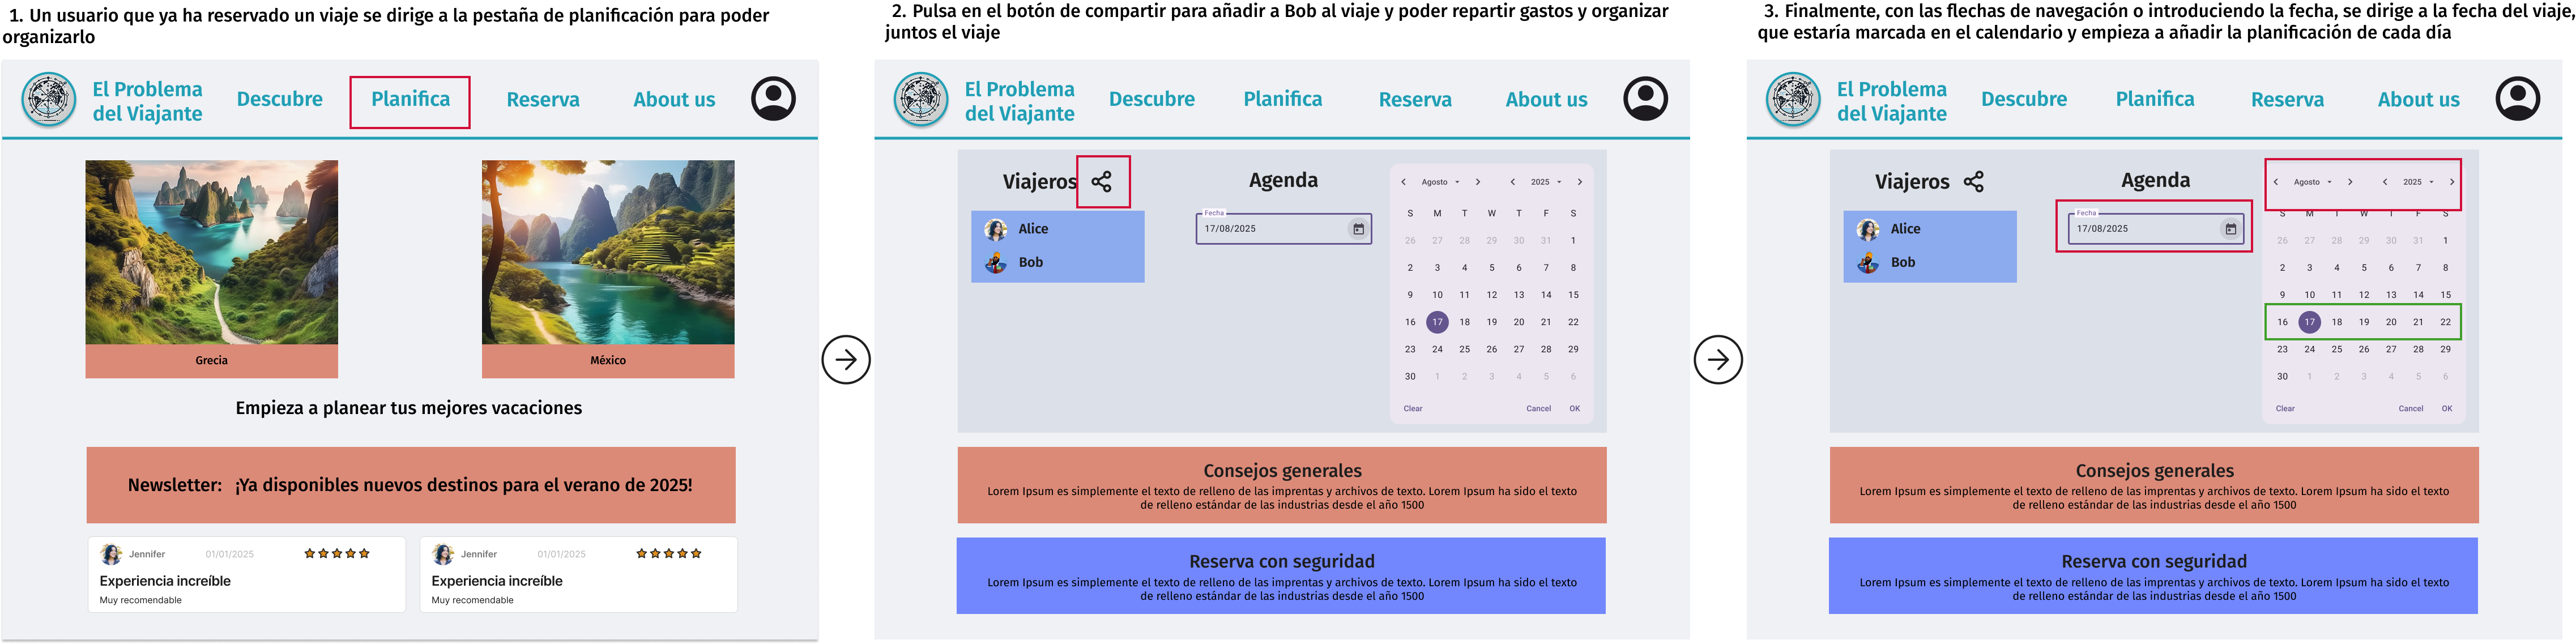
\includegraphics[width=\textwidth]{storyboard-planificar.png}
		\caption{Storyboard Planifica}
	\end{figure}

	\textcolor{red}{La imagen no se ve muy bien, igual hay que pasarla a vertical}
	
	Supongamos ahora que este mismo usuario, tras reservar un viaje y crearse una cuenta en la página web, decide comprobar las fechas de su reserva. Para ello, se dirige a la pestaña de \textbf{Planifica}, desde la que puede añadir a las personas que viajarán con él, lo cual facilita la organización del viaje, la elección de los lugares de visita y el reparto de gastos, además de asegurar que no habrá actividades que se superpongan.
	
	Asimismo, pulsando en el calendario puede cambiar el mes en el que se encuentra y añadir la planificación de cada día según corresponda.
	
	\begin{figure} [H]
		\centering
		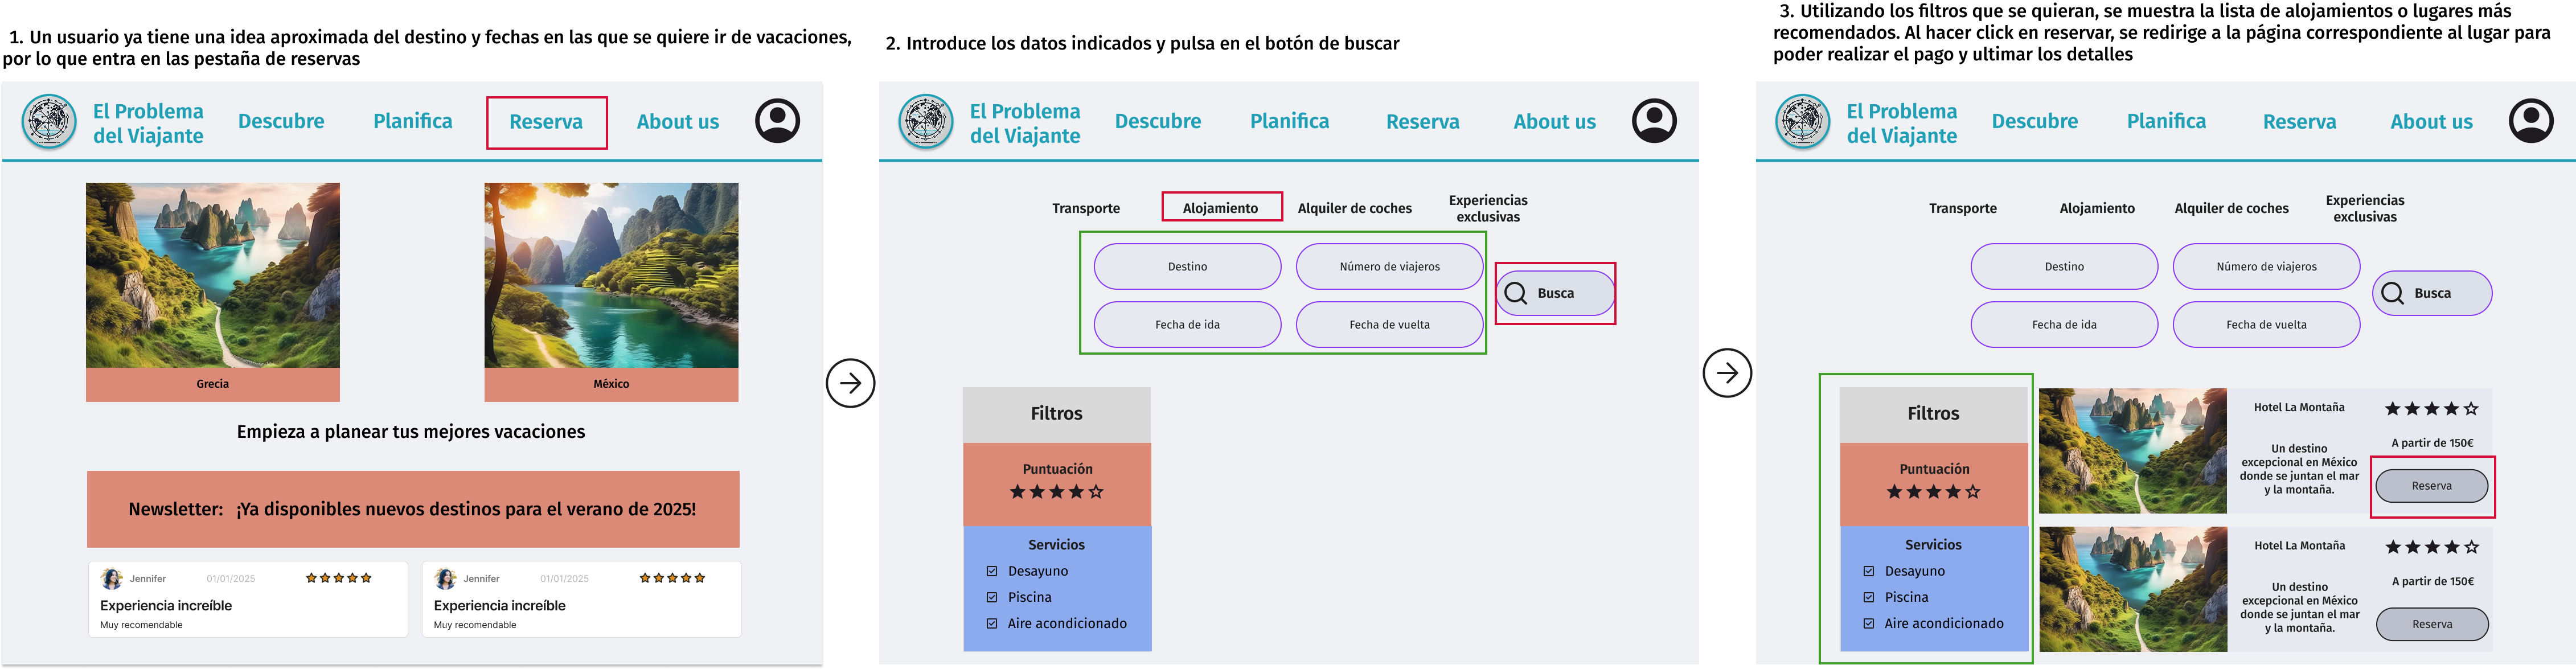
\includegraphics[width=\textwidth]{storyboard-reservar.png}
		\caption{Storyboard Reserva}
	\end{figure}

	Para el último, pensemos en otro usuario que sí tiene claro el destino al que quiere ir, pero no dónde se va a alojar, por lo que accede a la pestaña de \textbf{Reserva}, desde donde podrá ver diferentes ofertas. En la barra de navegación secundaria, selecciona \textbf{Alojamiento} e introduce los datos necesarios, como la fecha ida y de vuelta, y el nombre del destino.
	
	Al pulsar en buscar, se le mostrarán diferentes opciones, ordenadas según los filtro seleccionados, los cuales pueden modificarse para mostrar únicamente alojamientos con una puntuación superior a una dada, o que ofrezcan ciertos servicios como piscina o gimnasio. A continuación, si desea realizar la reserva mostrada, solamente tiene que pulsar en el correspondiente botón, el cual le redirigiría a la página web desde la que puede reservar.


	
	
	
	\section{Estructura de ficheros}
	\label{ficheros}
	Para la organización de los ficheros del proyecto, optamos por una estructura simple en directorios en la que el documento principal, 'index.html', está por sí solo en el nivel raíz, pues es lo que espera el servidor web. 
	
	Por otra parte, tenemos un directorio con la documentación en el que se incluye este documento y sus imágenes asociadas en su correspondiente subdirectorio, así como otros elementos de documentación que puedan surgir en el futuro.
	
	Para los contenidos en sí de la página web, disponemos de cuatro subdirectorios. Uno está destinado a almacenar todas las imágenes que serán necesarias para la elaboración del sitio web. Por otra parte, disponemos de una carpeta en la que se almacenarán los documentos HTML que darán estructura a las diferentes páginas. En el directorio de estilos se almacenarán los ficheros de CSS necesarios para dotar al sitio web de una apariencia profesional y consistente. Por último en el directorio de scripts se incluirán los ficheros de JavaScript que doten al sitio web de funcionalidades dinámicas. 
	
	\begin{figure} [H]
		\centering
		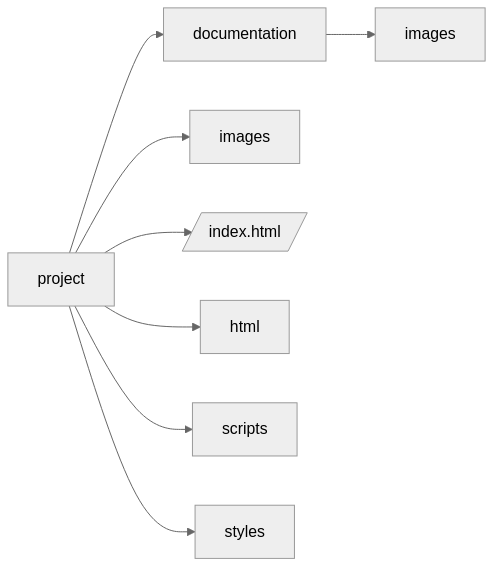
\includegraphics[width=0.8\textwidth]{estructura_ficheros.png}
		\caption{Diagrama de la estructura de ficheros}
	\end{figure}
	
	
	
	
	
	
	
	
	
	% ----------------------------------------------------------------------------
	% ----------------------------------------------------------------------------
	
	\chapter{Documentación HTML}
	
	En la siguiente parte del proyecto, se empieza a codificar el código HTML de las páginas, centrándose en el uso adecuado de las etiquetas HTML, siguiendo los estándares de \href{https://html.spec.whatwg.org/multipage/}{W3C}, y de momento no se codifican características de visualización de la página, pues corresponden a la parte de hojas de estilo. 
	
	Para cada una de las cinco página principales, se muestra a continuación los nombres de los elementos más importantes y en algunos casos sus mapas de etiquetas. Como se ha comentado en clase, solo se incluyen los mapas de etiquetas de los elementos con mayor contenido y dificultad, obviando así muchos que están formados únicamente por un encabezado y varios párrafos.
	

	\begin{figure} [H]
		\centering
		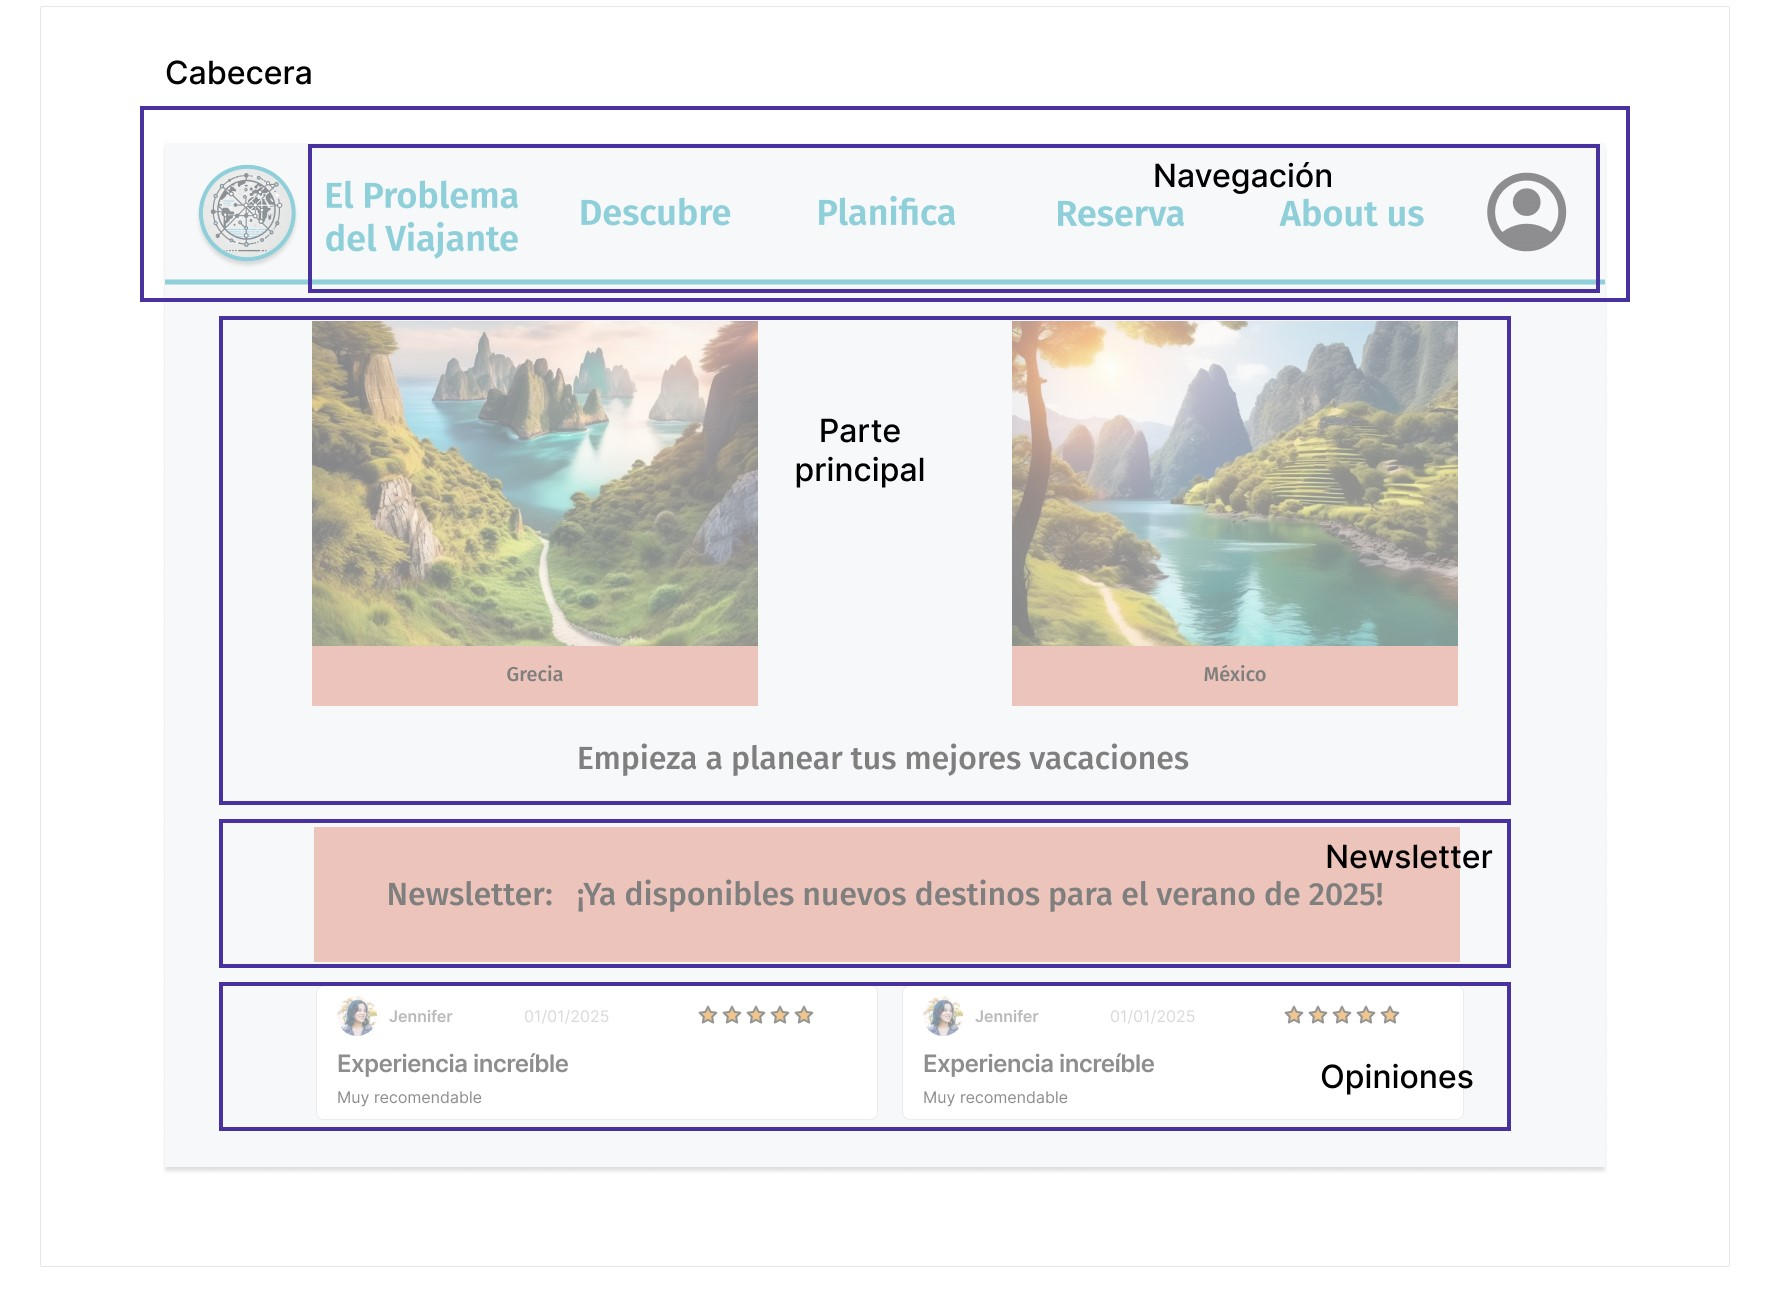
\includegraphics[width=\textwidth]{HTML/Doc-principal.jpg}
		\caption{Elementos página principal}
	\end{figure}

	En primer lugar, se va a comentar la barra de navegación, que es común a todos los elementos. Es sencilla, con el logo de la empresa, y con cinco apartados que nos redirigen precisamente a las cinco páginas principales de la web. Lo más relevante son las imágenes de la zona principal, ya que es lo primero que verá un usuario al ingresar en la página. 
	
	\begin{figure} [H]
		\centering
		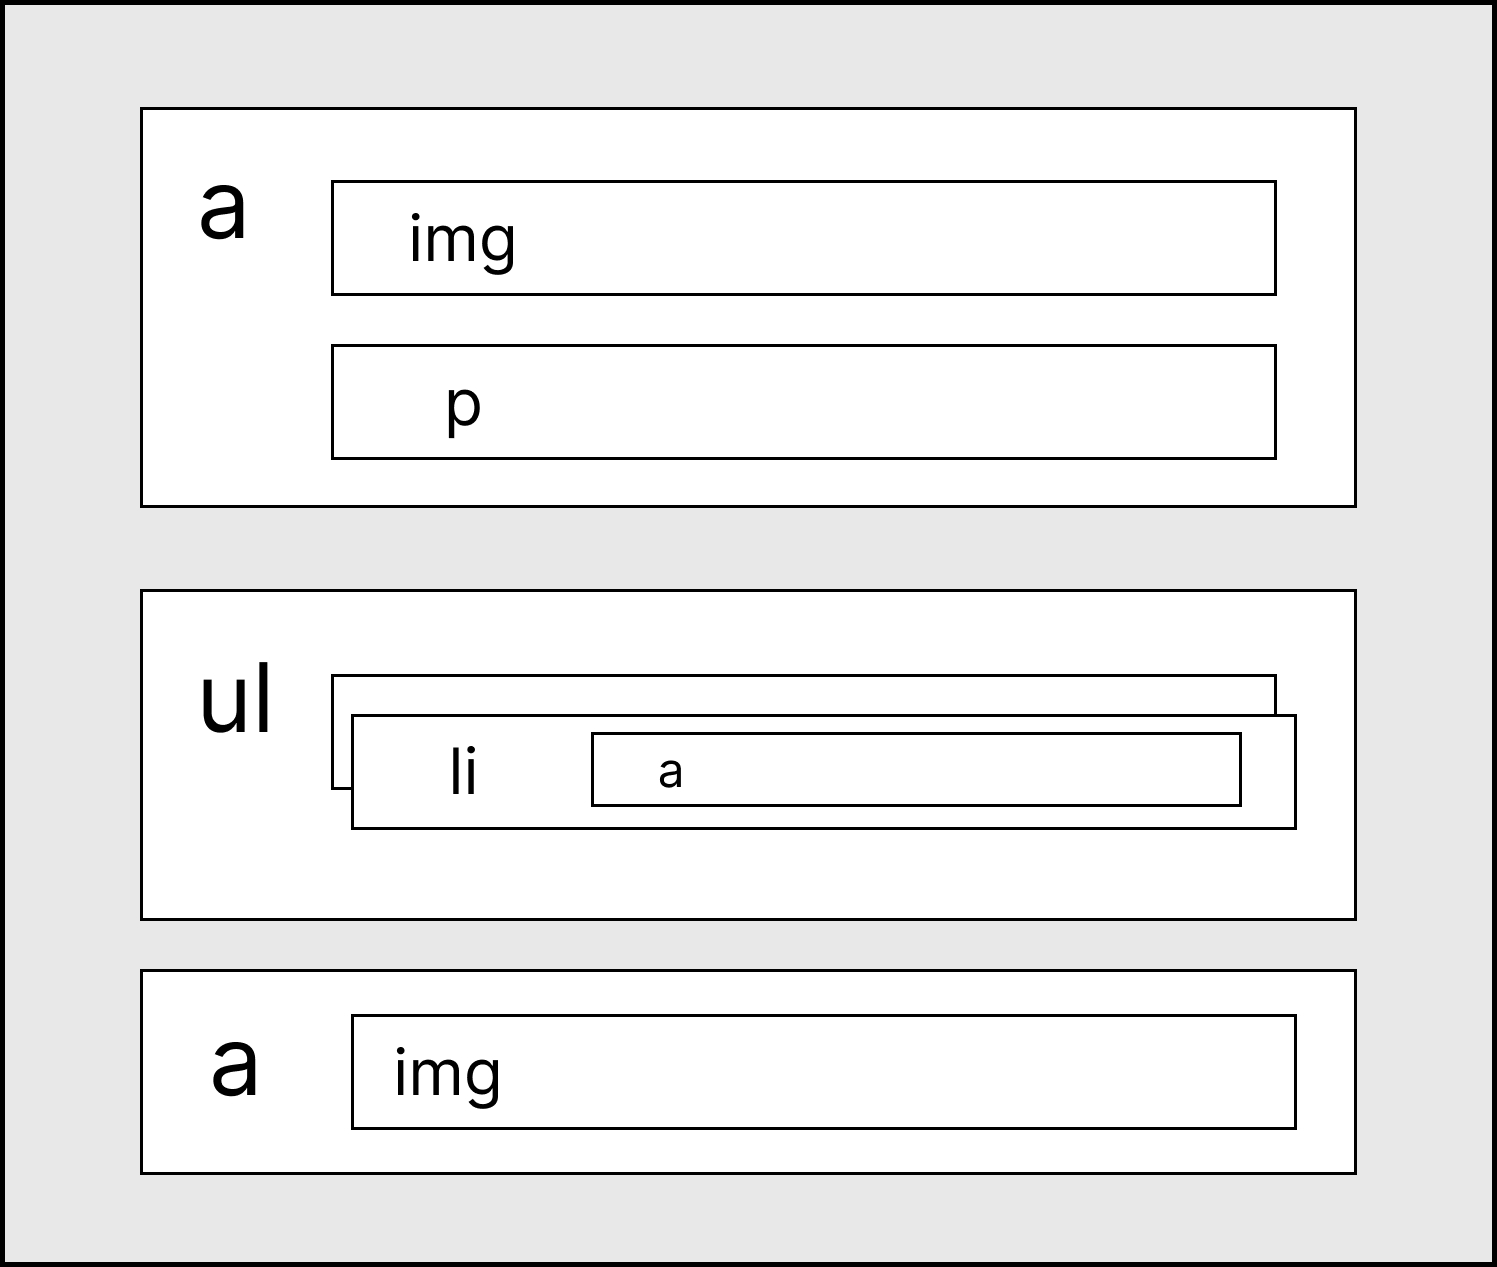
\includegraphics[width=0.6\textwidth]{HTML/Etiq-nav.jpg}
		\caption{Mapa de etiquetas menú de navegación}
	\end{figure}
	
	En el mapa de etiquetas del menú de navegación se entra en más detalles, donde se puede ver que el logo junto al nombre de la empresa son un enlace que lleva a la página principal, la cual se acaba de mostrar. El resto son una lista, a la que se le eliminará el formato, de texto con un hiperenlace, a excepción del botón de \textit{login}, que es de nuevo una imagen.
	
	\begin{figure} [H]
		\centering
		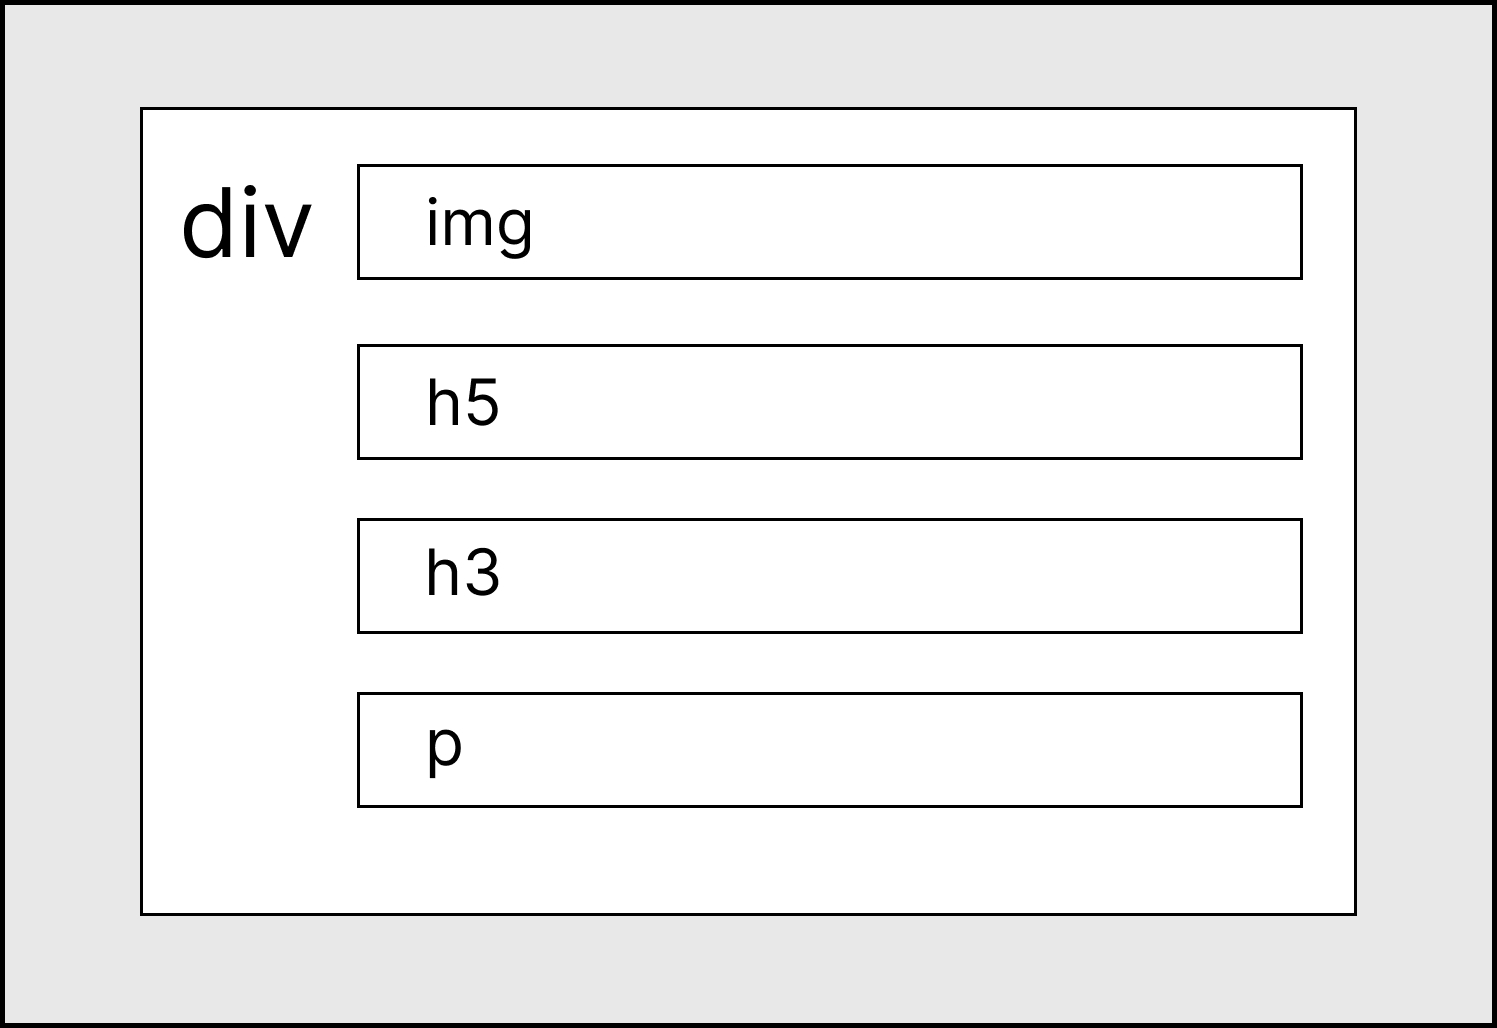
\includegraphics[width=0.6\textwidth]{HTML/Etiq-valoracion.jpg}
		\caption{Mapa de etiquetas valoración}
	\end{figure}

	También se incluyen los elementos de una caja de valoración, pues es relevante cómo se construye. Se ha decidido utilizar un \textbf{div} para englobar todos los elementos y poder replicarla con facilidad manteniendo sus propiedades. De esta forma, está compuesta por una imagen, correspondiente a la foto de perfil del usuario, junto a su nombre y puntuación en el encabezado \textbf{h5}. A continuación aparece el título de la reseña y su descripción.

	\begin{Huge}
		\textcolor{red}{Doc Descubre + Mapa etiquetas}
	\end{Huge}

	\begin{figure} [H]
		\centering
		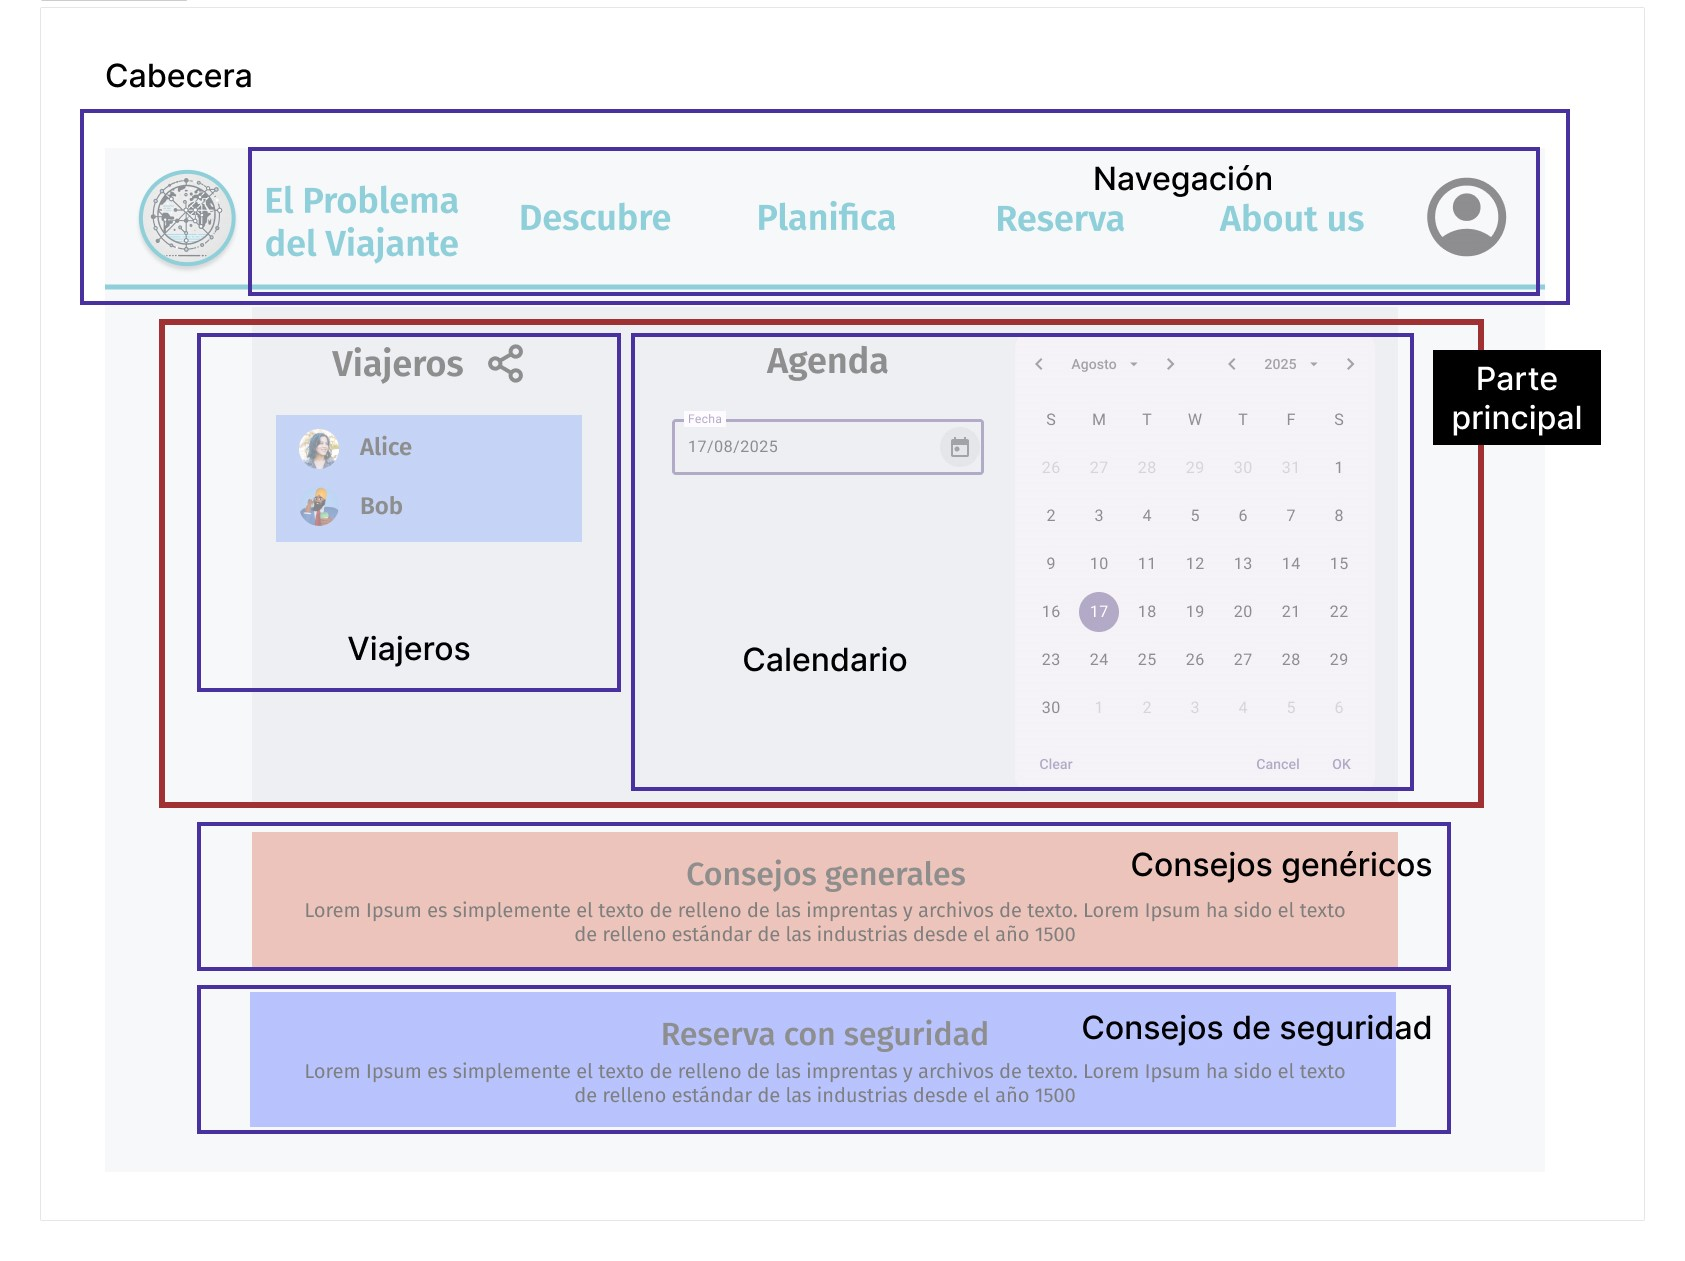
\includegraphics[width=\textwidth]{HTML/Doc-planifica.jpg}
		\caption{Elementos Planifica}
	\end{figure}

	En la parte principal de la planificación, se puede ver una lista de personas con los que se comparte el viaje y la organización de las actividades del mismo. Junto a él, el calendario donde propiamente se gestiona la planificación. Se entrará en más detalles en el mapa de etiquetas de cada uno. En la zona inferior, se muestran diferentes consejos que pueden ayudar a la gestión del viaje.
	
	\begin{figure} [H]
		\centering
		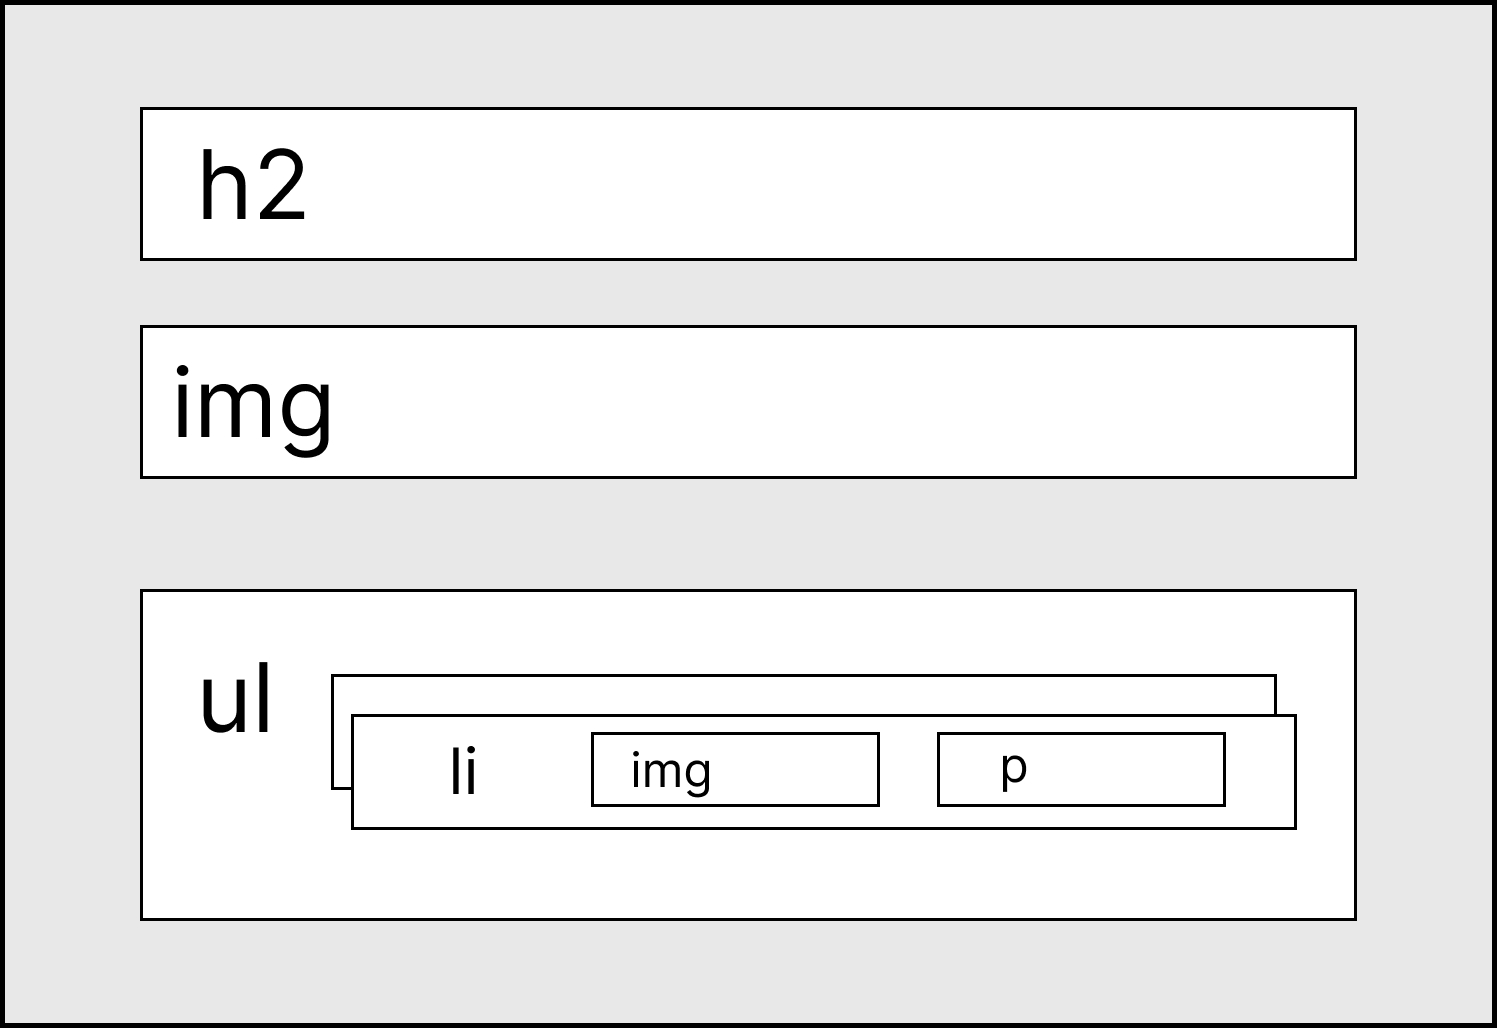
\includegraphics[width=0.6\textwidth]{HTML/Etiq-viajeros.jpg}
		\caption{Mapa de etiquetas viajeros}
	\end{figure}

	En la zona de los viajeros, se muestra el título junto a una imagen, que es un botón para compartir la planificación con otras personas, y así poder añadirlas al viaje fácilmente. A continuación, se muestra una lista de usuarios, que son precisamente los que ya se han incluido en la gestión del viaje y, de forma similar a como aparecía en la caja de valoraciones, aparece su foto de perfil y su nombre.

	\begin{figure} [H]
		\centering
		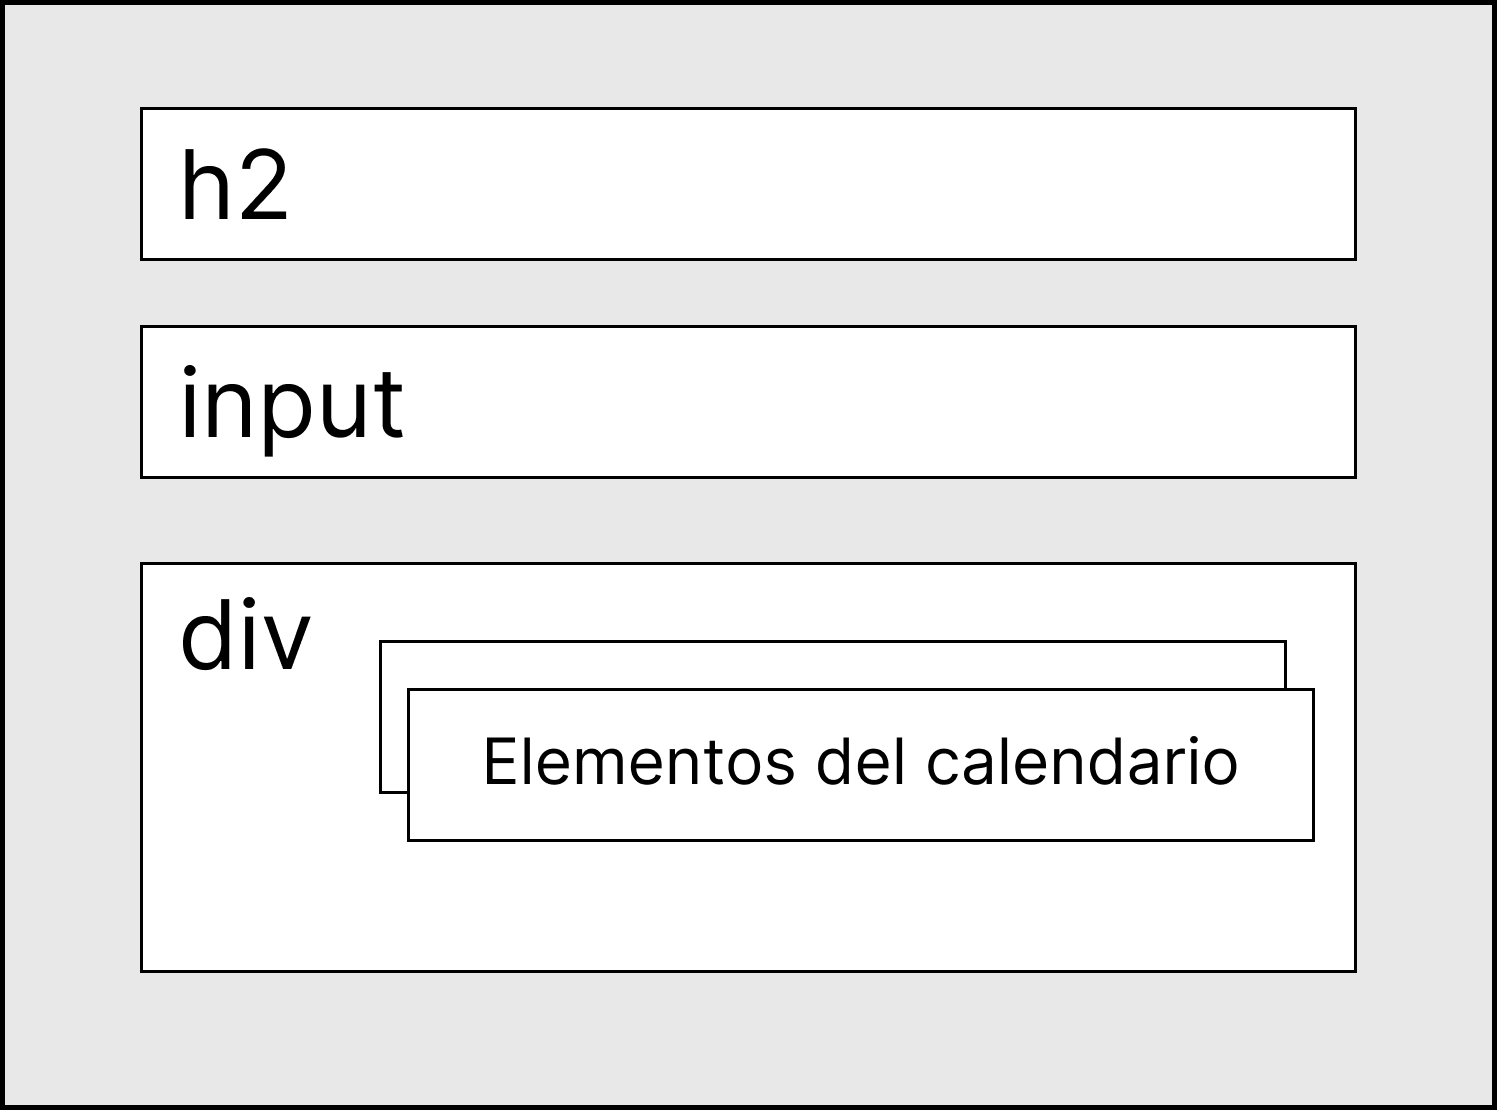
\includegraphics[width=0.6\textwidth]{HTML/Etiq-calendario.jpg}
		\caption{Mapa de etiquetas calendario}
	\end{figure}

	La caja del calendario es la más importante de todas, pues es la que permitirá realmente la gestión del viaje. En el mapa de etiquetas aparece el título junto a un \textbf{input}, desde el cual se puede introducir una fecha, asociada a la posición del calendario. El calendario en sí no está programado con HTML, ya que será necesario utilizar JavaScript para dotarlo de la responsividad que necesita.

	\begin{Huge}
		\textcolor{red}{Doc Reserva + Mapa etiquetas}
	\end{Huge}

	\begin{figure} [H]
		\centering
		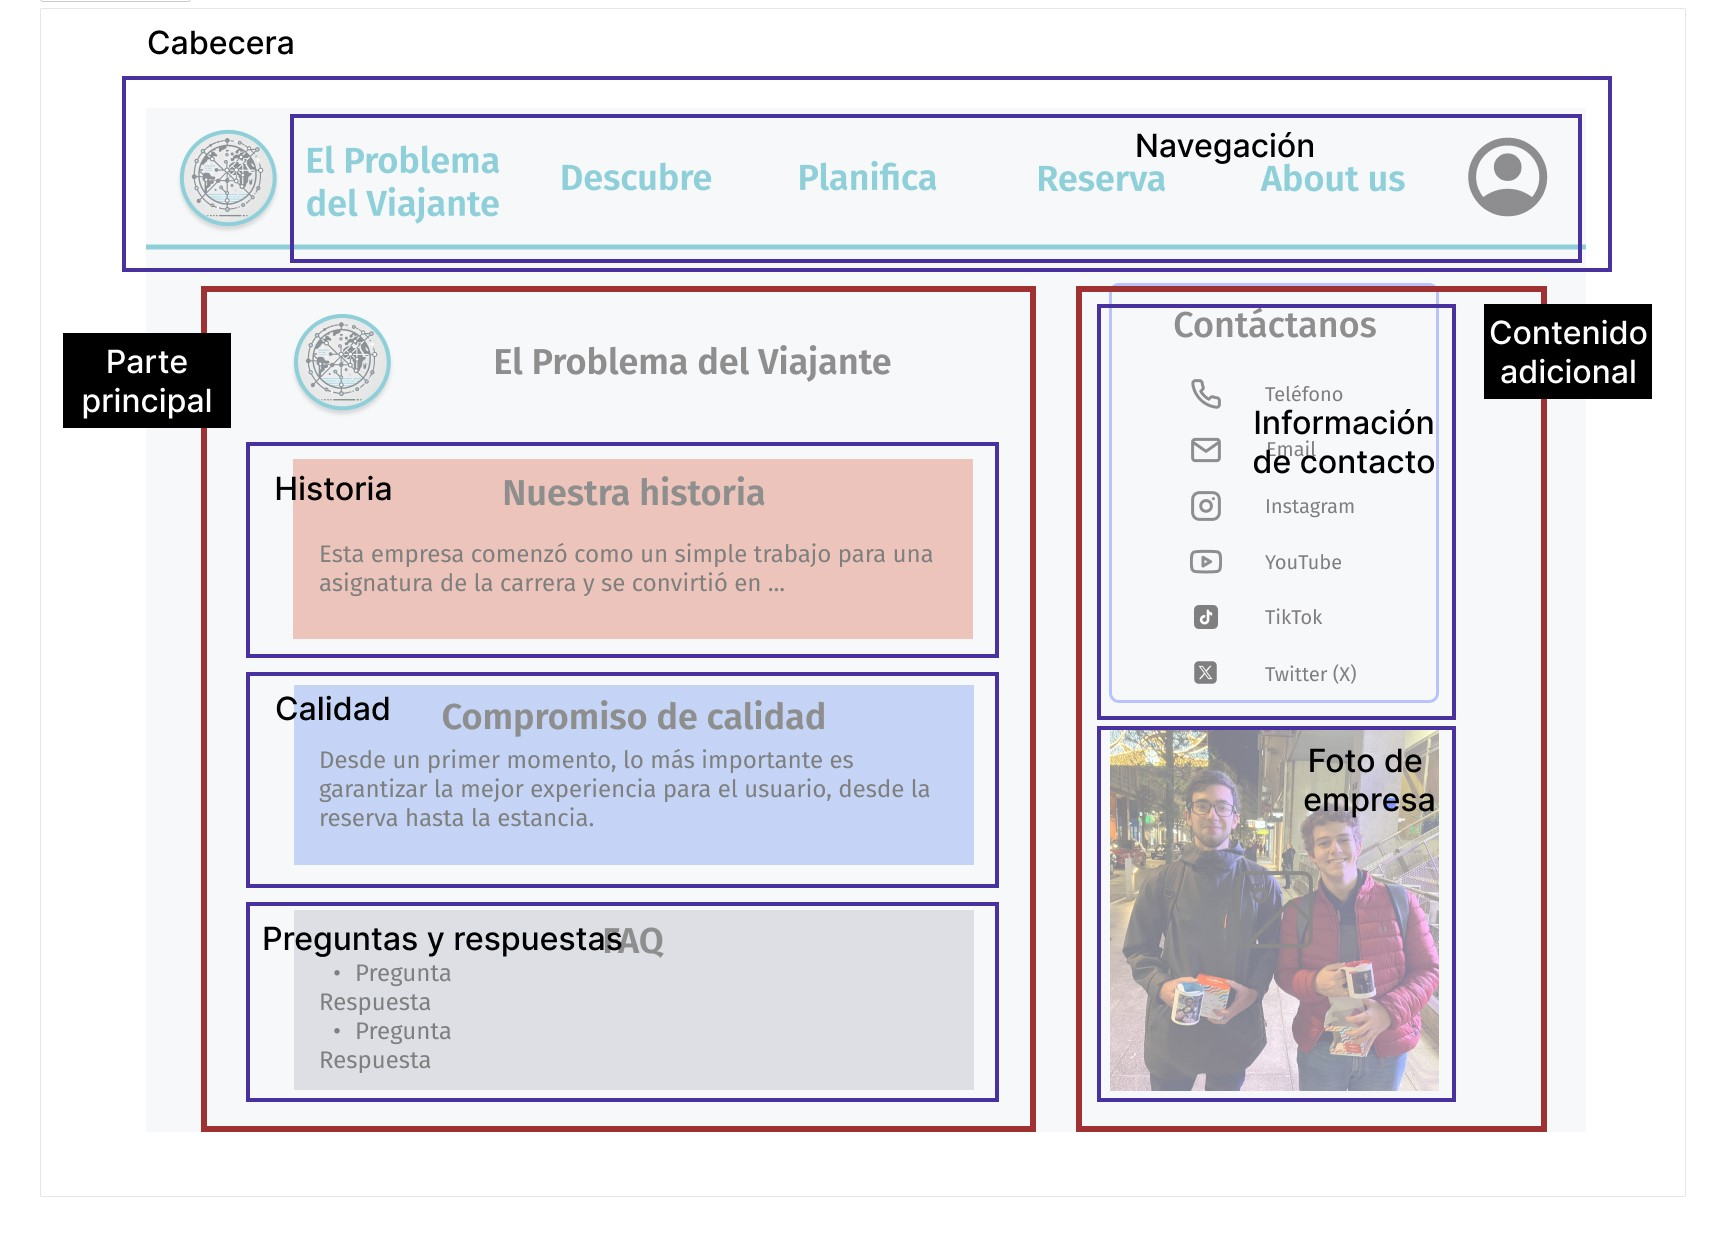
\includegraphics[width=0.8\textwidth]{HTML/Doc-about_us.jpg}
		\caption{Elementos About us}
	\end{figure}

	Esta es la página más simple de las cinco principales, ya que tiene una zona principal con los diferentes apartados que hablan sobre la empresa, sus características y preguntas frecuentes. Por otro lado, en el lateral hay una lista con diferentes formas de contacto con la empresa y todas sus redes sociales, desde las que se podría acceder a más información sobre ella, y ver más imágenes sobre posibles destinos de vacaciones.
	
	
	La mayoría de las otras páginas de la web son muy semejantes a las mostradas (por ejemplo, en las que tienen un menú de navegación secundario, las diferencias entre sí son ínfimas), y otras como la pestaña de Política de privacidad o Términos y condiciones solamente tienen contenido de texto a una columna, por lo que no aporta información mostrar su mapa de etiquetas.
	
	
	
	
	
	
	% ----------------------------------------------------------------------------
	% ----------------------------------------------------------------------------
	
	\chapter{Documentación CSS}
	
	\section{Flexible Grids}
	Este es el mecanismo convencional para conseguir la responsividad, mediante el uso \textit{float} y con anchos relativos. Se ha utilizado en la página About us de la siguiente manera: hay una zona principal en la que se comenta la historia de la empresa y los estándares de calidad, y un apartado secundario con información de contacto y redes sociales.
	
	El reparto del espacio no es equitativo, sino que se le da mayor importancia a los elementos principales. Además, se limita el ancho máximo de cada columna con el objetivo de que no se expandan horizontalmente demasiado en pantallas grandes. Se añaden dos puntos de ruptura, uno que reajusta los anchos de cada columna en pantallas de tamaño medio, y otro que eliminar el \textit{float} y convierte el diseño a una columna en pantallas pequeñas. A continuación se muestra un código simplificado del funcionamiento de \textit{flexible grids} y sus correspondientes capturas de pantalla.
	
	\begin{lstlisting}[]
.column1 {
	width: 65%;
	max-width: 800px;
	float: left;
}
.column2 {
	width: 25%;
	max-width: 300px;
	float: right;
}

@media screen and (max-width: 900px) {
	.column1 {
		width: 90%;
		float: none;
	}
	.column2 {
		width: 90%;
		float: none;
	}
}
	\end{lstlisting}

	\begin{figure} [H]
		\centering
		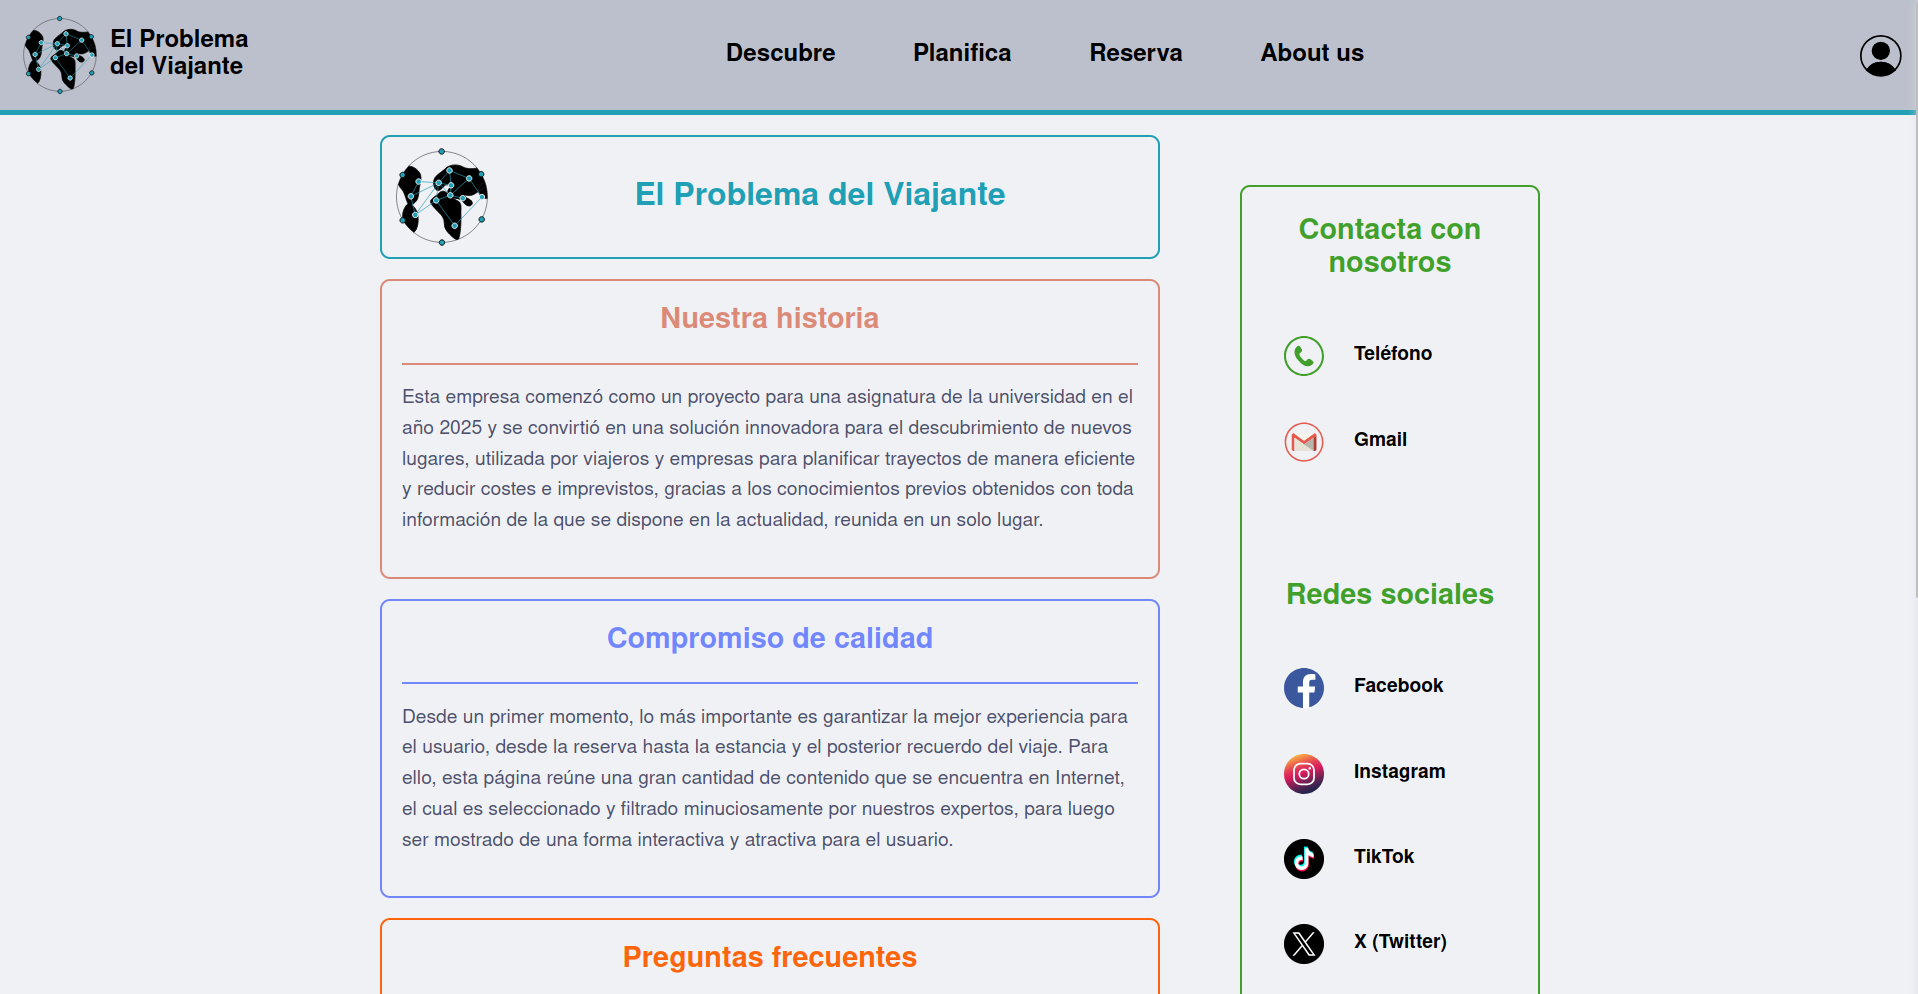
\includegraphics[width=\textwidth]{CSS/3-1 1920.png}
		\caption{Página About us - Ancho 1920px}
	\end{figure}

	La figura anterior muestra cómo se vería en un ordenador actual. El contenido aparece centrado, y la información de contacto y redes sociales hacia el lateral.
	
	\begin{figure} [H]
		\centering
		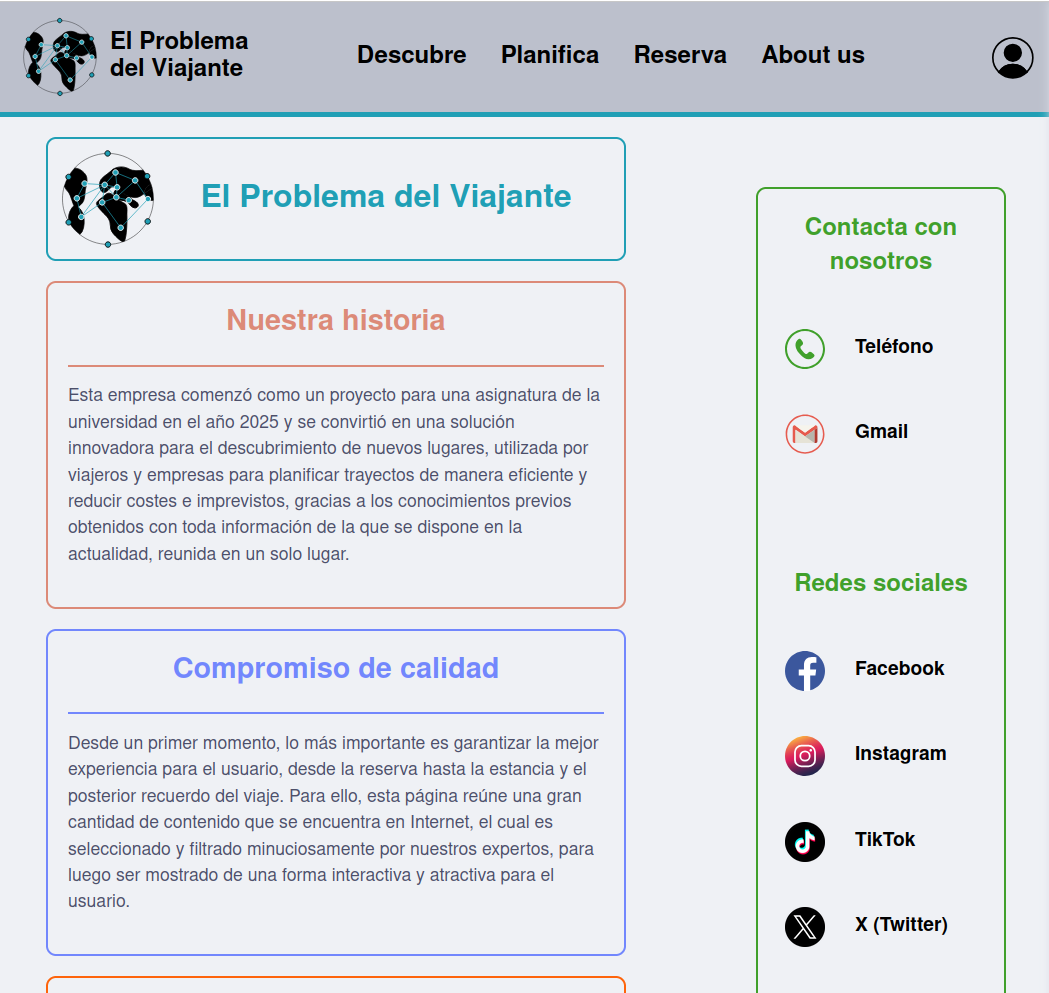
\includegraphics[height=0.4\textheight]{CSS/3-3 1024.png}
		\caption{Página About us - Ancho 1024px}
	\end{figure}

	Así se mostraría el contenido en un ordenador antiguo. La letra de los párrafos es ligeramente más pequeña, y cada columna es un poco menos ancha, para ajustarse a una pantalla más cuadrada.

	\begin{figure} [H]
		\centering
		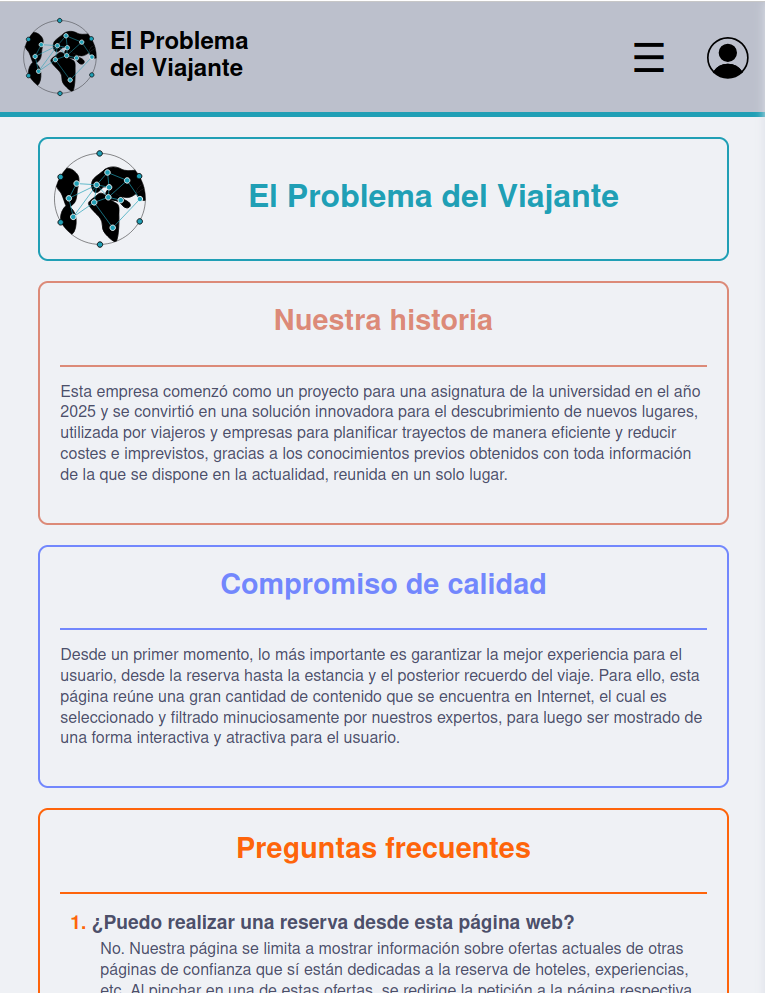
\includegraphics[height=0.4\textheight]{CSS/3-5 768.png}
		\caption{Página About us - Ancho 768px}
	\end{figure}
	\begin{figure} [H]
		\centering
		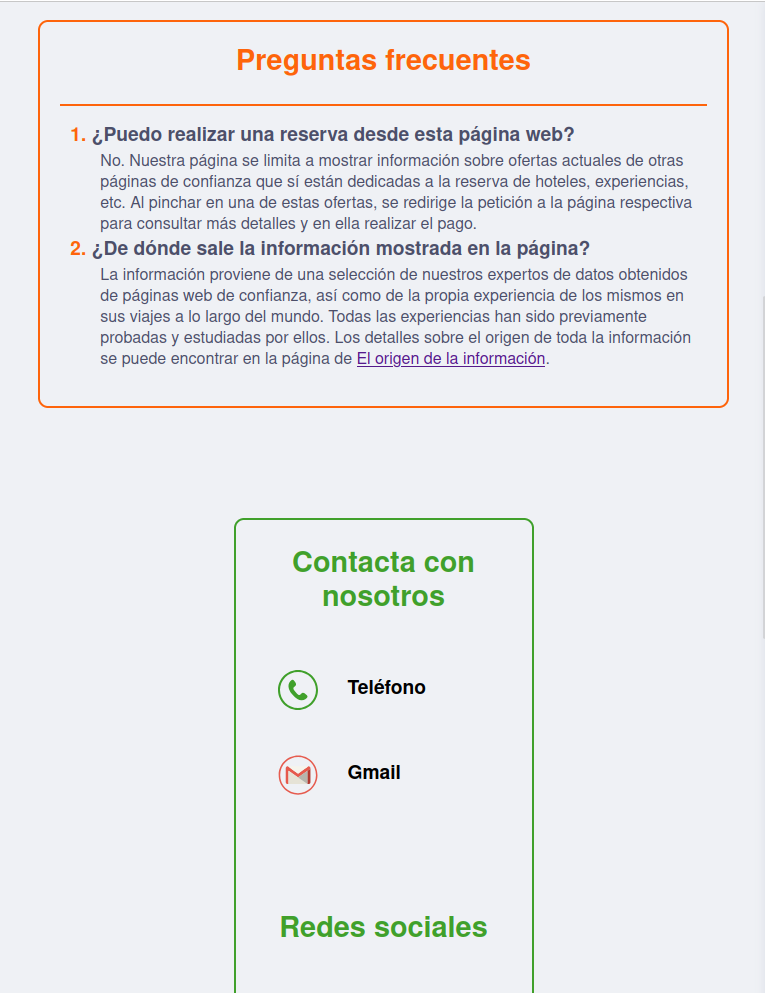
\includegraphics[height=0.4\textheight]{CSS/3-6 768.png}
		\caption{Página About us - Ancho 768px}
	\end{figure}

	De esta forma se muestra en un móvil, eliminando el diseño anterior y pasando a una columna. La sección de contacto y redes sociales ahora se mostraría más abajo, pero centrada. También se ajusta la letra y el interlineado consecuentemente.
	
	\begin{figure} [H]
		\centering
		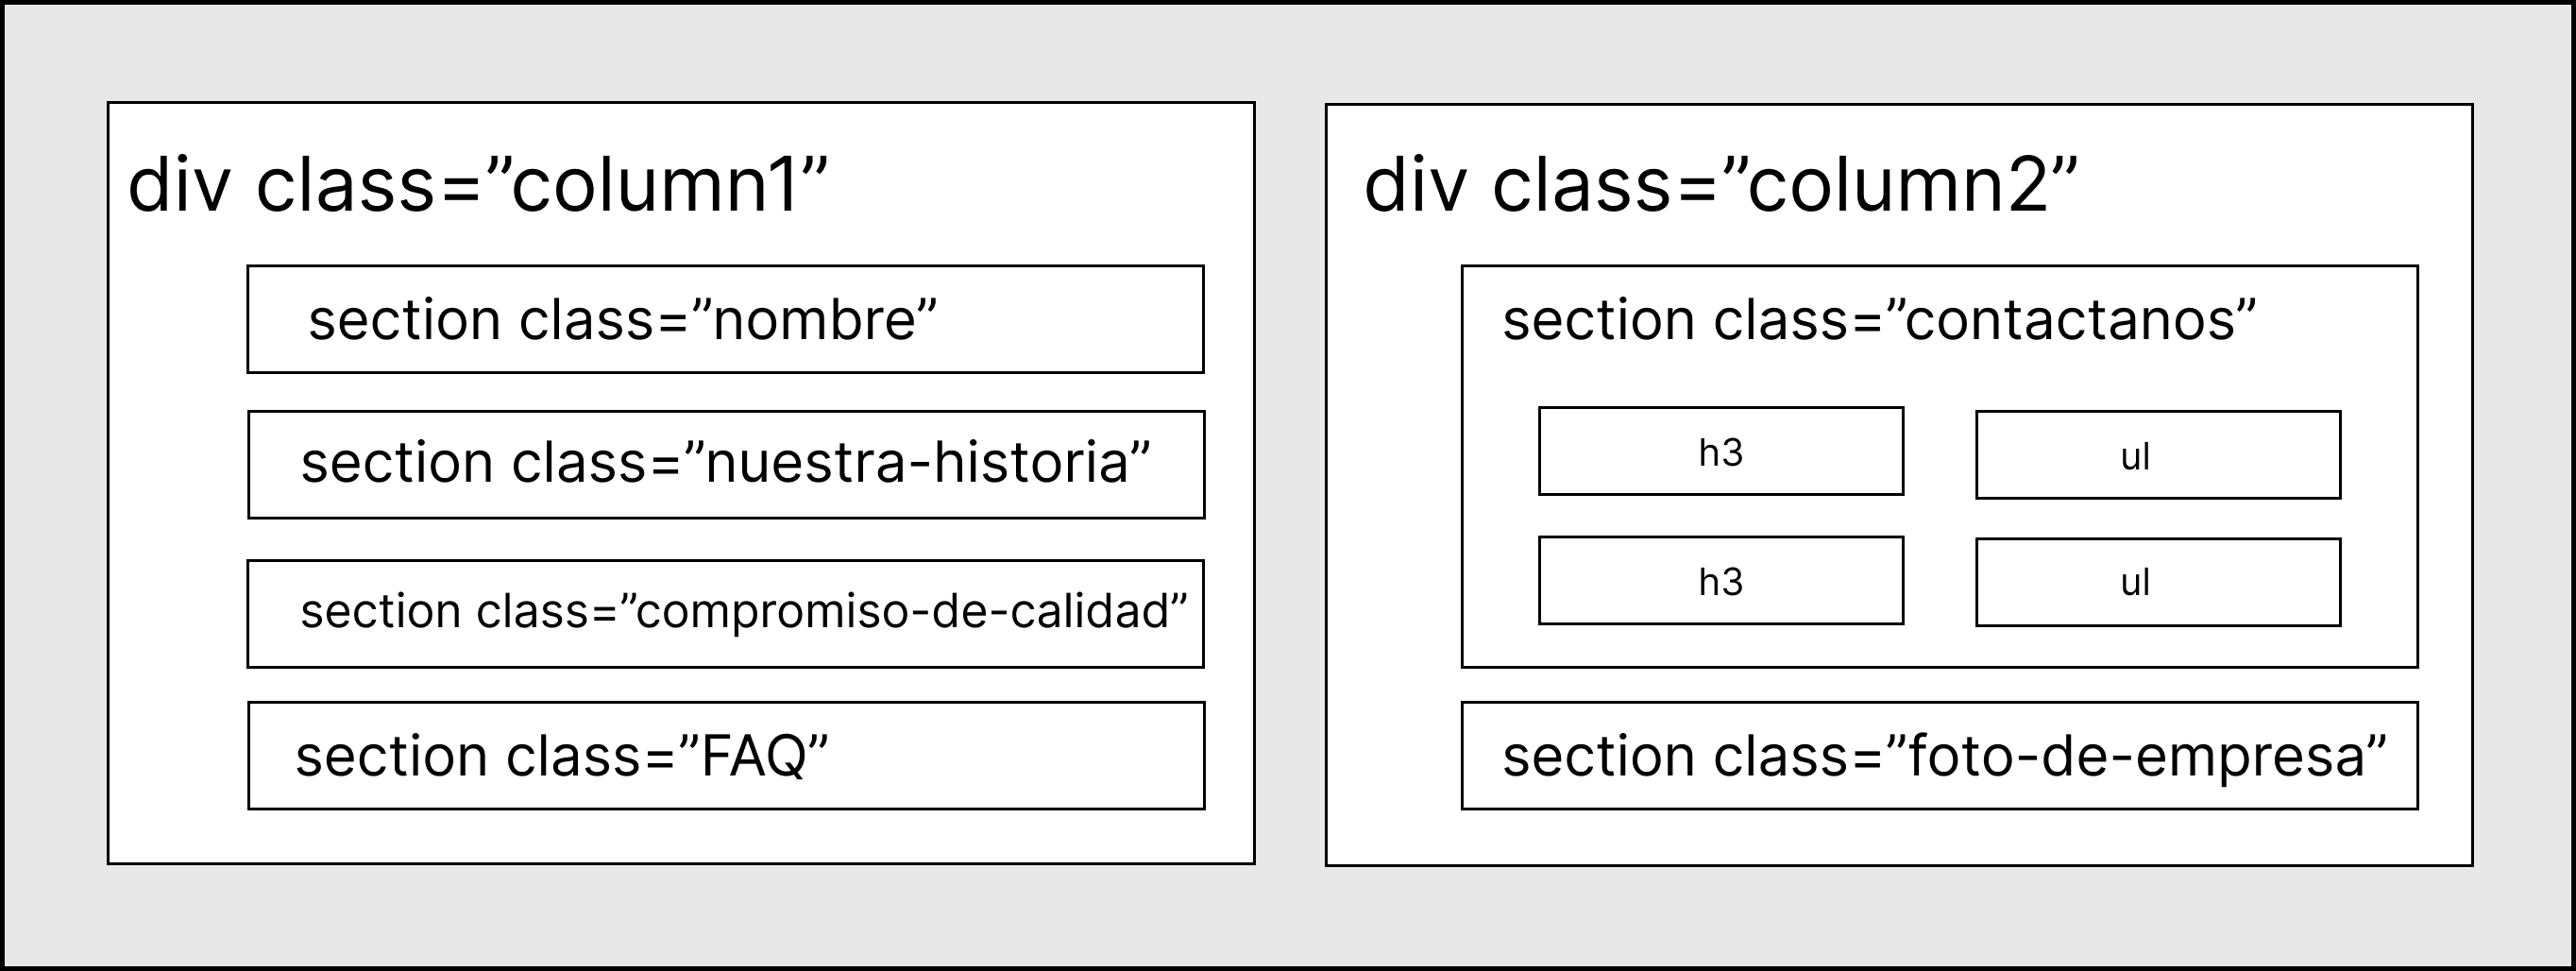
\includegraphics[width=0.8\textwidth]{CSS/CSS About us.jpg}
		\caption{Esquema About us}
	\end{figure}

	Se muestra en la imagen el esquema que sigue la página, que es bastante sencillo como se ha comentado. Tiene dos columnas, sobre las que se aplica el efecto, la primera está dividida en secciones, y están compuestas todas ellas por un encabezado y párrafos. La segunda columna tiene la sección de contacto, con dos listas, y la foto de empresa.

	
	\section{CSS Multicol}
	
	\begin{Huge}
		\textcolor{red}{Aquí va Descubre}
	\end{Huge}
	
	\section{Flex Container}
	
	\begin{Huge}
		\textcolor{red}{Aquí va Reserva}
	\end{Huge}

	\section{CSS Grid}
	El mecanismo \textit{CSS Grid} permite ajustar con precisión elementos en dos dimensiones, alineando con facilidad tanto las filas como las columnas. Ha resultado muy útil su uso en la página Planifica, ya que hay muchos elementos dispuestos de forma horizontal, y que van cambiando hacia un diseño más vertical según se reduce el ancho de la pantalla.
	
	De esta forma, se parte de un diseño en el que aparecen en la primera fila tanto los viajeros como el calendario de eventos. Un primer punto de ruptura acerca el contenido manteniendo su estructura, y el segundo punto de ruptura pasa a un diseño en el que se muestra todo en una columna, tal y como se ve en el código simplificado siguiente. 
	
	\begin{lstlisting}[]
.grid-container {
	display: grid;
	grid-template-columns: 1fr 1fr 1fr;
	grid-template-rows: auto;
	grid-template-areas:
	"travellers-title calendar-title  calendar-title"
	"travellers       calendar-events calendar"
	"advices          advices         advices"
	"security         security        security"
}

@media screen and (max-width: 1100px){
	.grid-container {
		grid-template-areas:
		"travellers-title"
		"travellers"
		"calendar-title"
		"calendar"
		"calendar-events"
		"advices"
		"security"
	}
}
	\end{lstlisting}
	
	\begin{figure} [H]
		\centering
		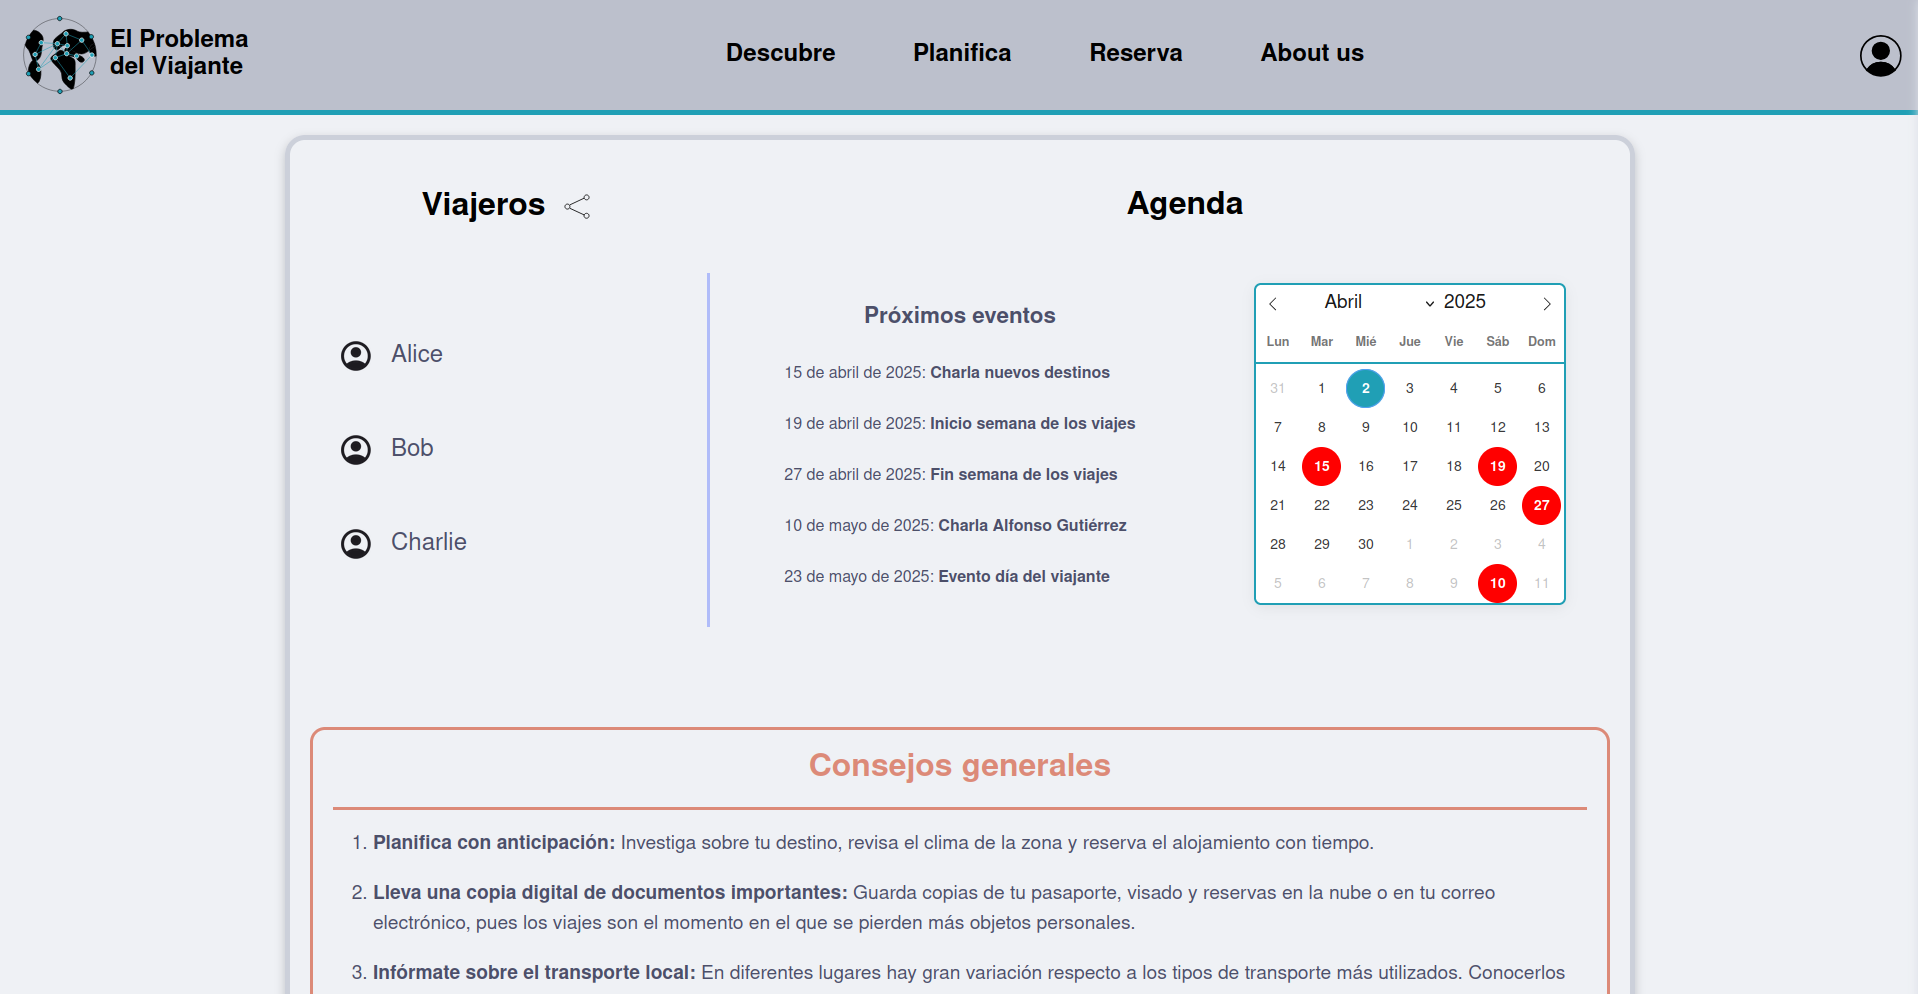
\includegraphics[width=\textwidth]{CSS/2-1 1920.png}
		\caption{Página Planifica - Ancho 1920px}
	\end{figure}

	En pantallas grandes, se muestra el \textit{grid} de esta forma. Como se ha comentado, aparece el calendario a la derecha, y los viajeros a la izquierda

	\begin{figure} [H]
		\centering
		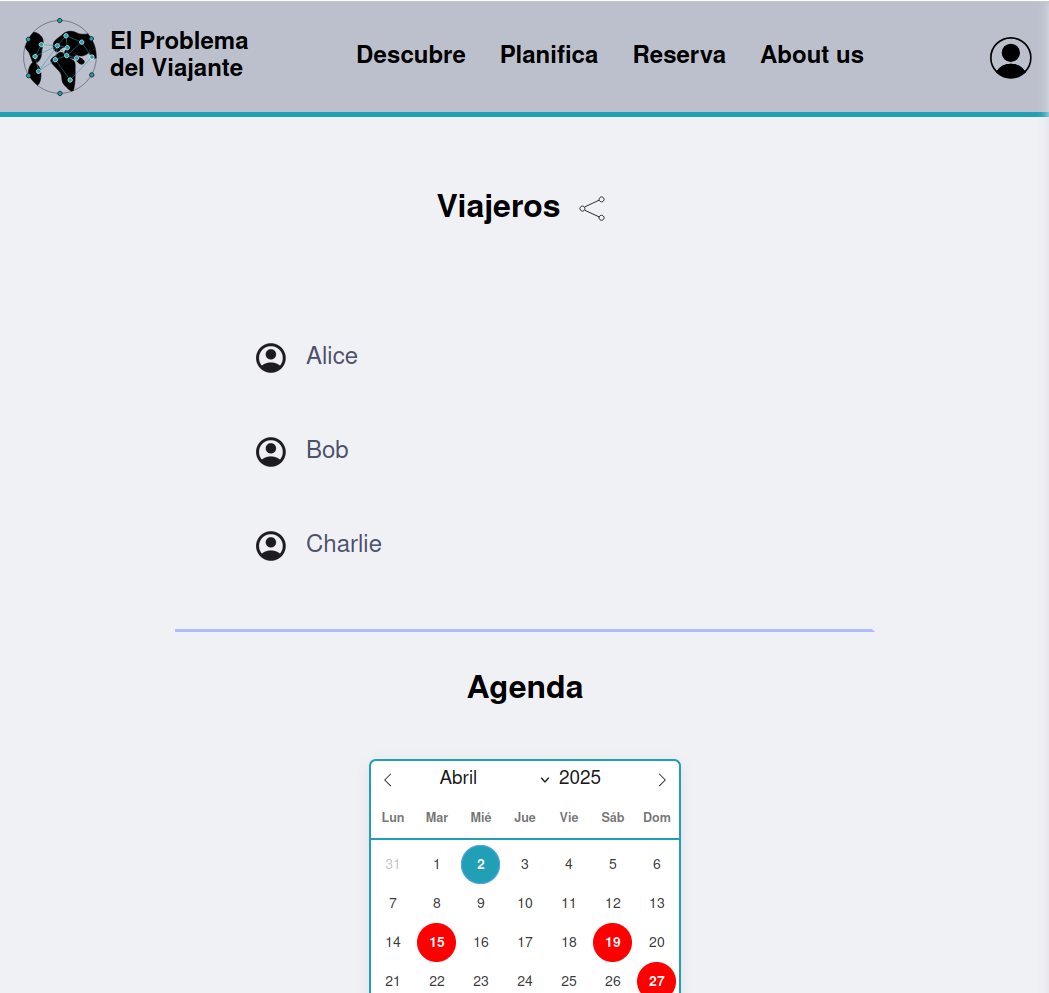
\includegraphics[height=0.4\textheight]{CSS/2-3 1024.png}
		\caption{Página Planifica - Ancho 1024px}
	\end{figure}
	\begin{figure} [H]
		\centering
		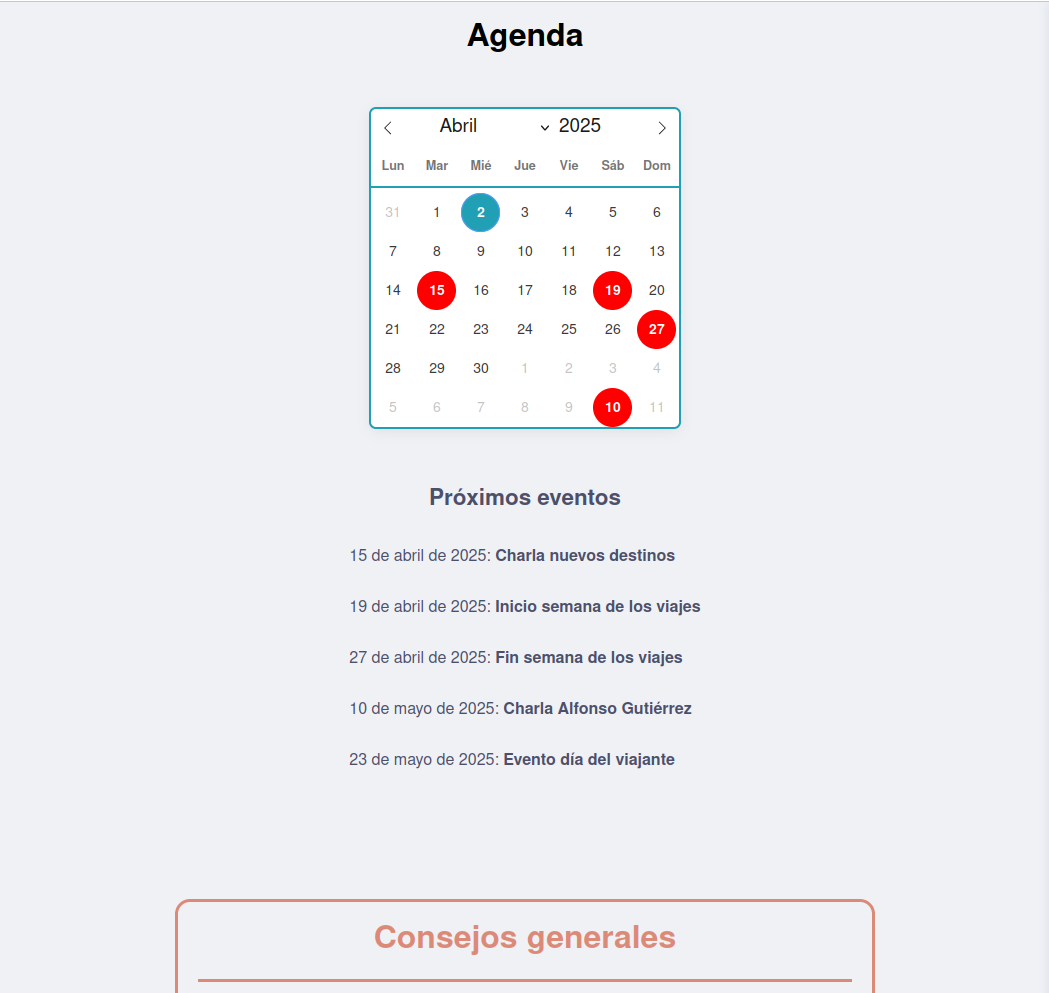
\includegraphics[height=0.4\textheight]{CSS/2-4 1024.png}
		\caption{Página Planifica - Ancho 1024px}
	\end{figure}

	En pantallas de tamaño medio, se pasa al diseño de una columna. La ventaja de usar \textit{CSS Grid} es que sería sencillo realizar cambios para que en un determinado lugar hubiese dos columnas, si así se quisiese.
	
	\begin{figure} [H]
		\centering
		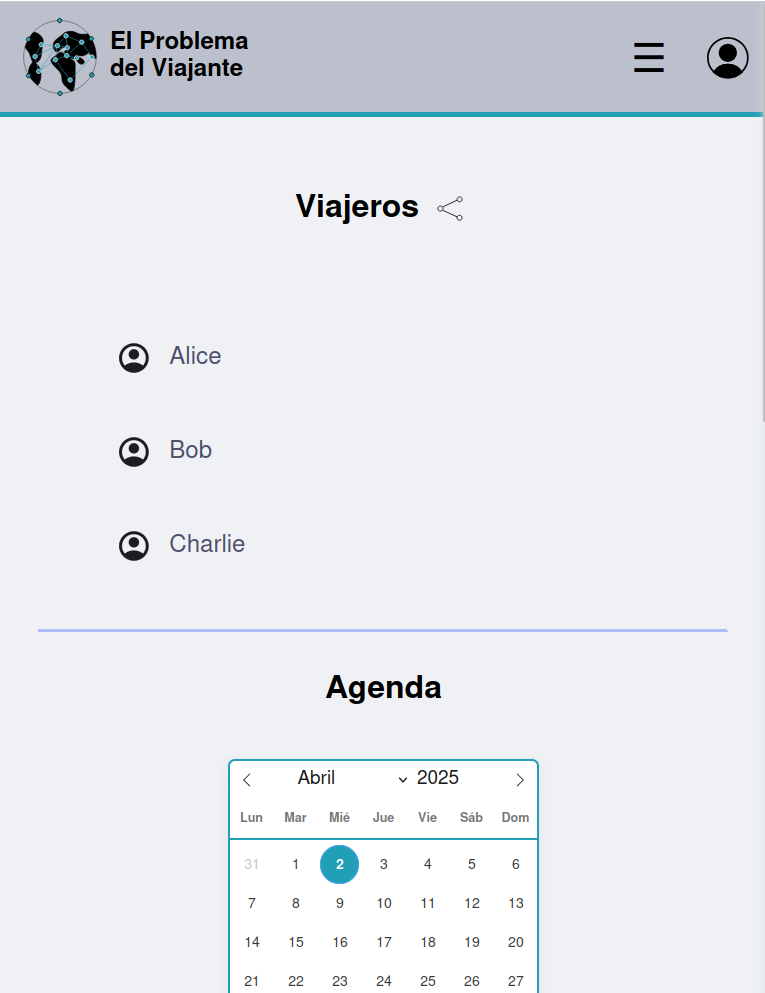
\includegraphics[height=0.4\textheight]{CSS/2-5 768.png}
		\caption{Página Planifica - Ancho 768px}
	\end{figure}
	\begin{figure} [H]
		\centering
		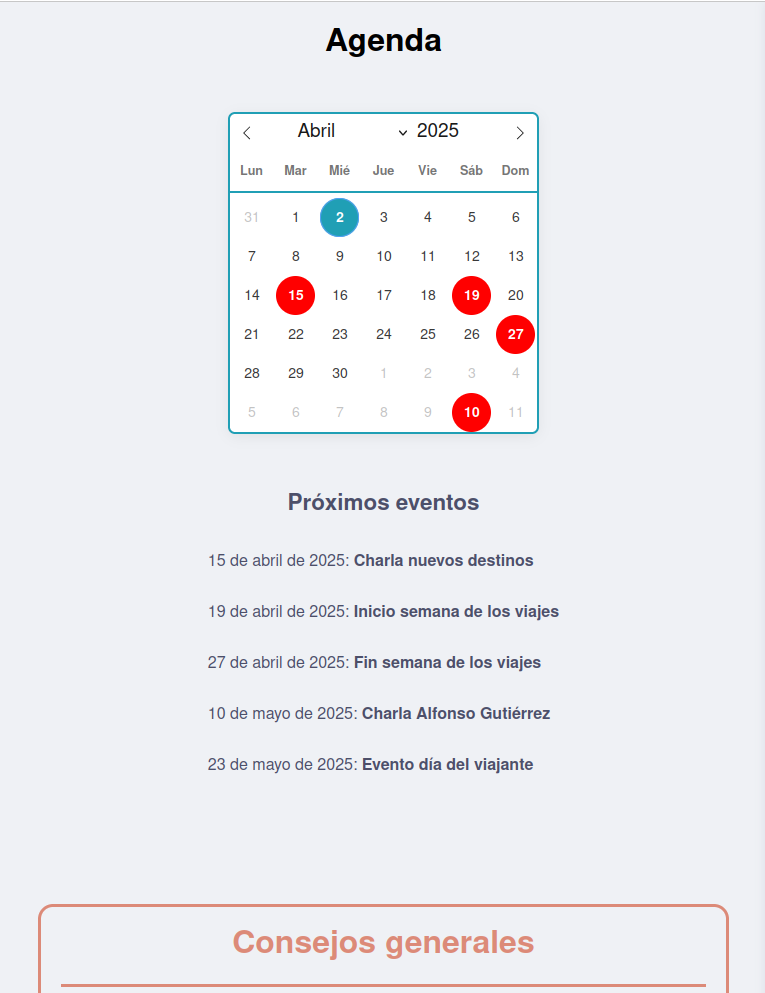
\includegraphics[height=0.4\textheight]{CSS/2-6 768.png}
		\caption{Página Planifica - Ancho 768px}
	\end{figure}

	Por último, el diseño se ajusta correctamente a pantallas pequeñas, de forma similar al anterior. 
	
	\begin{figure} [H]
		\centering
		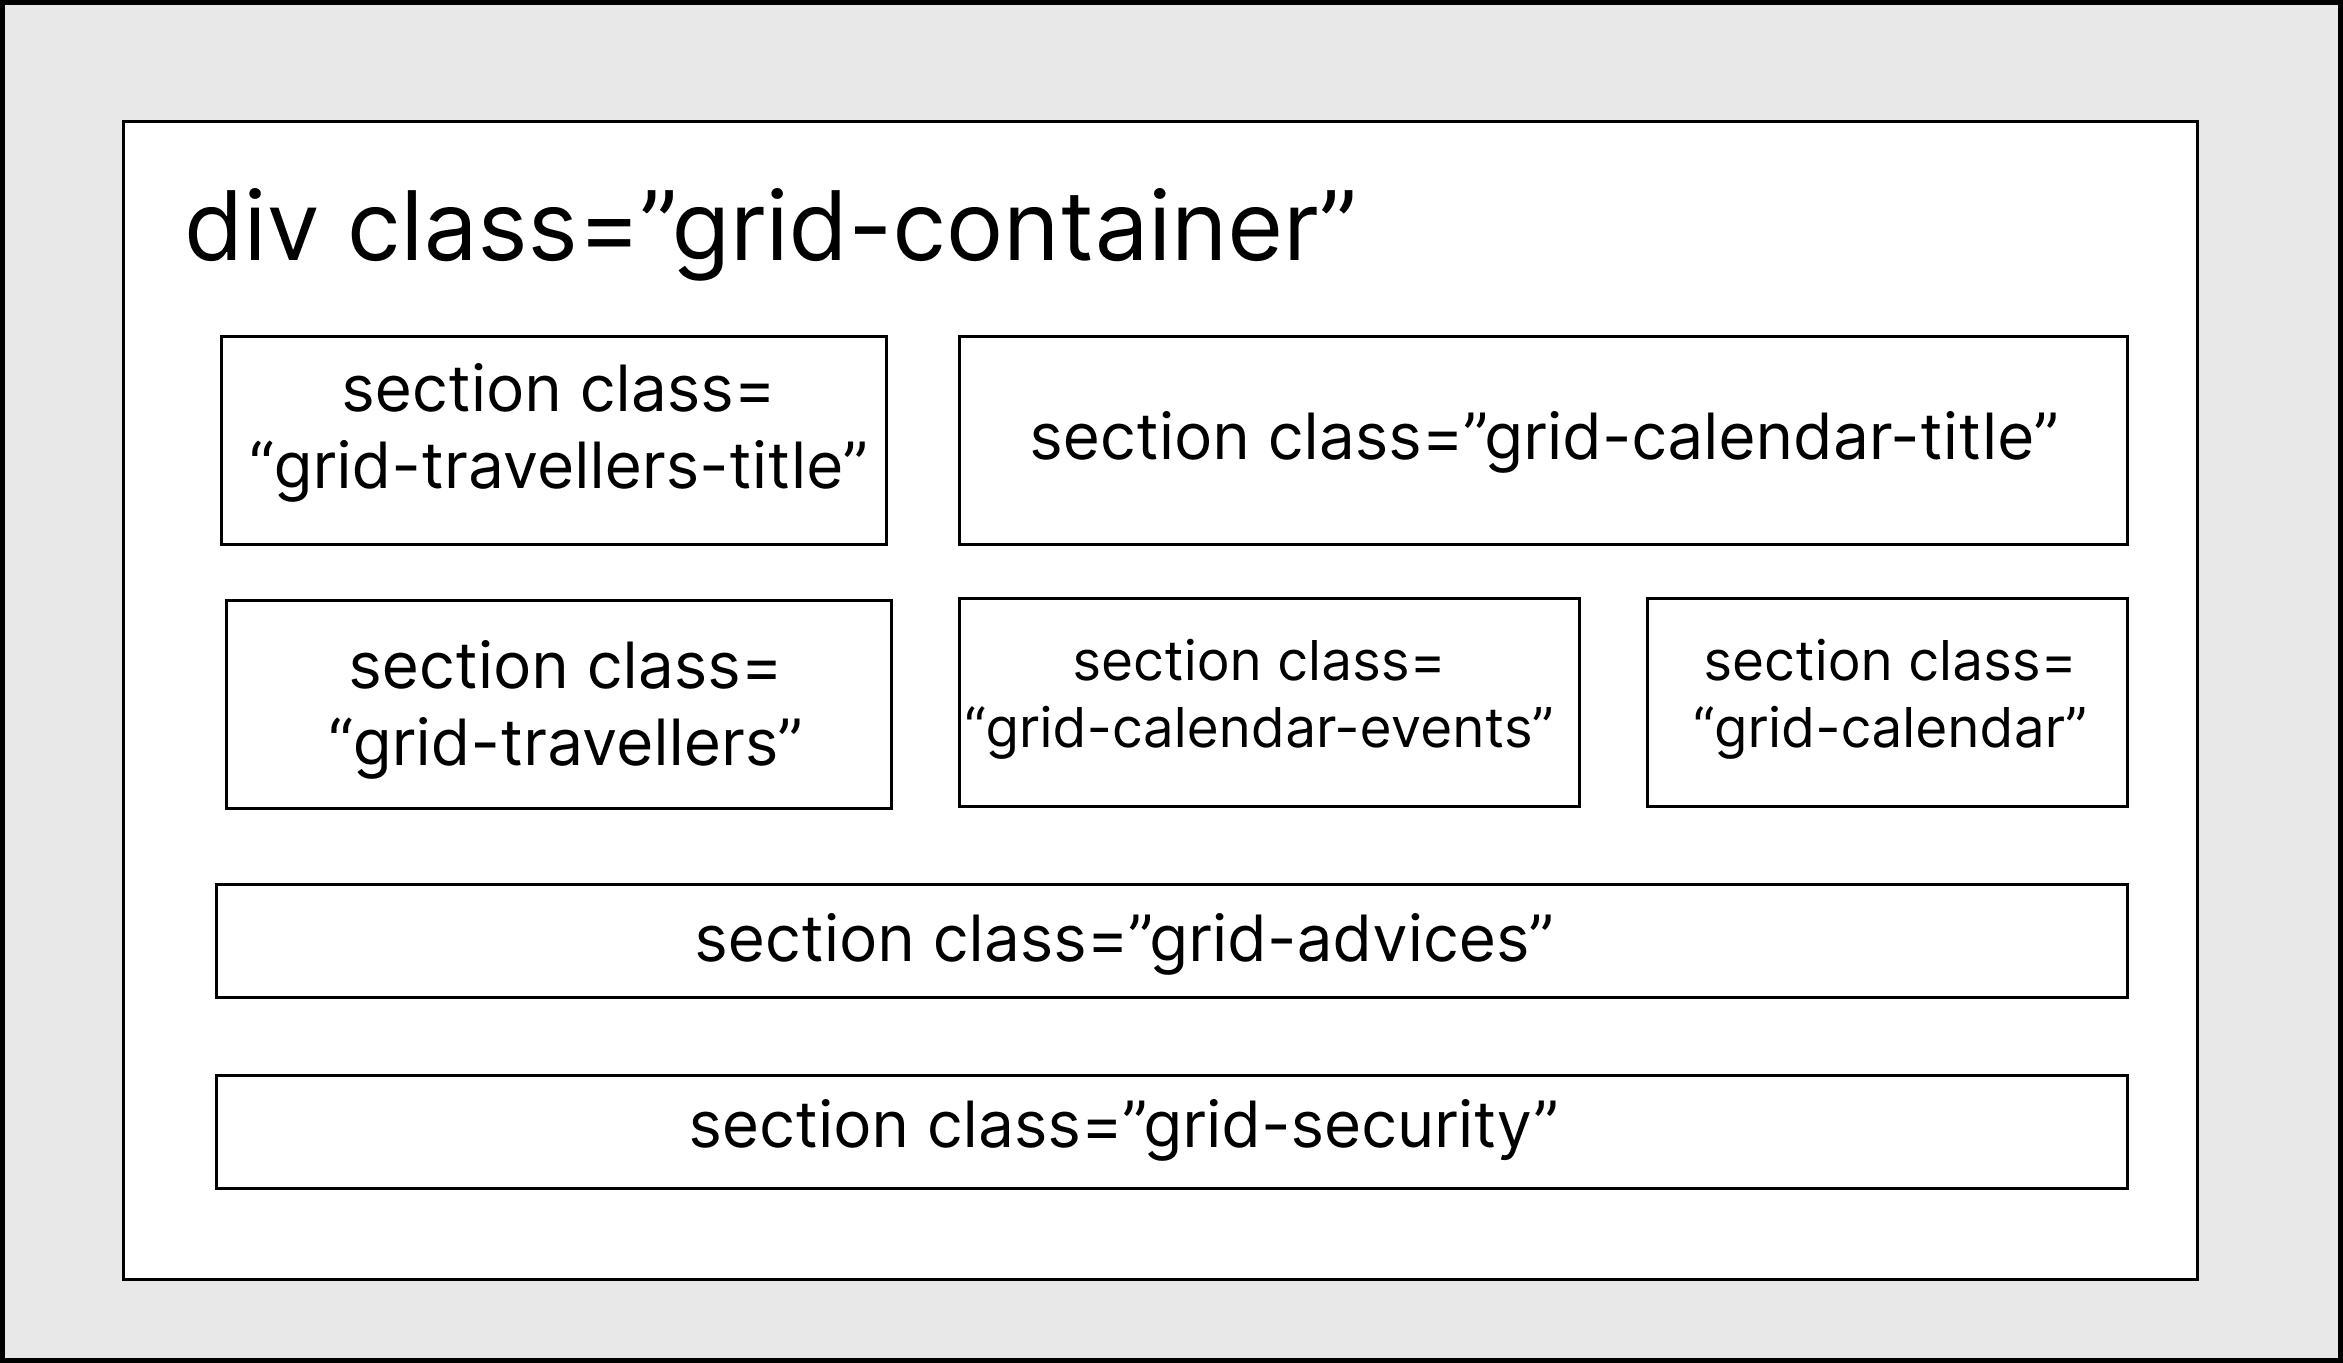
\includegraphics[width=0.8\textwidth]{CSS/CSS Planifica.jpg}
		\caption{Esquema Planifica}
	\end{figure}

	Para el esquema de esta página se ha decidido usar la misma disposición que aparece en el \textit{grid}, con el objetivo de facilitar la compresión de la posición de cada elemento en la página. Las clases de cada uno se corresponden precisamente con los nombres de la plantilla de \textit{grid} que se muestra en el código, junto a la palabra \textit{grid}, y que están asignados en el archivo CSS.

	
	\section{Bootstrap}
	\textit{Bootstrap} es una librería de reglas CSS que permite reducir significativamente la cantidad de código propio necesario para desarrollar la página, a cambio de utilizar ciertas características predeterminadas. También permite añadir más variabilidad a los diseños, y en este caso se ha realizado un cambio respecto al diseño inicial en la página principal, pues se ha incluido un carrusel de imágenes (más detalles en el \nameref{chap:anexo1}).
	
	\begin{figure} [H]
		\centering
		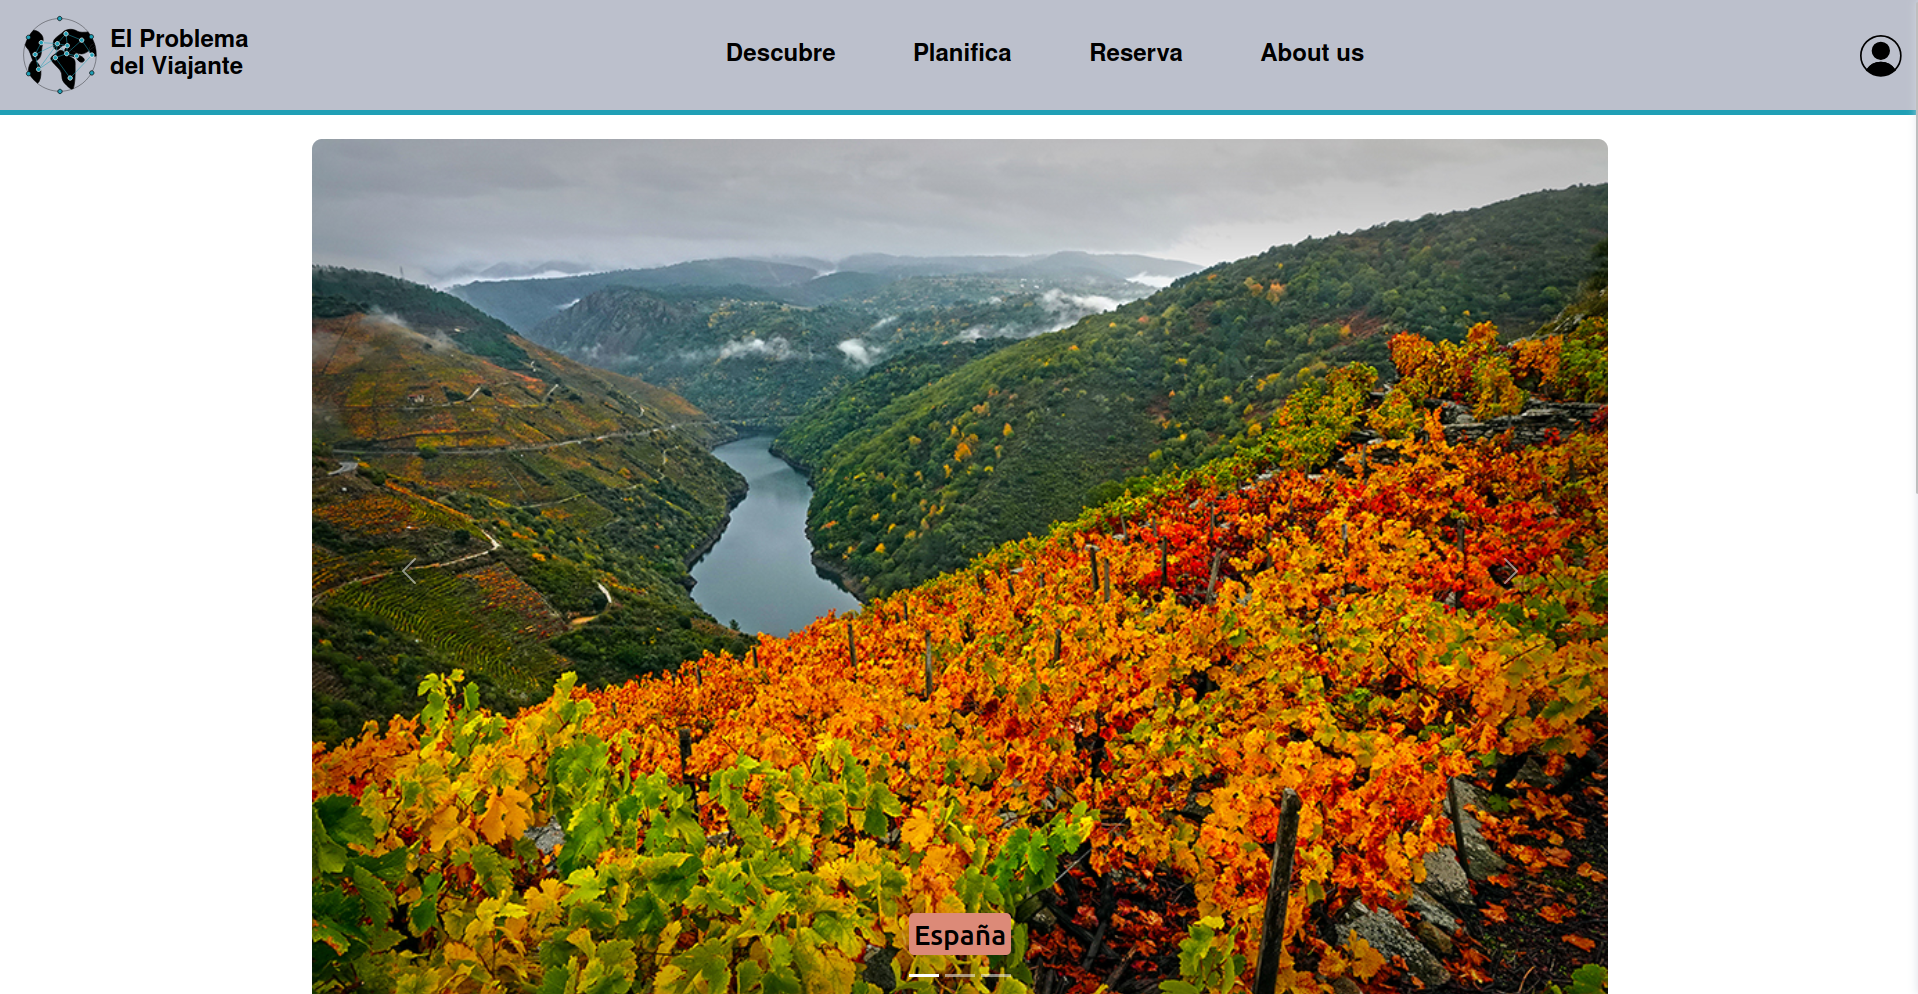
\includegraphics[width=\textwidth]{CSS/1-1 1920.png}
		\caption{Página principal - Ancho 1920px}
	\end{figure}
	\begin{figure} [H]
		\centering
		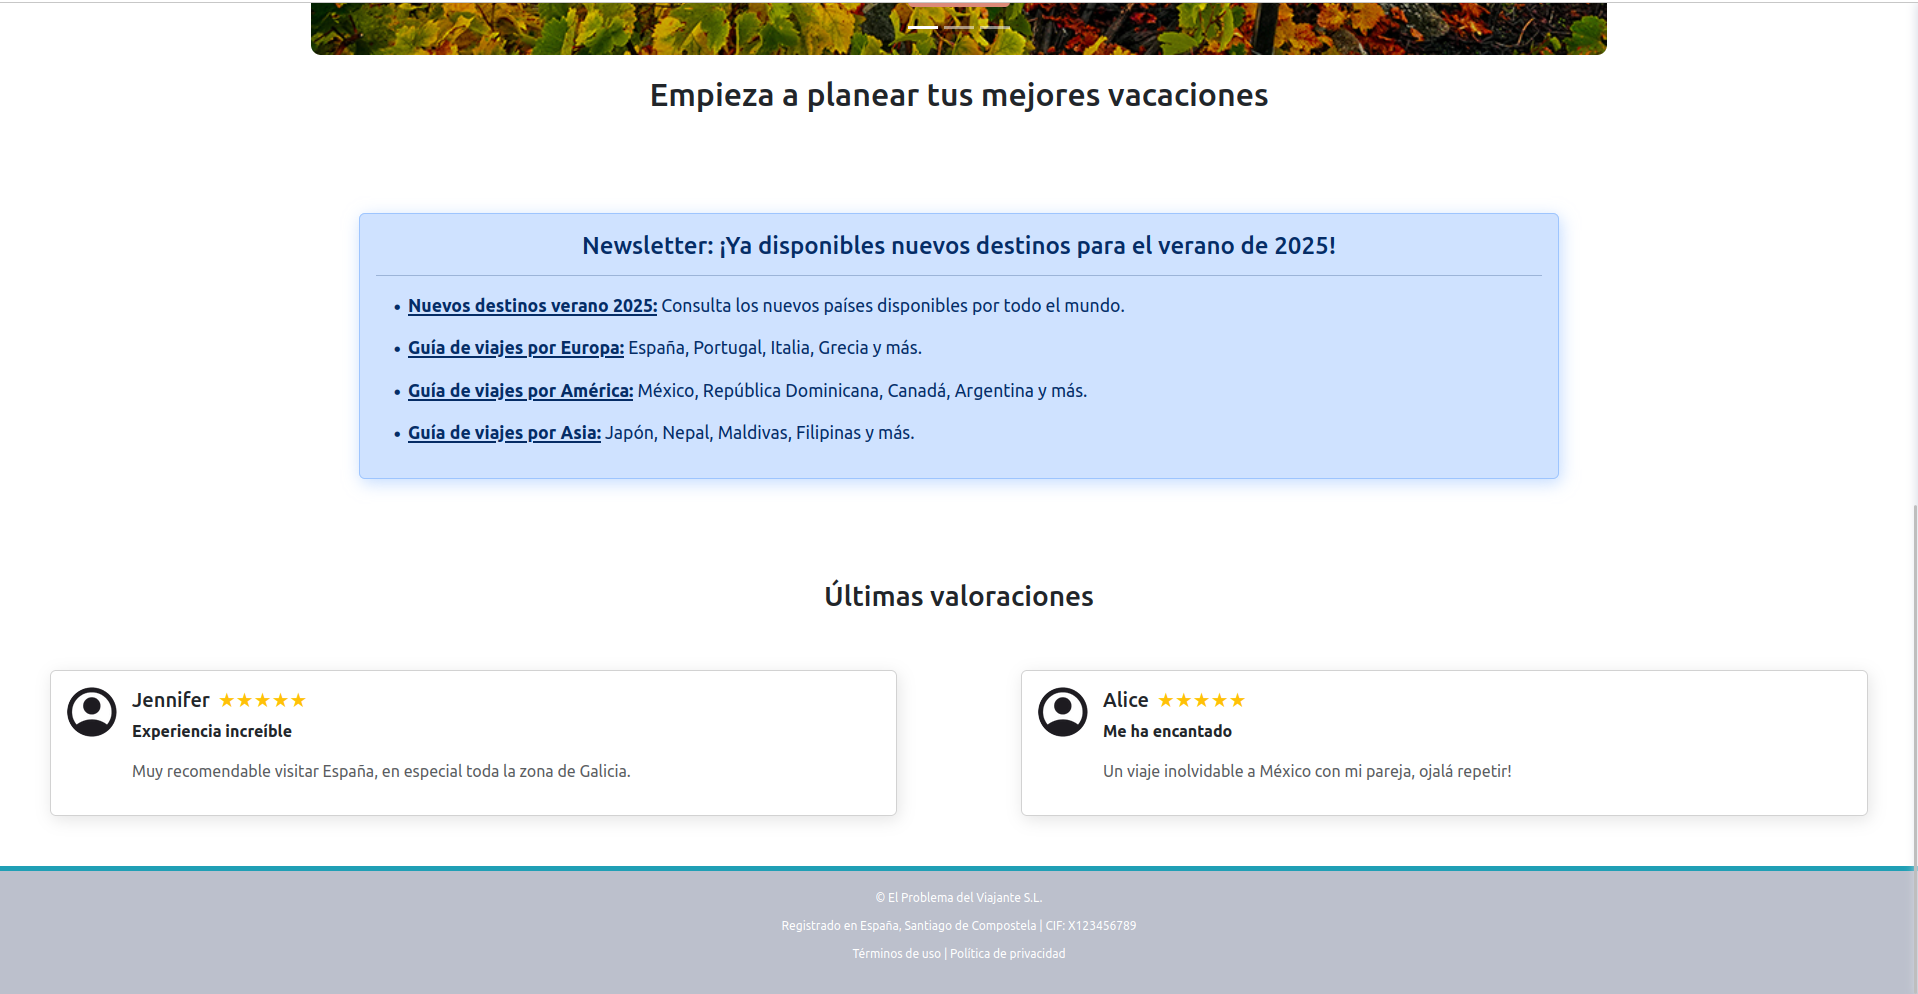
\includegraphics[width=\textwidth]{CSS/1-2 1920.png}
		\caption{Página principal - Ancho 1920px}
	\end{figure}

	Se muestra el carrusel de fotos como elemento principal, lo cual es una característica muy atractiva para el usuario, con el objetivo de que muestre interés en el contenido del resto de la página. Más abajo se encuentra un recuadro de noticias recientes y un apartado de valoraciones ficticias de otros usuarios de la página.

	\begin{figure} [H]
		\centering
		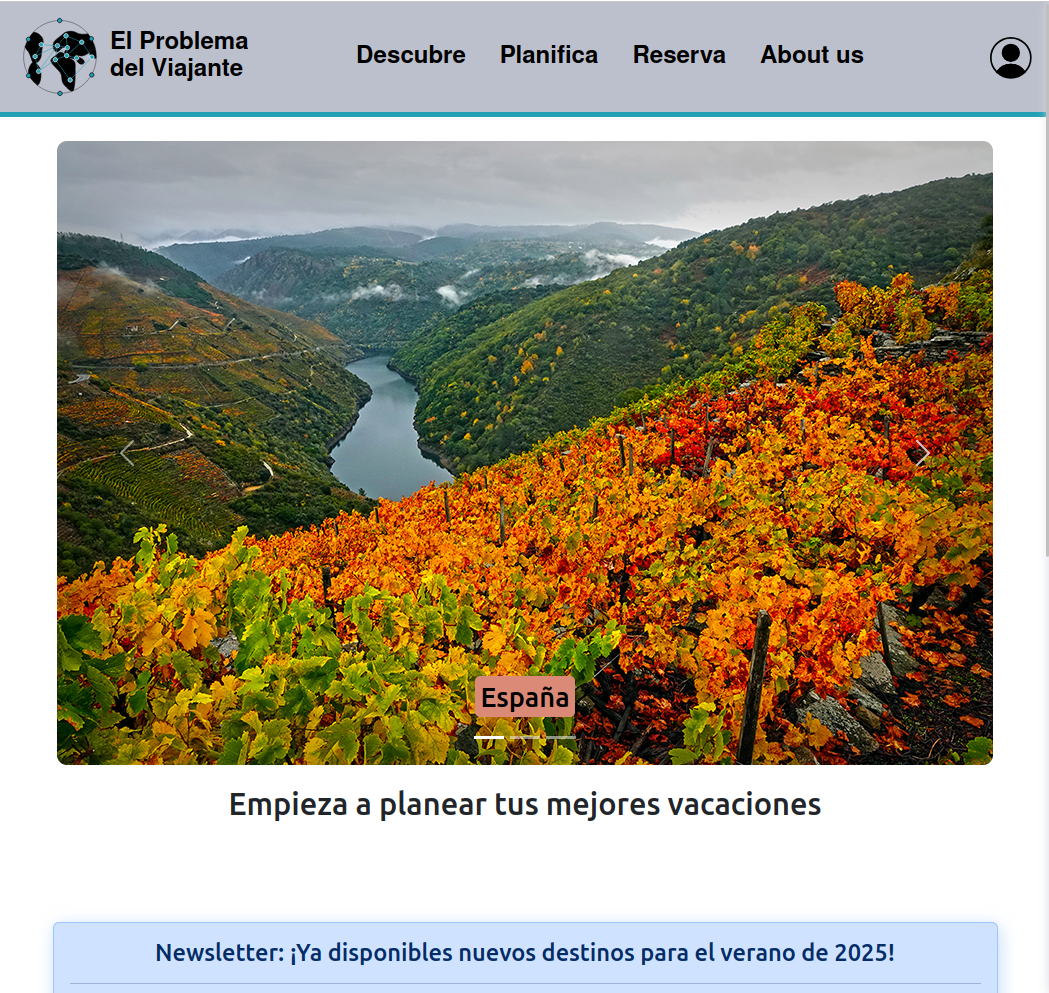
\includegraphics[height=0.4\textheight]{CSS/1-3 1024.png}
		\caption{Página principal - Ancho 1024px}
	\end{figure}
	
	Otro aspecto positivo de utilizar \textit{Bootstrap} es que él mismo gestiona los puntos de ruptura, lo cual también facilita el formateo de la página. Otro elemento destacable es que se han incluido imágenes de diferentes tamaños con el objetivo de minimizar el ancho de banda utilizado, especialmente pensado para dispositivos móviles, los cuales suelen tener conexiones más inestables.

	\begin{figure} [H]
		\centering
		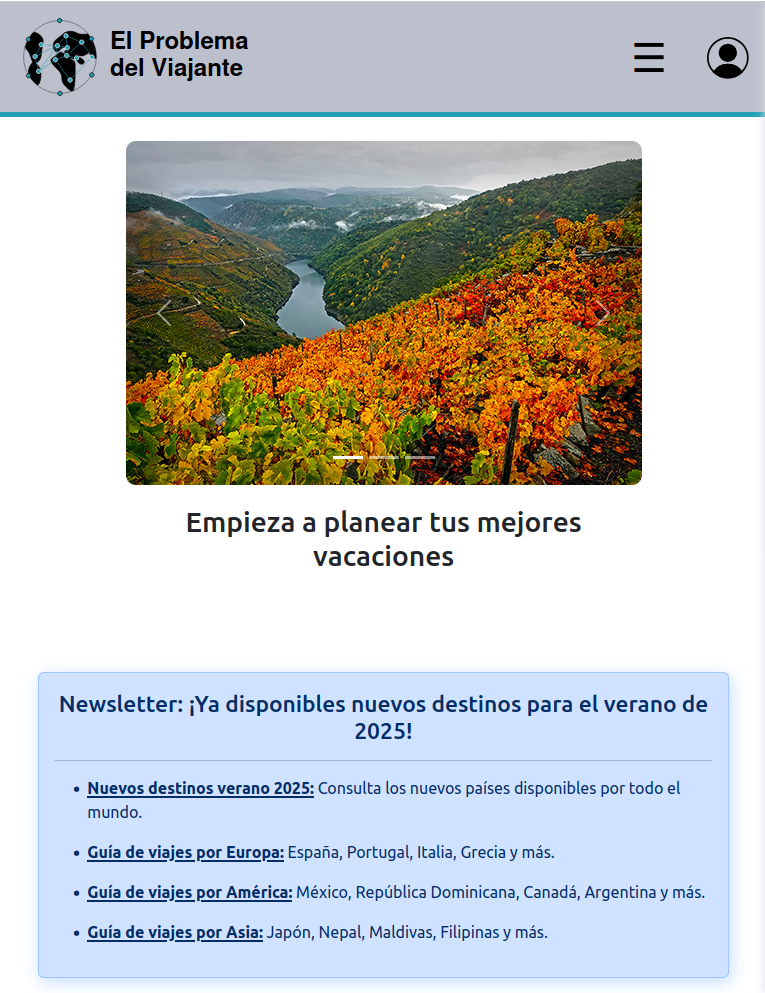
\includegraphics[height=0.4\textheight]{CSS/1-5 768.png}
		\caption{Página principal - Ancho 768px}
	\end{figure}
	\begin{figure} [H]
		\centering
		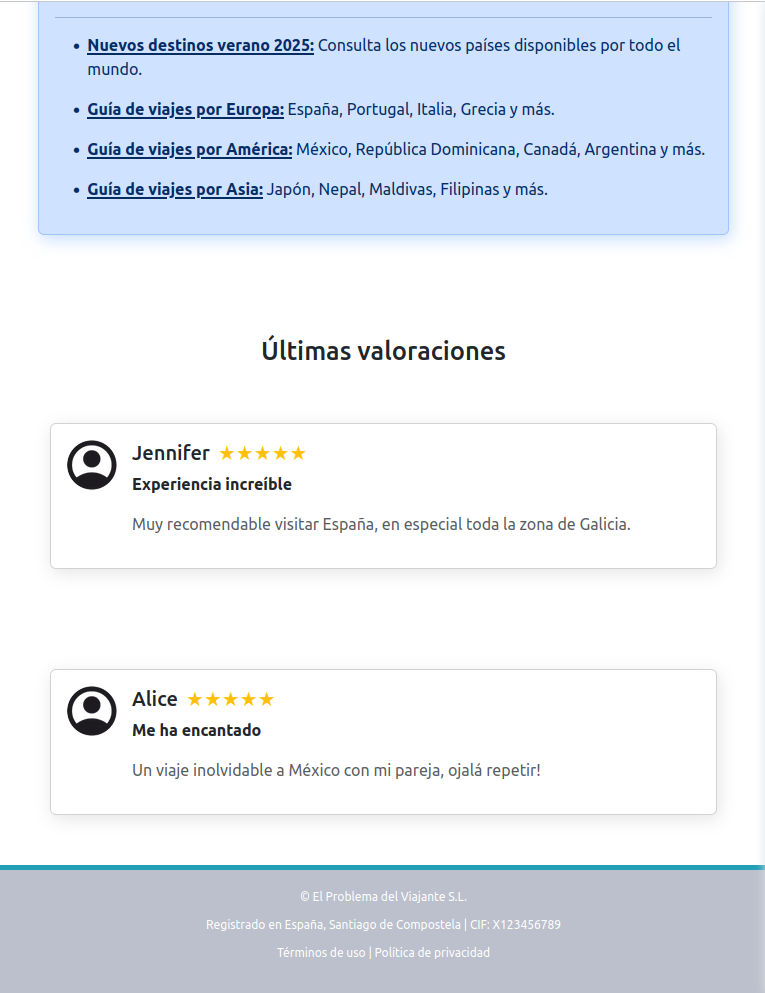
\includegraphics[height=0.4\textheight]{CSS/1-6 768.png}
		\caption{Página principal - Ancho 768px}
	\end{figure}

	Finalmente se muestra la versión de móvil, con su respectiva imagen del carrusel redimensionada y con un diseño a una columna de las valoraciones de usuarios.
	
	\begin{figure} [H]
		\centering
		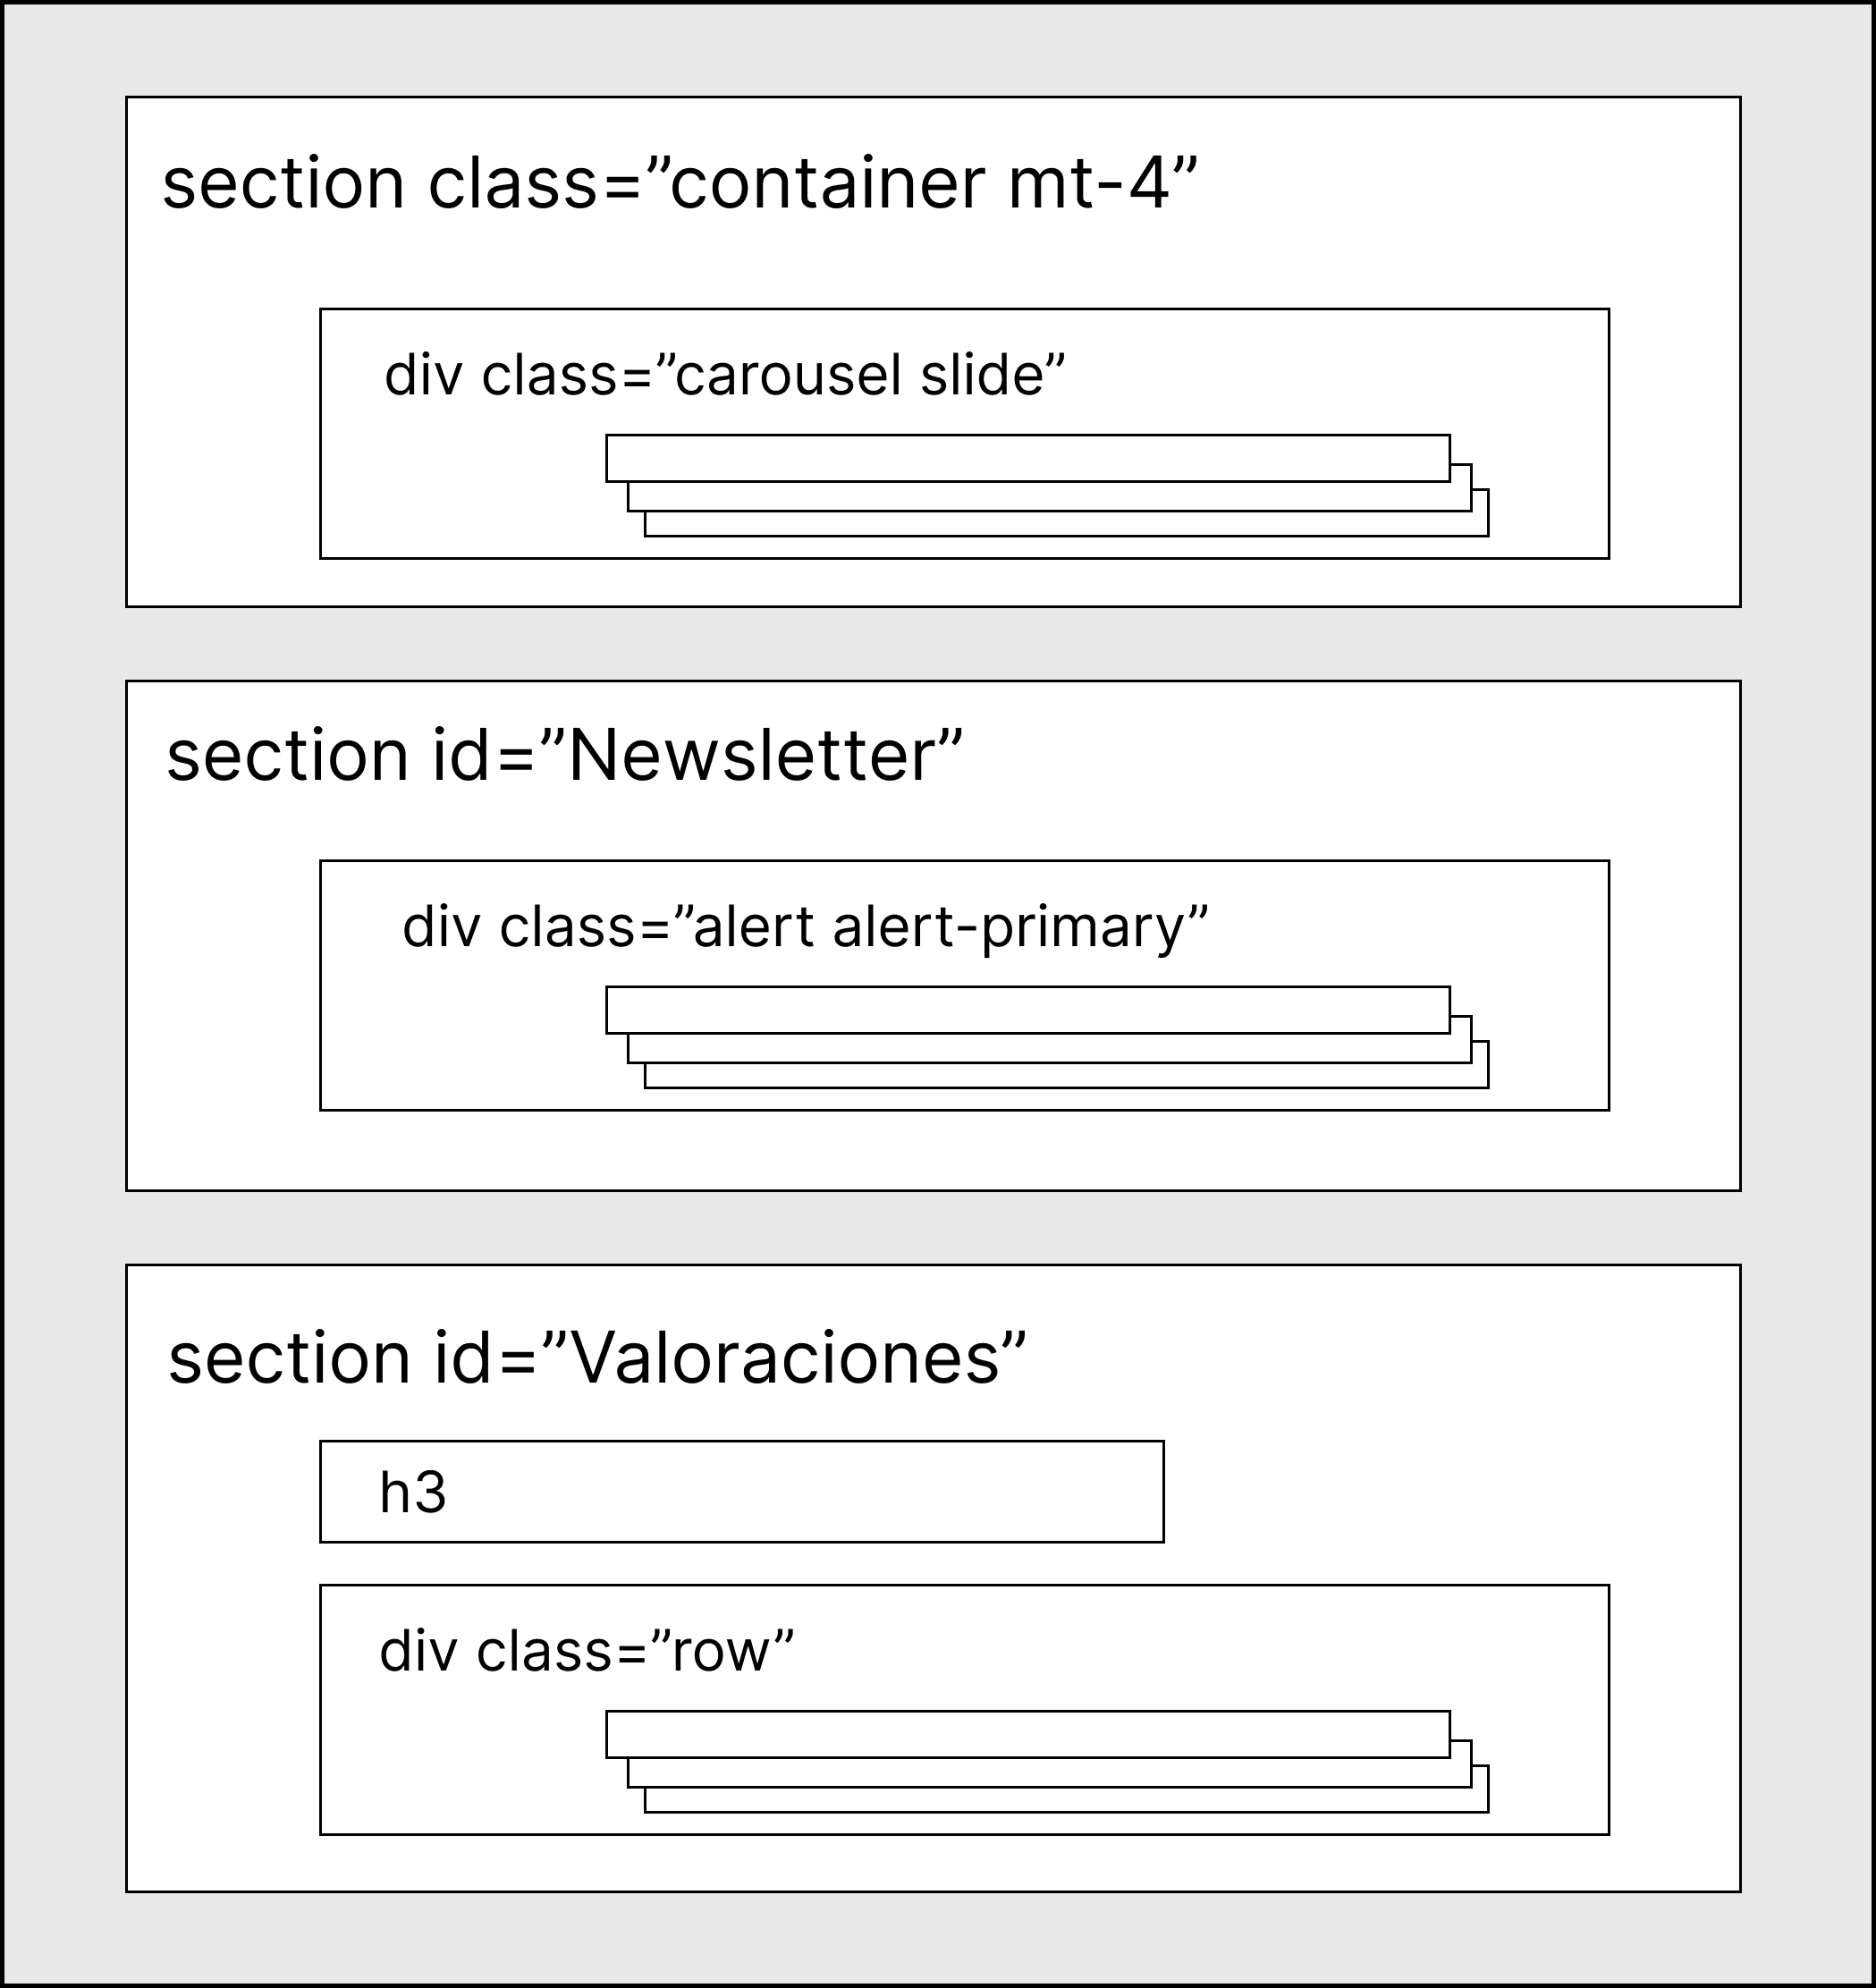
\includegraphics[width=0.7\textwidth]{CSS/CSS Principal.jpg}
		\caption{Esquema Página principal}
	\end{figure}
	
	Una de las mayores desventajas que se ha encontrado con el uso de \textit{Bootstrap} es la gran cantidad de \textbf{divs} necesarios para organizar el contenido, debido a que hay que utilizar las clases predeterminadas de la librería. Solo se incluyen en este caso los \textbf{divs} más exteriores de cada elemento relevante para facilitar la comprensión de la imagen, los cuales son el carrusel de fotos, el recuadro de noticias y la sección de valoraciones.
	
	
	
	\section{Otros elementos de CSS}
	Aunque no se mencionen explícitamente, hay otros muchos elementos de la página que son también responsivos con el objetivo de mejorar la apariencia visual y de ayudar al usuario a reconocer en qué lugar está situado el ratón. Es por eso que en muchas páginas se pueden encontrar:
	
	\begin{itemize}
		\item Elementos que al situar el ratón encima cambian de color. Por ejemplo, en el menú de navegación o en el calendario.
		\item Elementos que resaltan la caja que los contiene, como en la sección de redes sociales de About us y en las tarjetas de Reserva.
		\item Elementos que se mueven ligeramente hacia arriba al situar el ratón encima y aumentan la sombra de su caja, de forma que parezca que el elemento sobresale de la pantalla, destacándolo. 
	\end{itemize}
	
	Las páginas no principales incluyen un formateo sencillo, pues son en su mayoría bloques de texto. En ellas, solo se ajusta que aparezca el contenido en el centro de la página, y se adapte al ancho de la pantalla junto al tamaño de letra y al interlineado.
	
	
	
	
	\chapter{Documentación JavaScript}	
	
	Se ha incluido código JavaScript en tres elementos principales, los cuales se comentarán ahora en qué consiste cada uno, y luego se entrará en detalles específicos en cada uno de los apartados, pues tienen varias partes.
	
	\begin{itemize}
		\item \textbf{Inclusión dinámica del menú de navegación y del pie de página}: con el objetivo de evitar copiar y pegar constantemente estos elementos, con el riesgo de realizar de forma incorrecta, en especial si se realiza un cambio, se ha decidido añadirlo mediante un código JavaScript. Este calcula la ruta desde la que se encuentra cada página, y funciona tanto con un servidor como sin él, sin importar dónde esté ubicada la raíz.
		\item \textbf{Calendario responsivo}: se ha utilizado el calendario proporcionado por la página web \href{https://flatpickr.js.org/}{flatpickr} para añadir sobre él eventos cargados desde un fichero, los cuales también se muestran en la pestaña Planifica.
		\item \textcolor{red}{Lo tuyo}
	\end{itemize}

	
	
	\section{Acceso al DOM}
	
	Se enumeran los accesos al DOM producidos en la inclusión dinámica del menú de navegación:
	
	\begin{lstlisting}
document.addEventListener("DOMContentLoaded", function () {
	// Funcion que inserta el nav
}
	\end{lstlisting}

	En primer lugar, se crea un \textit{listener} con una función que se ejecutará una vez que el HTML haya sido totalmente cargado y procesado por el navegador. Este tipo de acceso a eventos es la primera línea de código de todos los scripts.
	
	\begin{lstlisting}
let header = document.querySelector("header");
if (!header) {
	header = document.createElement("header");
	document.body.insertBefore(header, document.body.firstChild);
}
	\end{lstlisting}

	En segundo lugar, se busca la primera etiqueta \textbf{header} de la página, donde debe ir el menú de navegación. En caso de no encontrarla, se crea llamando a la función \texttt{createElement()}, la cual permite insertar un nuevo nodo en el DOM. Y luego se accede a un elemento del DOM, en concreto al primer nodo del cuerpo del documento, que es donde debe insertarse el menú de navegación.	Por tanto, hay tres nuevos accesos al DOM en esta zona del código. 
	
	\begin{lstlisting}
const navContainer = document.createElement("nav");
navContainer.className = "main-nav";
navContainer.innerHTML = `...`;

document.querySelector("header").appendChild(navContainer);
	\end{lstlisting}
	
	A continuación, se crea el nodo correspondiente al menú de navegación, se inserta el contenido y se realiza un nuevo acceso a elementos del DOM, insertando mediante \texttt{appendChild()} un nuevo hijo al \textbf{header}, que ya se sabe que se encuentra en el código HTML por el apartado anterior.
	
	\begin{figure} [H]
		\centering
		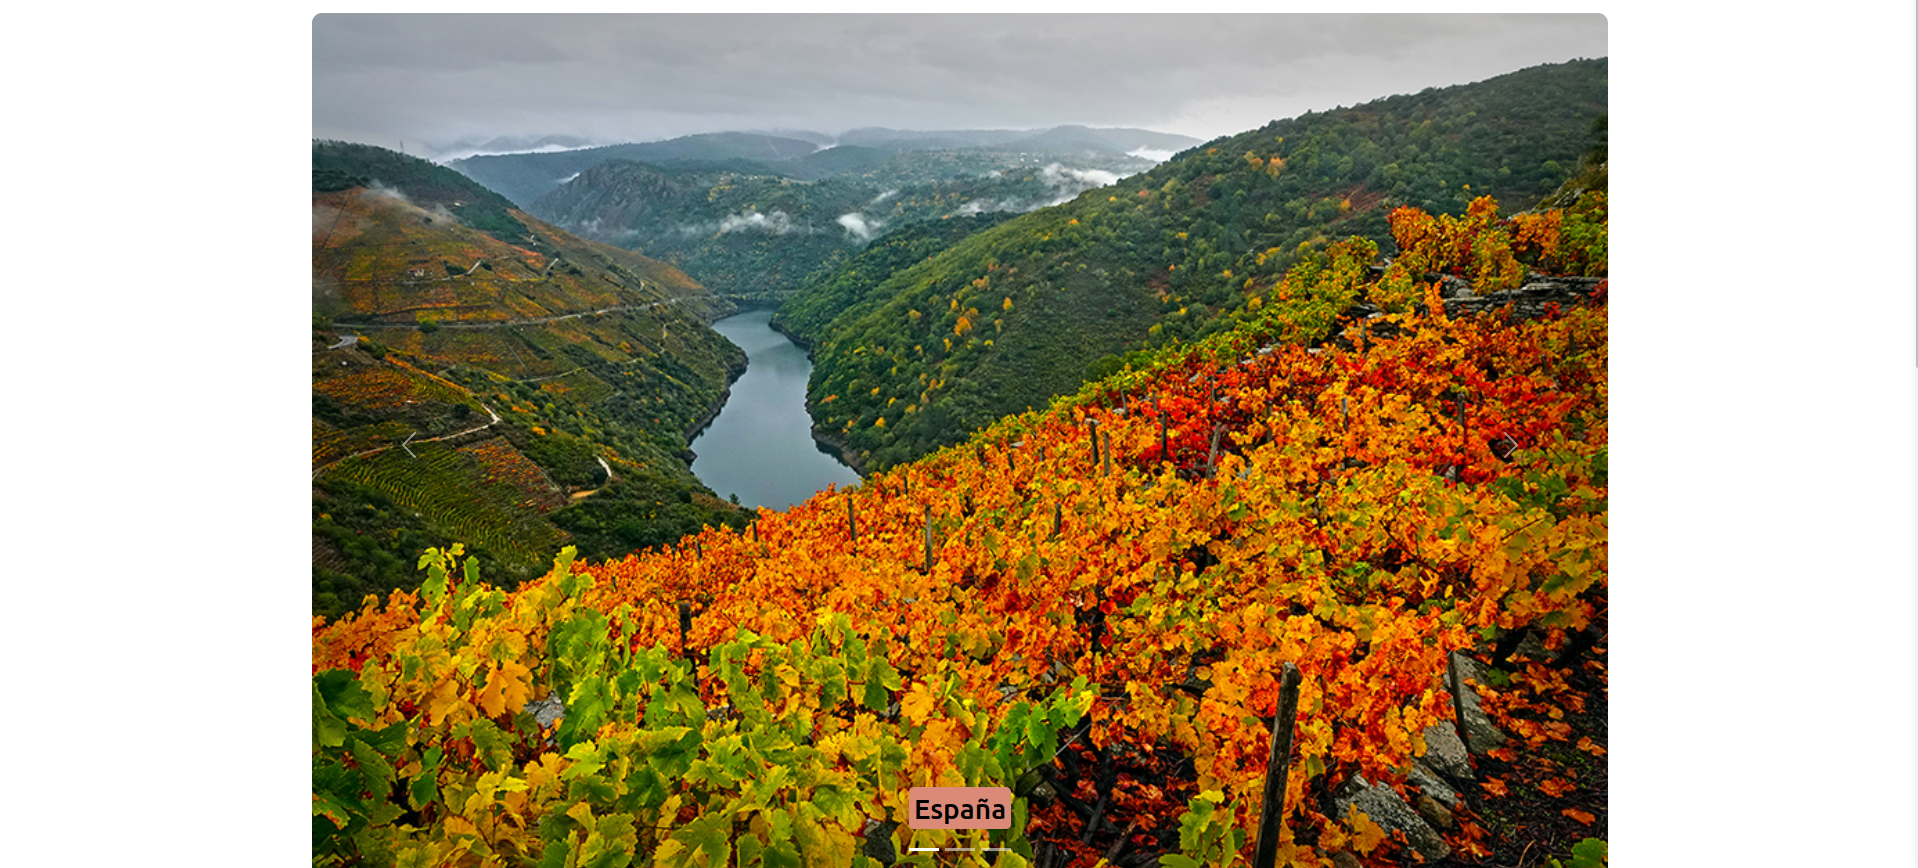
\includegraphics[width=\textwidth]{CSS/1-1 1920cut.png}
		\caption{Página principal sin el menú de navegación}
	\end{figure}
	\begin{figure} [H]
		\centering
		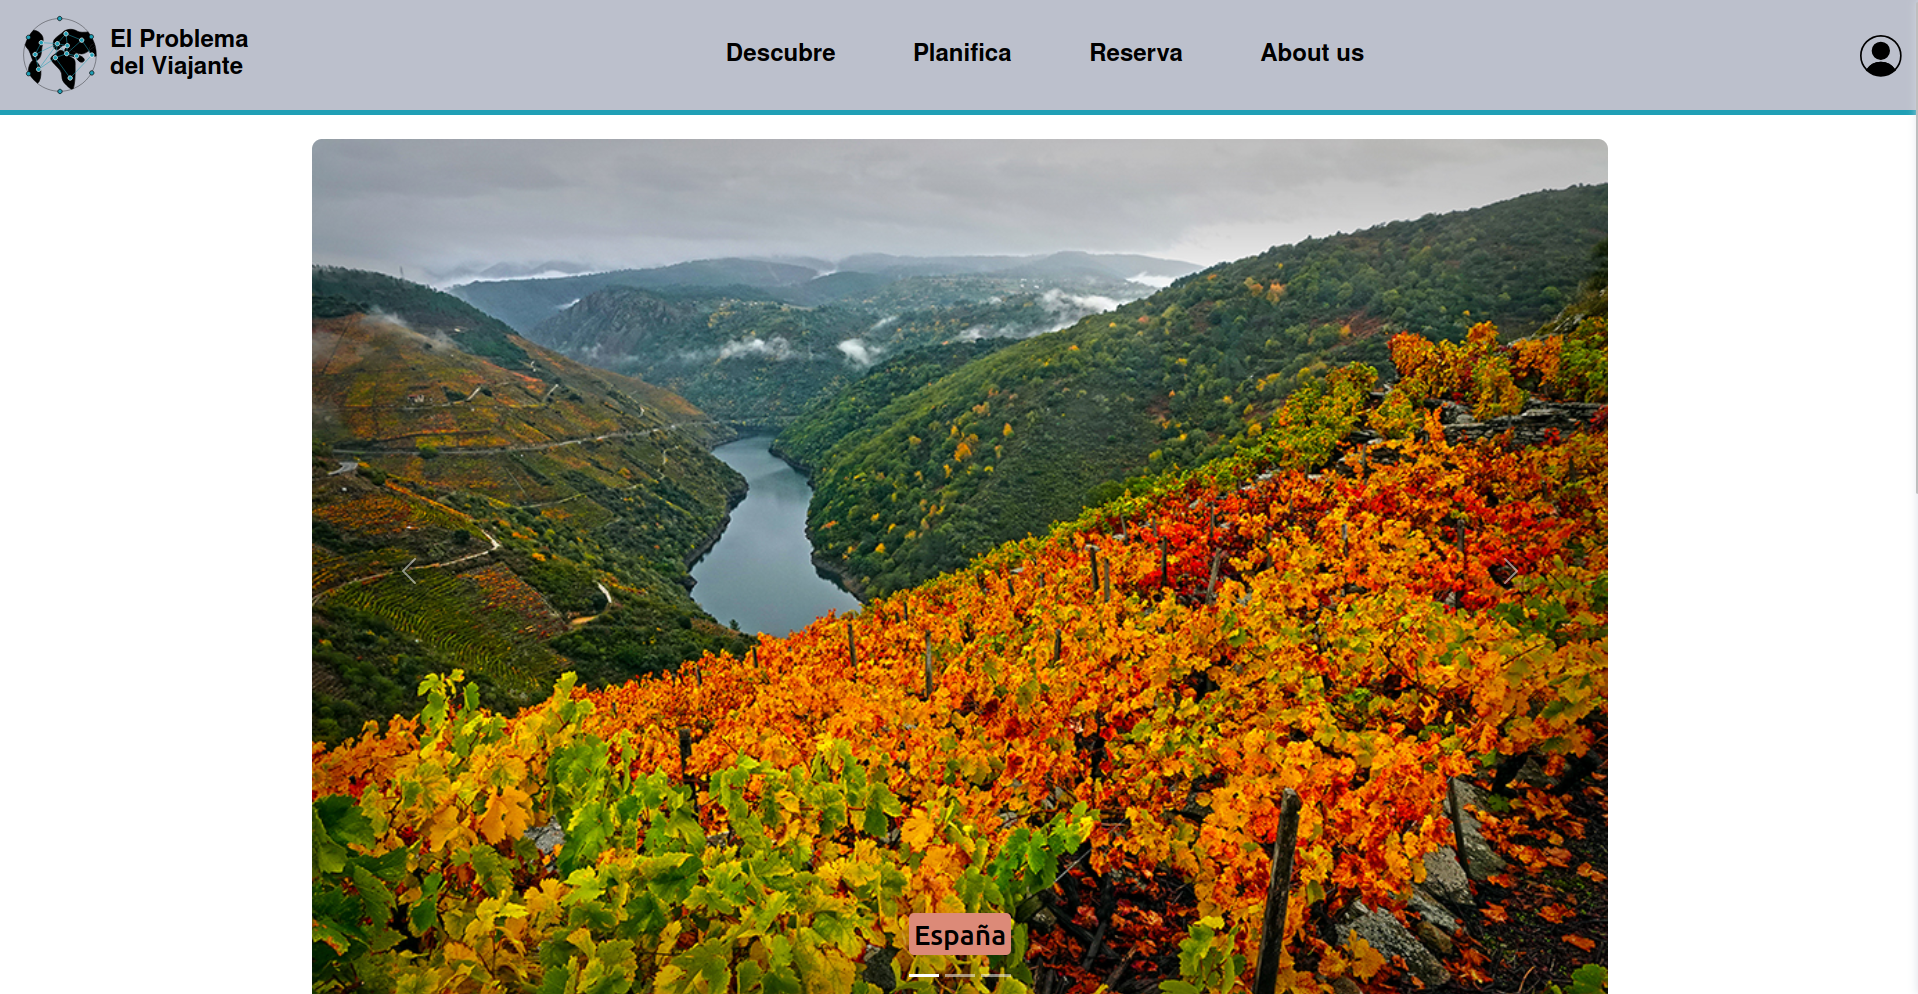
\includegraphics[width=\textwidth]{CSS/1-1 1920.png}
		\caption{Página principal con el menú de navegación}
	\end{figure}

	En este caso no hay elementos que cambien dinámicamente, por lo que solamente se pueden mostrar dos imágenes de las grandes diferencias que produce en el aspecto de la página un menú de navegación visualmente interesante respecto de no tenerlo.
	
	
	\begin{lstlisting}
const mobileMenu = document.getElementById("mobile-menu");
const closeButton = document.getElementById("close-menu");
	\end{lstlisting}

	Para finalizar, se incluyen dos accesos a elementos del DOM que devuelve el nodo cuyo id coincide con el nombre indicado. Estos se utilizan para la gestión del menú de navegación para móviles, que se crea mediante una barra lateral. Solamente en el código del menú de navegación hay muchas más accesos al DOM de todo tipo, pero aquí solo se incluyen algunos de los más relevantes para la comprensión del código.
	
	\begin{figure} [H]
		\centering
		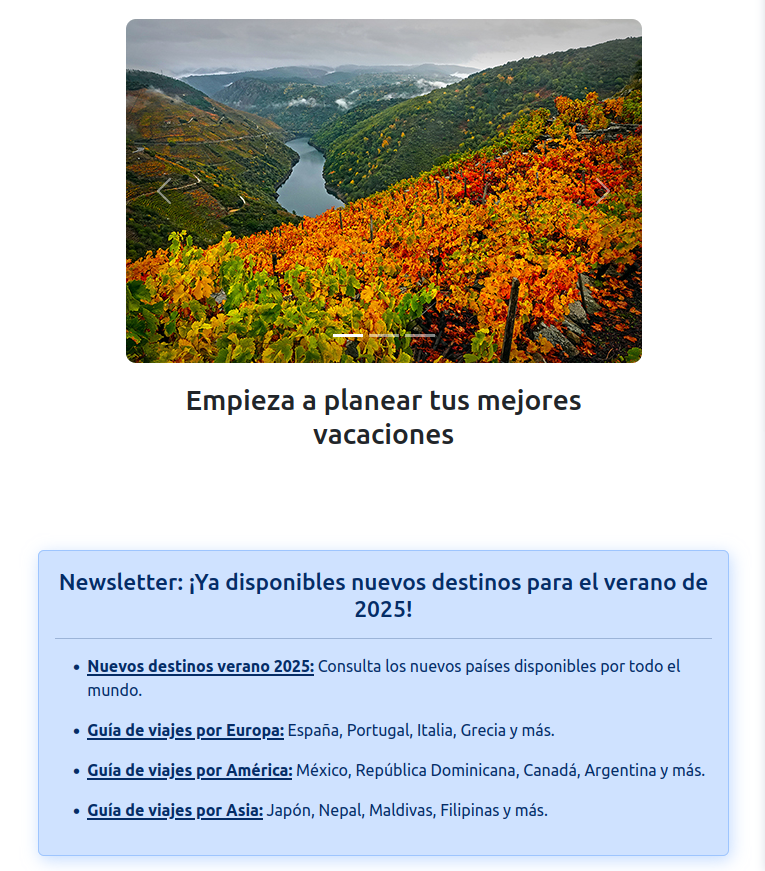
\includegraphics[height=0.4\textheight]{CSS/1-5 768cut.png}
		\caption{Página principal sin el menú de móvil}
	\end{figure}
	\begin{figure} [H]
		\centering
		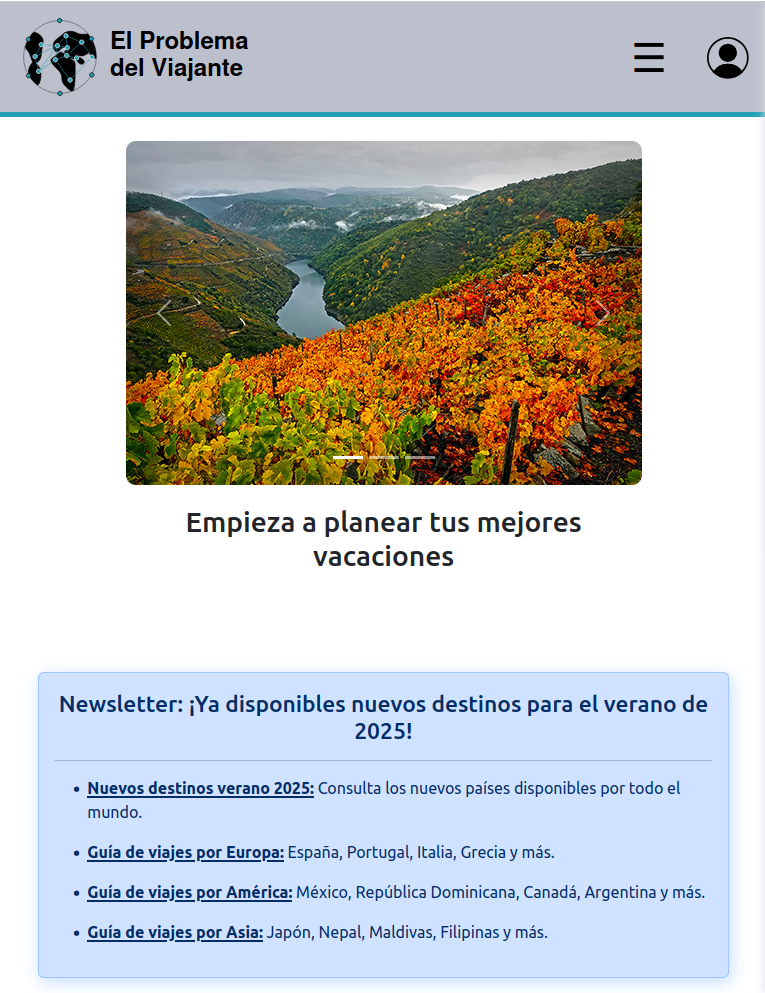
\includegraphics[height=0.4\textheight]{CSS/1-5 768.png}
		\caption{Página principal con el menú de móvil}
	\end{figure}

	\subsection{Respuesta a eventos}

	En relación con el menú de móvil, también hay que comentar la respuesta a eventos, la cual es necesaria para el funcionamiento correcto del mismo, ya que requiere desplazar la barra lateral a una zona visible de la pantalla, y que desaparezca cuando se cierra.
	
	\begin{lstlisting}
mobileMenu.addEventListener("click", function () {
	menuSidebar.classList.add("open"); // Muestra el menu
	body.classList.toggle("open"); // Ajuste del ancho
});
	\end{lstlisting} 

	En el elemento \texttt{mobileMenu} que se ha mencionado anteriormente que se obtiene mediante un acceso al DOM, se añade un \textit{listener} que ejecuta la función mostrada cuando se hace click sobre el botón del menú. Cuando se pulsa con el ratón, se muestra el menú mediante una transición realizada con CSS y ajusta la clase \texttt{open}, alternando entre el estado abierto y cerrado, lo cual permite activar y desactivar estilos dinámicamente. El botón de cierre tiene un funcionamiento similar, por lo que no se incluye.
	
	\begin{figure} [H]
		\centering
		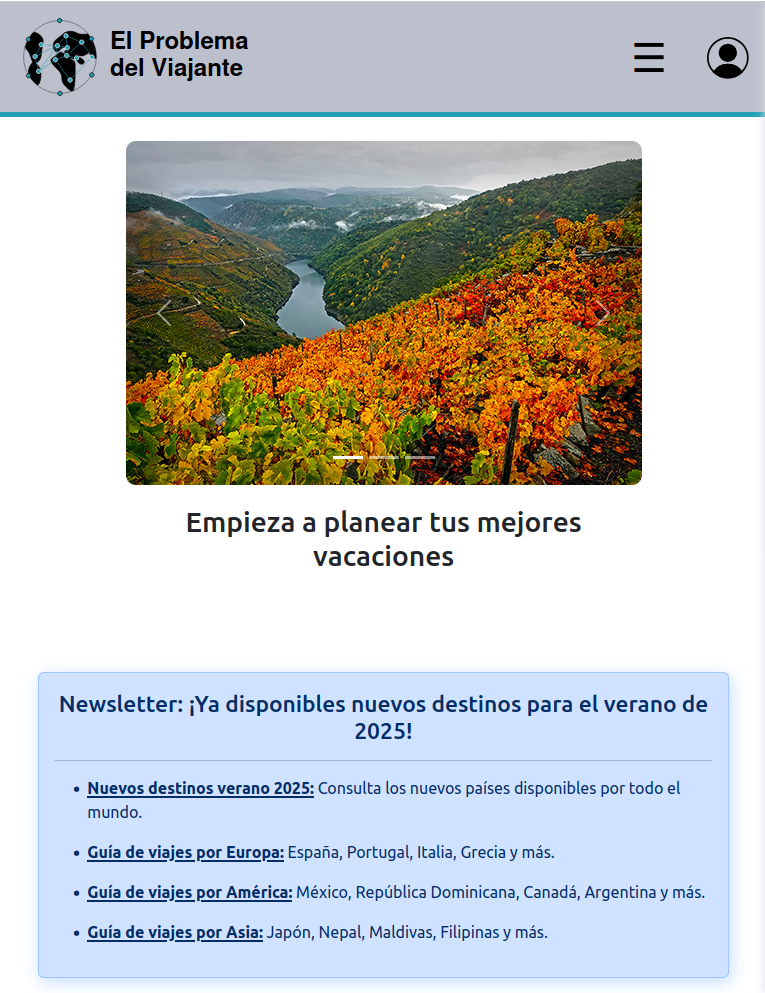
\includegraphics[height=0.4\textheight]{CSS/1-5 768.png}
		\caption{Menú de móvil cerrado}
	\end{figure}
	\begin{figure} [H]
		\centering
		\includegraphics[height=0.4\textheight]{CSS/1 extra1.png}
		\caption{Menú de móvil abierto}
	\end{figure}

	En las dos imágenes anteriores se muestra el funcionamiento del menú de móvil aunque, debido a que las fotos son estáticas, se pierde la información relativa a la responsividad de los botones y las transiciones creadas con CSS que otorgan una mejor experiencia de usuario.
	
	\begin{lstlisting}
function checkScreenSize() {
	menuLinks.style.display = window.innerWidth > 900 ? "flex" : "none";
	if (window.innerWidth > 900) menuSidebar.classList.remove("open");
}

window.addEventListener("resize", checkScreenSize);
	\end{lstlisting}

	Otro evento incluido en este script está relacionado con los cambios en el tamaño de la pantalla. Cuando se redimensiona la pantalla, se comprueba el ancho de esta, lo cual permite saber cuándo mostrar el menú de móvil. Además, en caso de que esté abierta la barra lateral (\texttt{menuLinks}) cuando se amplíe la pantalla a un ancho superior a 900px, esta se cierra automáticamente, con una transición suave creada con CSS.
	
	Este efecto no se puede mostrar con nuevas imágenes ya que es totalmente dinámico, y ya se han mostrado en múltiples ocasiones fotos con el menú de navegación de ordenador y de móvil.
	
	\begin{Huge}
		\textcolor{red}{Falta un evento (algo con un listener). Que no sea click ni resize si puede ser}
	\end{Huge}
	
	\section{Uso de jQuery y JES6}
	\begin{Huge}
		\textcolor{red}{Falta un código con jQuery}
	\end{Huge}

	En relación con JES6, se utiliza constatemente en los códigos ya mostrados, por ejemplo en el uso de \texttt{let} y \texttt{const} en la declaración de variables, o la utilización de funciones arrow.
	\begin{Huge}
		\textcolor{red}{Yo mucho JES6 no tengo. Si tienes algo mejor mételo}
	\end{Huge}
	
	\section{Carga de contenido}
	En esta sección se mostrarán dos posibles formas de cargar contenido, una utilizando API Fetch para leer un archivo JSON, en el que se encuentran los eventos que luego se muestran en el calendario, y otra que \textcolor{red}{??????????????????????} para cargar un archivo XML y \textcolor{red}{habla algo del Single Page Application si quieres}
	\subsection{Formato XML}
	\begin{Huge}
		\textcolor{red}{Falta -----------------------------------}
	\end{Huge}

	\subsection{Formato JSON}
	Como se ha mencionado, se carga un archivo JSON sencillo que incluye los próximos eventos relevantes para el usuario, los cuales se muestran en el calendario. El formato utilizado en el archivo JSON es
	
	\begin{lstlisting}
{"events": [
	{ "date": "fecha1", "title": "Evento1" },
	{ "date": "fecha2", "title": "Evento2" },
    { ... }
]}
	\end{lstlisting}

	Este archivo se carga en el script del calendario de la siguiente forma.
	
	\begin{lstlisting}
async function loadEvents() {
	try {
		const response = await fetch(rootPath + "/data/events.json", { cache: "no-cache" });
		const data = await response.json();
		/* ... Gestion de errores, no se incluye ... */
		return data.events;
	} catch (error) {
		console.error("Error cargando eventos:", error);
		return [];
	}
}

loadEvents().then(function (events) {
	initCalendar(events);
});
	\end{lstlisting}
	
	Este código lleva al cliente el archivo indicando en la función \texttt{fetch()}, y lo lee, devolviendo un array con los eventos en caso de éxito, es decir, que el archivo ha sido procesado correctamente. En ese caso, se ejecuta la función \texttt{initCalendar()}, la cual no se incluye ya que principalmente se encarga de configurar el calendario para mostrar de la forma adecuada (en español, que el primer día de la semana sea el lunes, etc.). Sí que es interesante comentar una de las funciones a las que llama \texttt{initCalendar()}, que se muestra a continuación.
	
	\begin{lstlisting}
function highlightEvents(instance, events) {
	setTimeout(function () {
		let days = instance.calendarContainer.querySelectorAll(".flatpickr-day");
		
		days.forEach(function (day) {
			let date = formatLocalDate(day.dateObj); // Formato YYYY-MM-DD
			// Comprobar si la fecha está en la lista de eventos
			if (markedDates.includes(date)) {
				day.classList.add("event-day");
			}
		});
	}, 100);
	
}
	\end{lstlisting}
	
	Esta función se encarga de resaltar los días en los que hay algún evento. Para ello, se accede al DOM para obtener todos los nodos que son un día, y para cada uno se comprueba si existe algún evento cuya fecha coincida con la del propio días. En caso afirmativo, se añade la clase \texttt{event-day}, la cual muestra el día de color rojo. Los días marcados también se añaden en una lista al lado del calendario junto con su título, aunque este código no se muestra debido a su simplicidad.
	
	\begin{figure} [H]
		\centering
		\includegraphics[height=0.4\textheight]{CSS/3 extra1.png}
		\caption{Calendario sin eventos}
	\end{figure}

	\begin{figure} [H]
		\centering
		\includegraphics[height=0.4\textheight]{CSS/3 extra2.png}
		\caption{Calendario con eventos}
	\end{figure}
	

	En las dos imágenes anteriores se muestran las grandes diferencias entre el calendario por defecto de flatpickr y las modificaciones añadidas con JavaScript. De nuevo, hay detalles que no se muestran en las imágenes como la responsividad al pasar el ratón por encima de los días del calendario, o por encima de la lista de eventos.
	
	
	
	\chapter{Anexo}
	\label{chap:anexo1}
	\section{Tormenta de ideas}
	
	Todos los elementos obtenidos durante la tormenta de ideas son:
	
	\begin{itemize}
		\item Presentación de la página
		\item Destinos de moda/recomendados
		\item Exploración (lugares menos conocidos, o aleatorios)
		\item About us: quiénes somos, nuestra historia, qué nos diferencia
		\item Búsqueda de hoteles
		\item Búsqueda de medios de transporte (avión, tren, autobús, etc.)
		\item Lugares de visita, ocio, restauración, etc.
		\item Alquiler de coches
		\item Experiencias exclusivas
		\item Calendario para la planificación del viaje
		\item Mapa de lugares favoritos
		\item Newsletter con novedades
		\item FAQ
		\item Mecanismos de reserva con seguridad
		\item Seguro de viajes
		\item Consejos generales para viajes al extranjero
		\item Nuestro sistema de puntuación
		\item Opiniones de expertos
		\item Certificados de calidad, premios
		\item Redes sociales
		\item Términos de uso, política de cookies, política de privacidad
	\end{itemize}


	\section{Cambios}
	\label{sect:anexo2}
	En esta sección se incluye una lista de cambios realizados a lo largo del proyecto, que difieren respecto al diseño original que se planteó. Cada uno incluye una breve descripción y una justificación de por qué se ha hecho.
	
	\subsection{Diseño final}
	\textcolor{red}{------------------------ Hay que escribir esto bien y razonar -----------------------}
	Principal: se ha cambiado la zona principal por un carrusel con bootstrap
	About us: se han cambiado los recuadros de colores por solo los bordes de colores, para no saturar demasiado
	Planifica: lo mismo
	
	
	\subsection{Estructura de ficheros}
	La estructura de ficheros general se ha mantenido a lo largo del proyecto, aunque se ha añadido algún subdirectorio a los que se mencionan en \ref{ficheros}. Concretamente, cada una de las cinco páginas principales tiene su propio directorio dentro de /html y /images, con el objetivo de facilitar la gestión de grandes cantidades de contenido.
	
	\begin{huge}
		\textcolor{red}{Se podría incluir un tree para enseñar los archivos, o lo que se ve en el IDE}
	\end{huge}
	
	
	
	\begin{thebibliography}{widestlabel}
		\href{https://html.spec.whatwg.org/multipage/}{W3C}
		Aquí deberían ir páginas de consulta (w3schools, bootstrap, flatpickr, etc.), y quizás páginas en las que nos hemos inspirado
	\end{thebibliography}
	
	
	
\end{document}